%yright 2007, 2008, 2009 Elsevier Ltd
%% 
%% This file is part of the 'Elsarticle Bundle'.
%% ---------------------------------------------
%% 
%% It may be distributed under the conditions of the LaTeX Project Public
%% License, either version 1.2 of this license or (at your option) any
%% later version.  The latest version of this license is in
%%    http://www.latex-project.org/lppl.txt
%% and version 1.2 or later is part of all distributions of LaTeX
%% version 1999/12/01 or later.
%% 
%% The list of all files belonging to the 'Elsarticle Bundle' is
%% given in the file `manifest.txt'.
%% 

%% Template article for Elsevier's document class `elsarticle'
%% with numbered style bibliographic references
%% SP 2008/03/01

% \documentclass[preprint,11pt]{elsarticle}
\documentclass[final,1p,11pt]{elsarticle}

%\documentclass[final,1p,times]{elsarticle}


%% Use the option review to obtain double line spacing
%%\documentclass[authoryear,preprint,review,12pt]{elsarticle}

%% Use the options 1p,twocolumn; 3p; 3p,twocolumn; 5p; or 5p,twocolumn
%% for a journal layout:
%% \documentclass[final,1p,times]{elsarticle}
%% \documentclass[final,1p,times,twocolumn]{elsarticle}
%% \documentclass[final,3p,times]{elsarticle}
%% \documentclass[final,3p,times,twocolumn]{elsarticle}
%% \documentclass[final,5p,times]{elsarticle}
%% \documentclass[final,5p,times,twocolumn]{elsarticle}

%%% For including figures, graphicx.sty has been loaded in
%% elsarticle.cls. If you prefer to use the old commands
%% please give \usepackage{epsfig}


\usepackage{epsfig}
%\usepackage{cite}
%\usepackage{mcite}
\usepackage{array,tabularx,epsfig,mathrsfs,graphicx,rotating}
\usepackage{ifthen}
\usepackage{amsfonts}
\usepackage{ragged2e}
\PassOptionsToPackage{hyphens}{url}
\usepackage[hyphens]{url}
\usepackage{hyperref}
\usepackage{listings}
\usepackage{subfigure}
\usepackage{epstopdf}
% Custom colors
\usepackage{color}
\usepackage{float}

% to cross text
\usepackage[normalem]{ulem} % either use this (simple) or
\usepackage{soul} % use this (many fancier options)


\hypersetup{
  colorlinks=true,
  linkcolor=blue,
  citecolor=blue,
  urlcolor=blue
}




\graphicspath{{figs/}}


\pdfinfo{
   /Author (Chekanov/Demarteau)
   /Title  (Conceptual Design Studies for a CEPC Detector)
   /CreationDate (D:20160102195600)
   /Subject (PDFLaTeX)
   /Keywords (PDF;LaTeX)
}


\textheight=22cm
\textwidth=14.5cm

\newcommand{\beq}{\begin{equation}}
\newcommand{\eeq}{\end{equation}}
\newcommand{\la}{\langle}
\newcommand{\promc}{{\sc ProMC}}
\newcommand{\ra}{\rangle}
\newcommand{\eps}{\epsilon}
\newcommand{\ud}{\mathrm{d}}
\newcommand{\Ec}{\mathcal{E}}
\newcommand{\Fc}{\mathcal{F}}
\newcommand{\Za}{\mathrm{Z_1}}
\newcommand{\Zb}{\mathrm{Z_2}}
\newcommand{\Zn}{\mathrm{Z_n}}
\newcommand{\F}{\mathrm{F}}

\chardef\til=126
\newcommand{\mev}{{\,\mathrm{MeV}}}
\newcommand{\gev}{{\,\mathrm{GeV}}}
\newcommand{\tev}{{\,\mathrm{TeV}}}
\newcommand{\GEANTfour} {\textsc{geant4}}
\journal{XXX-XXX}



\begin{document}
%50bins
\begin{figure}
\begin{center}
   \subfigure[5TeV at 20$\times$20(cm$\times$cm) in cluster] {
   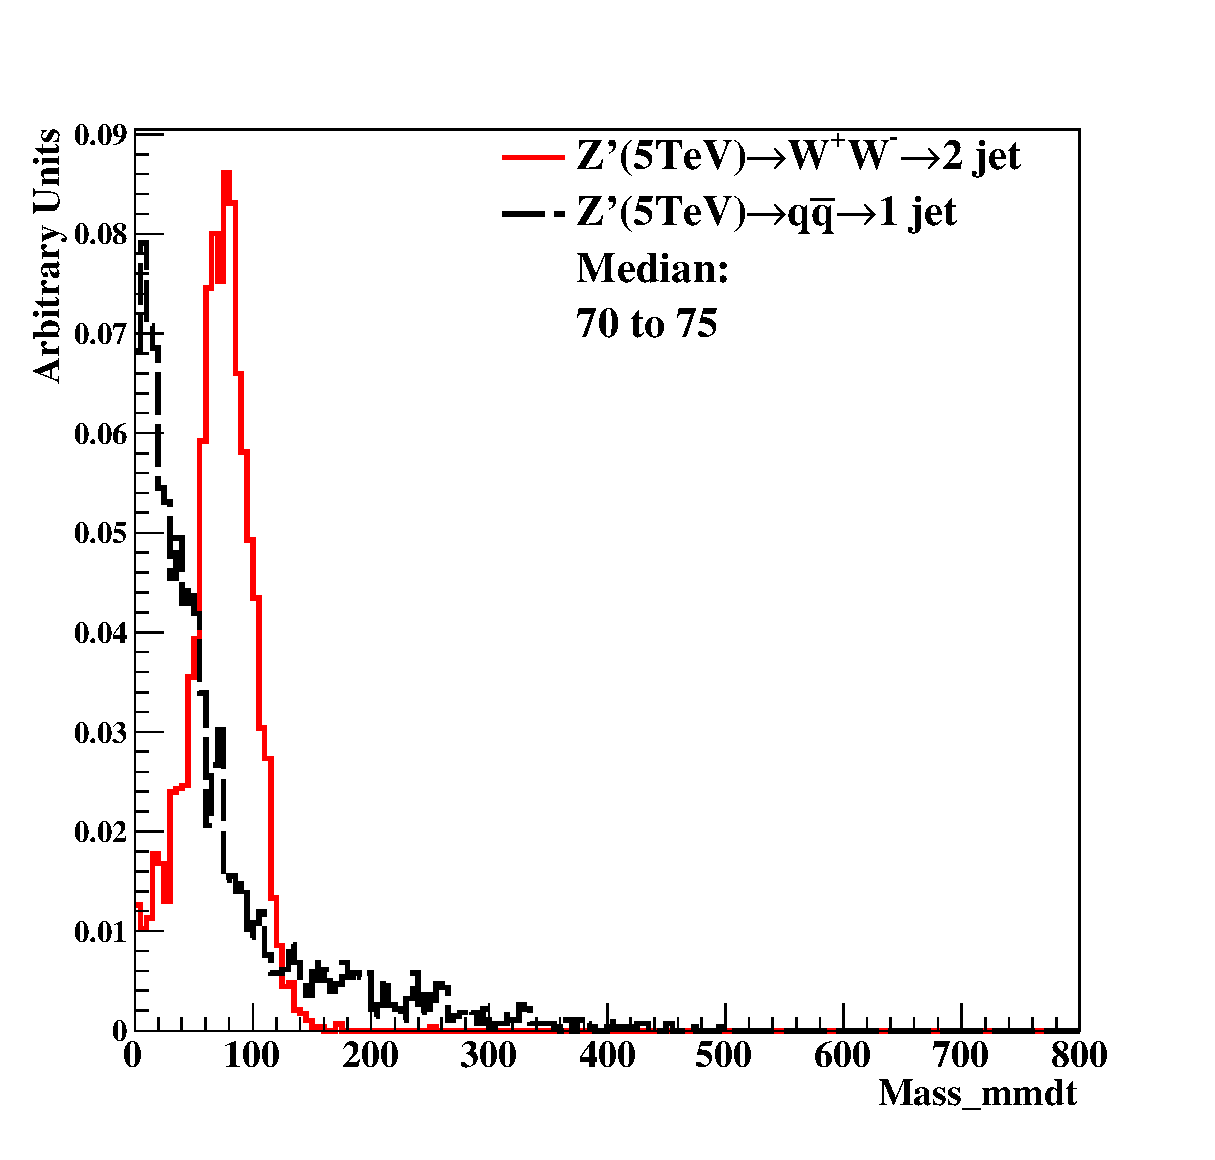
\includegraphics[width=0.43\textwidth]{figs/Dis_cluster_010_mass_mmdt_5tev_04.eps}
   }
      \subfigure[10TeV at 20$\times$20(cm$\times$cm) in cluster] {
   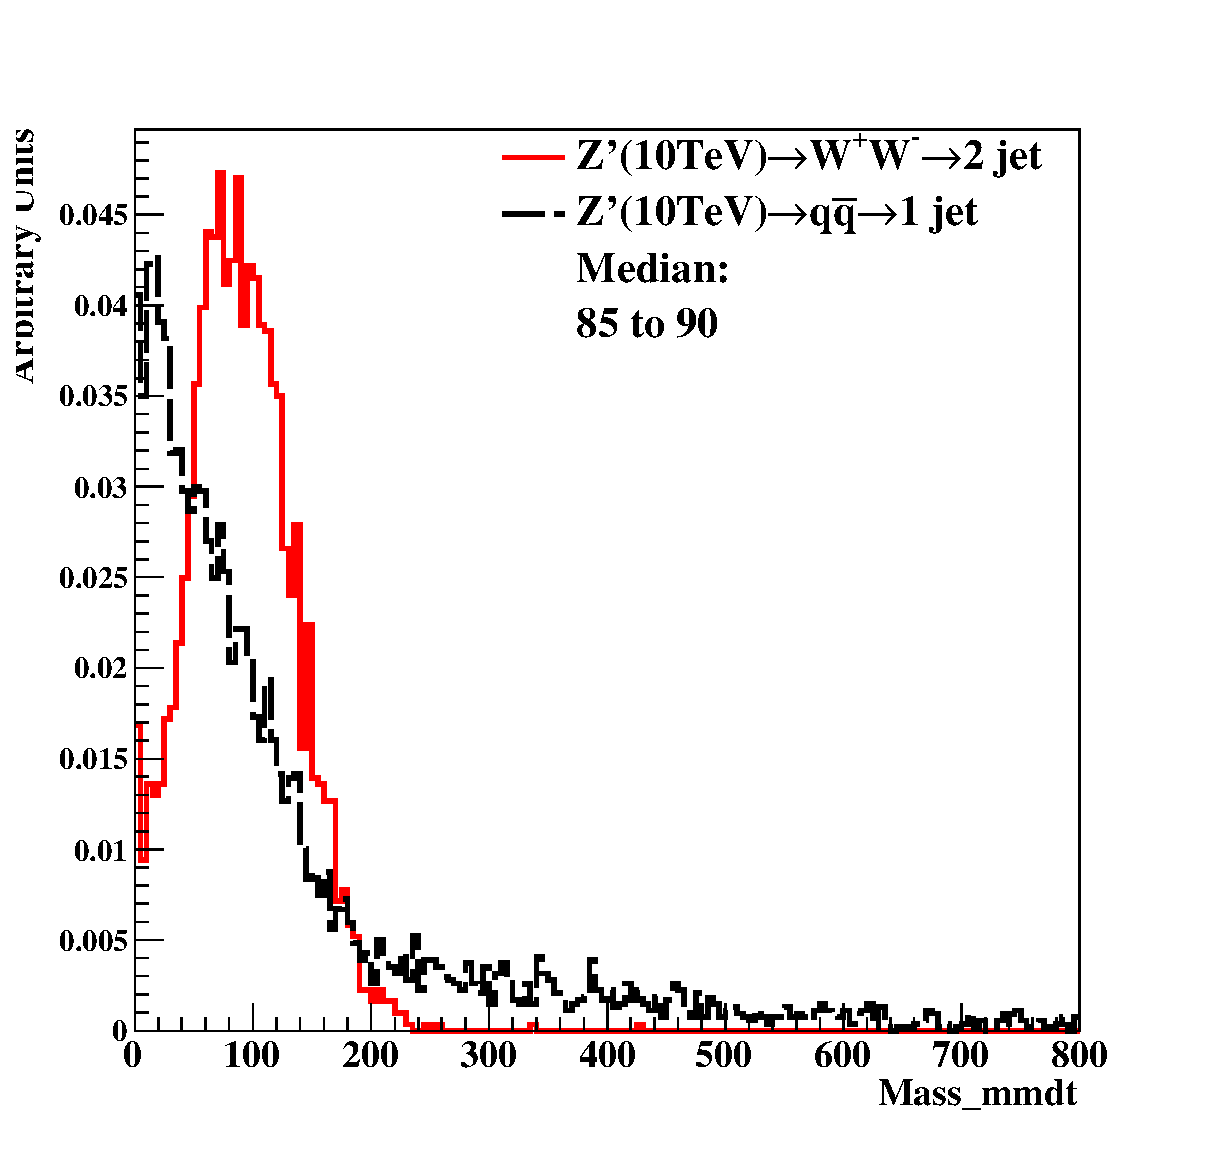
\includegraphics[width=0.43\textwidth]{figs/Dis_cluster_010_mass_mmdt_10tev_04.eps}
   }
   \subfigure[5TeV at 5$\times$5(cm$\times$cm) in cluster] {
   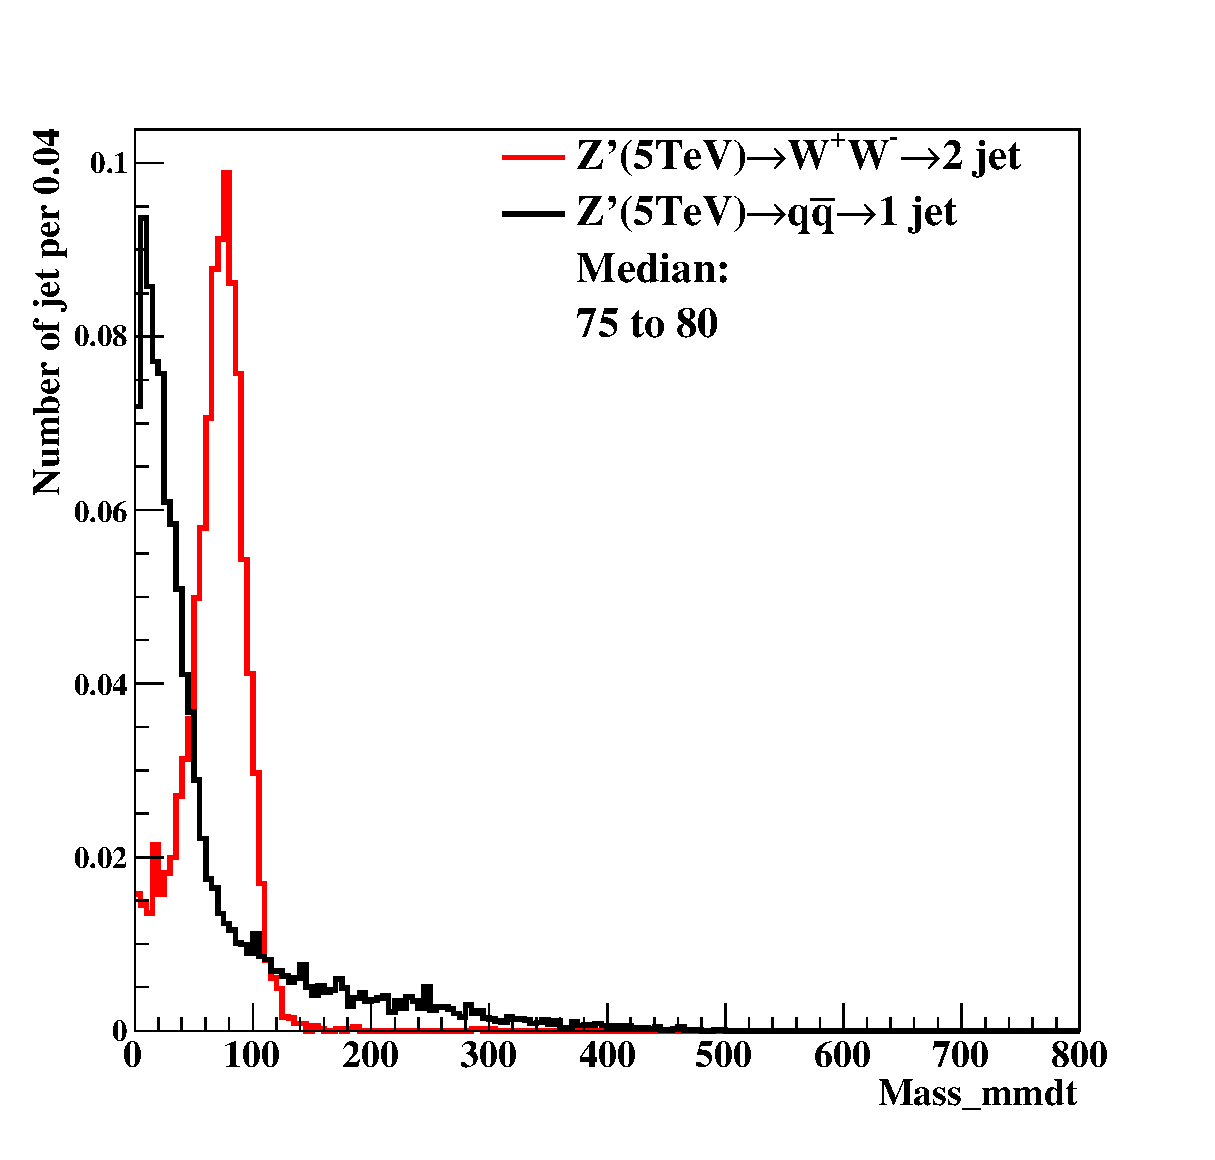
\includegraphics[width=0.43\textwidth]{figs/Dis_cluster_009_mass_mmdt_5tev_04.eps}
   }
    \subfigure[10TeV at 5$\times$5(cm$\times$cm) in cluster] {
   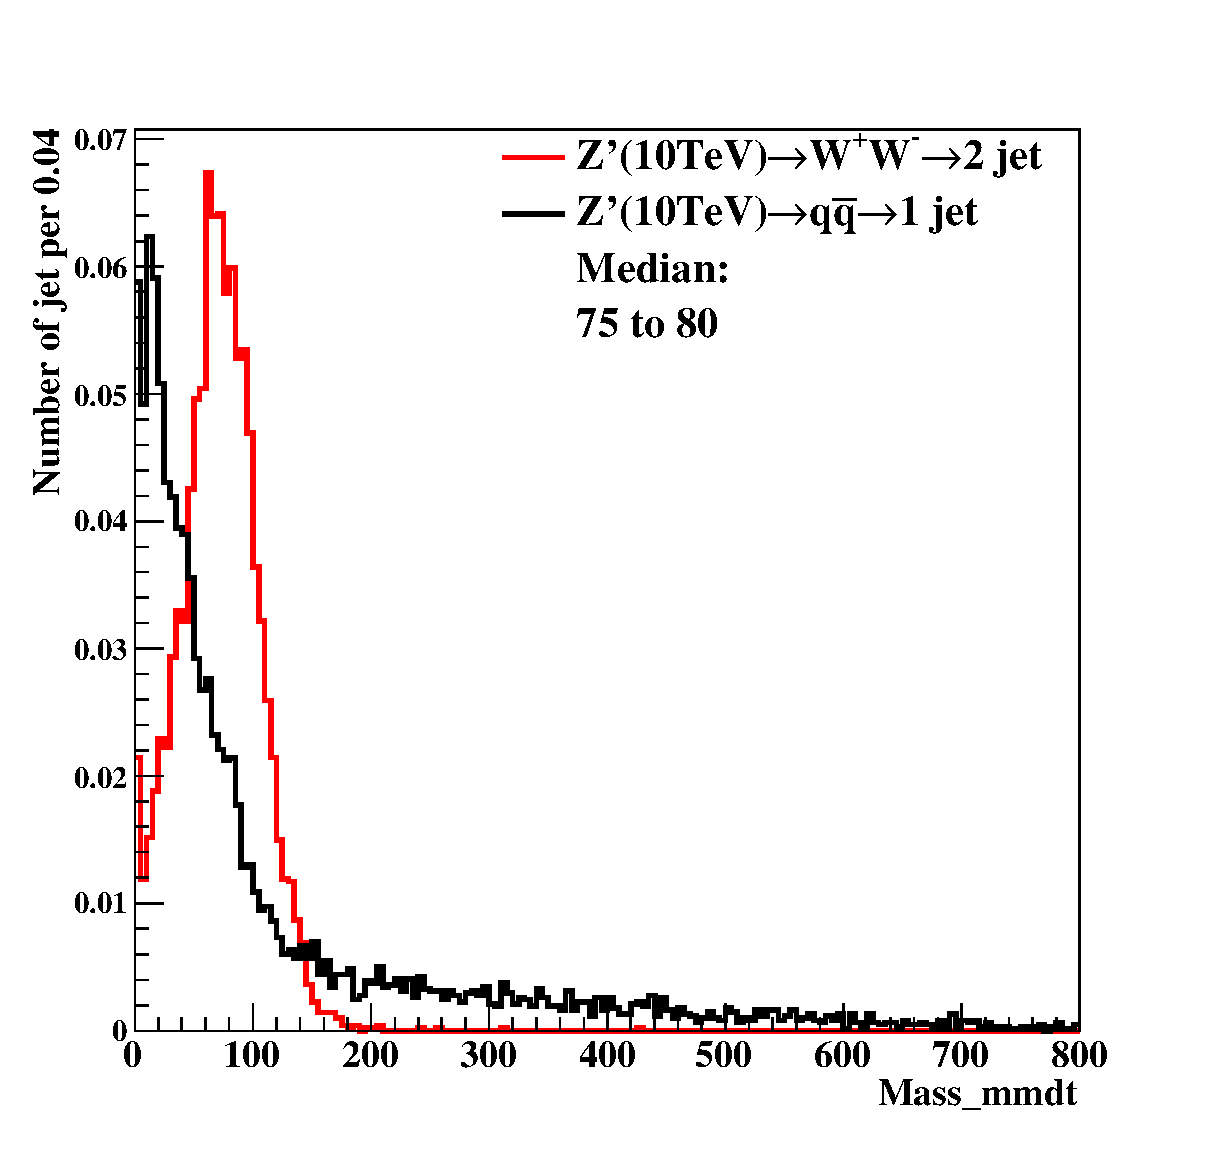
\includegraphics[width=0.43\textwidth]{figs/Dis_cluster_009_mass_mmdt_10tev_04.eps}
   }
   \subfigure[5TeV at 1$\times$1(cm$\times$cm) in cluster] {
   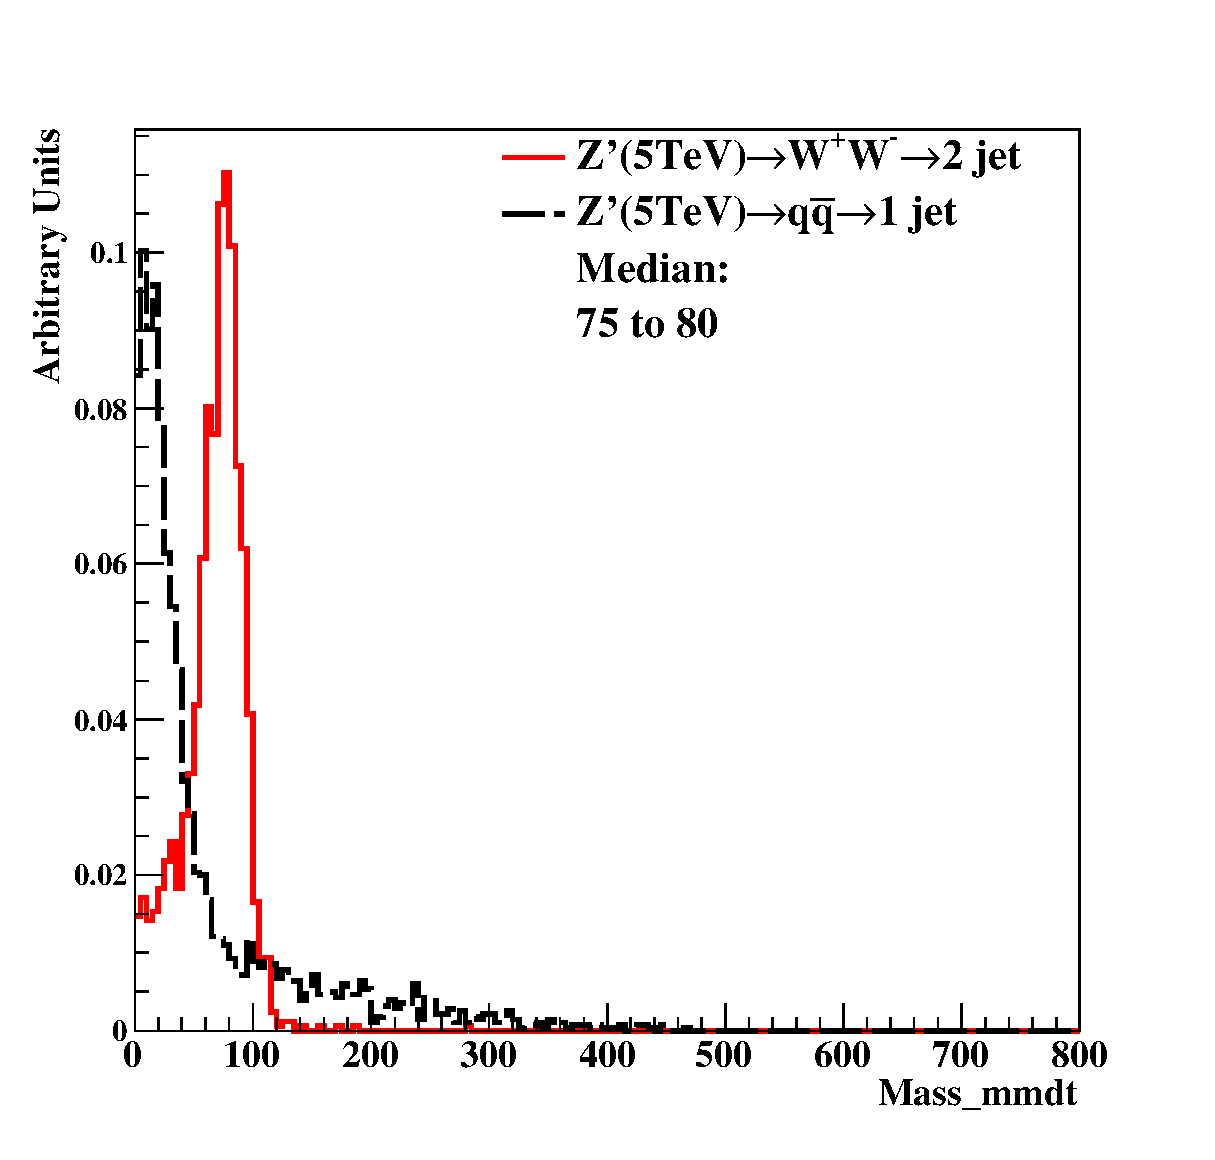
\includegraphics[width=0.43\textwidth]{figs/Dis_cluster_012_mass_mmdt_5tev_04.eps}
   }
   \subfigure[10TeV at 1$\times$1(cm$\times$cm) in cluster] {
   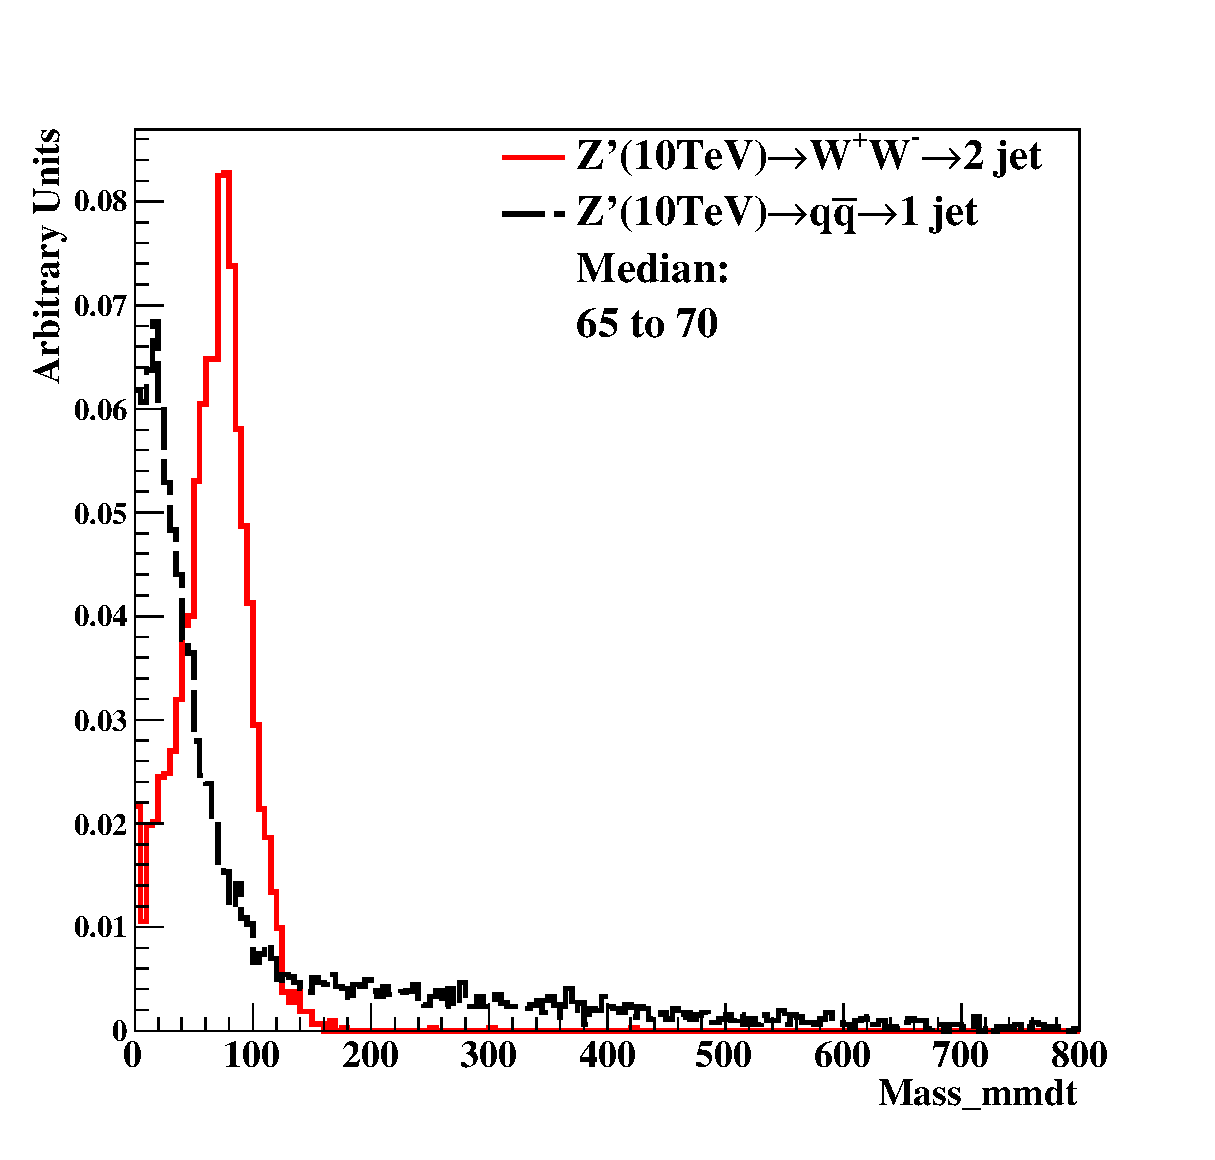
\includegraphics[width=0.43\textwidth]{figs/Dis_cluster_012_mass_mmdt_10tev_04.eps}
   }
\end{center}
\caption{Distributions of mass soft drop at $\beta$=0, signal=ww, in 5,10TeV energy of collision  in different detector sizes. Cell Size in 20$\times$20, 5$\times$5, and 1$\times$1(cm$\times$cm) are shown here.}
\label{fig:cluster_tau21_tau32}
\end{figure}

\begin{figure}
\begin{center}
   \subfigure[20TeV at 20$\times$20(cm$\times$cm) in cluster] {
   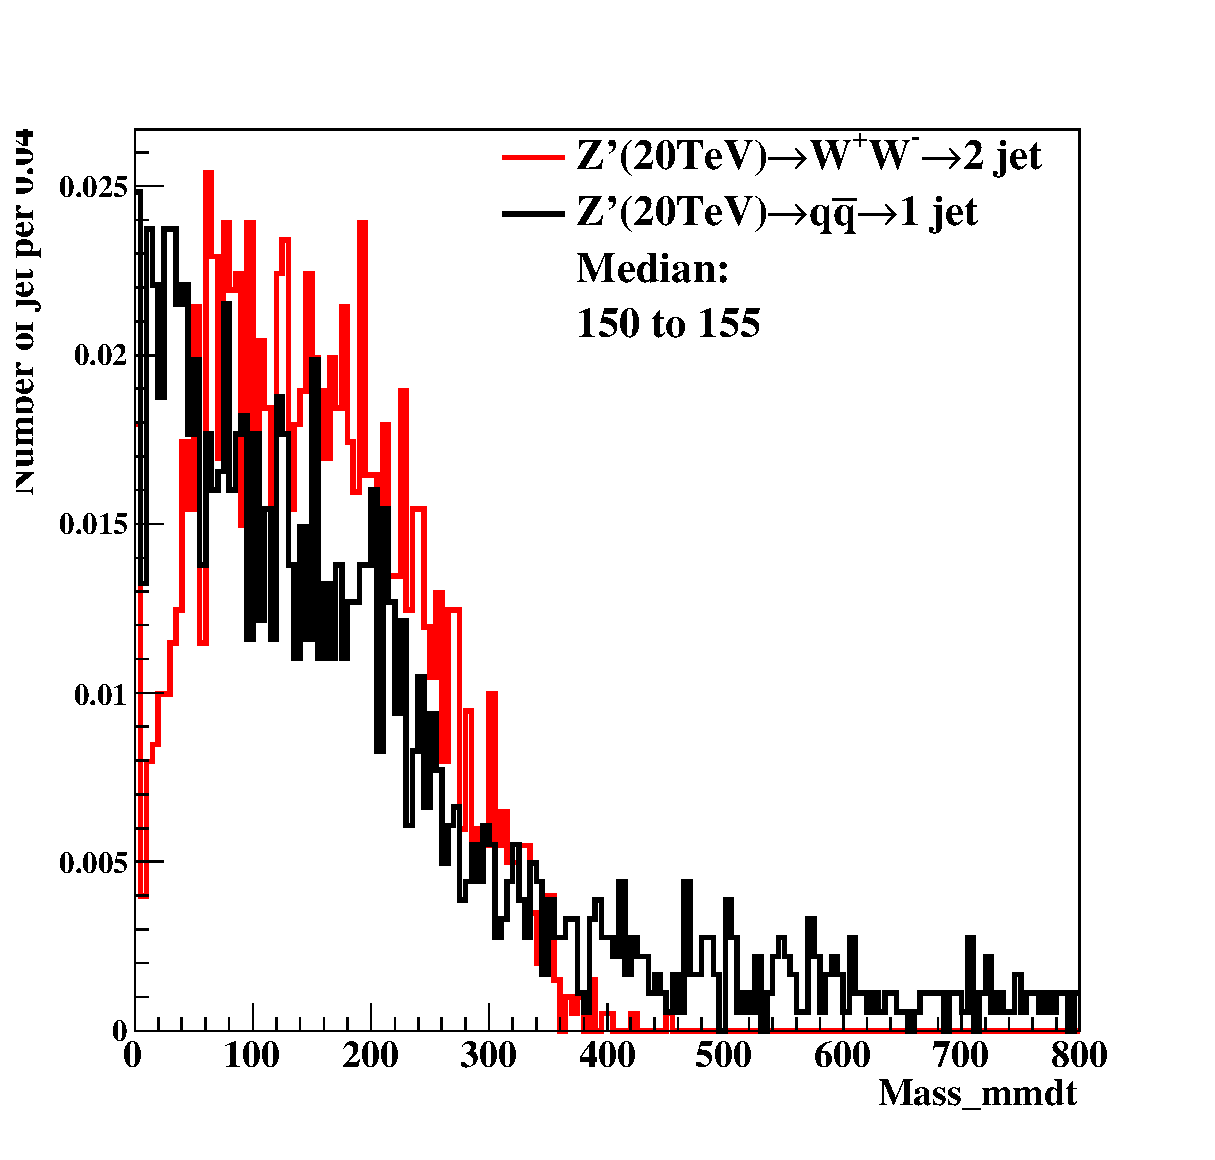
\includegraphics[width=0.43\textwidth]{figs/Dis_cluster_010_mass_mmdt_20tev_04.eps}\hfill
   }
      \subfigure[40TeV at 20$\times$20(cm$\times$cm) in cluster] {
   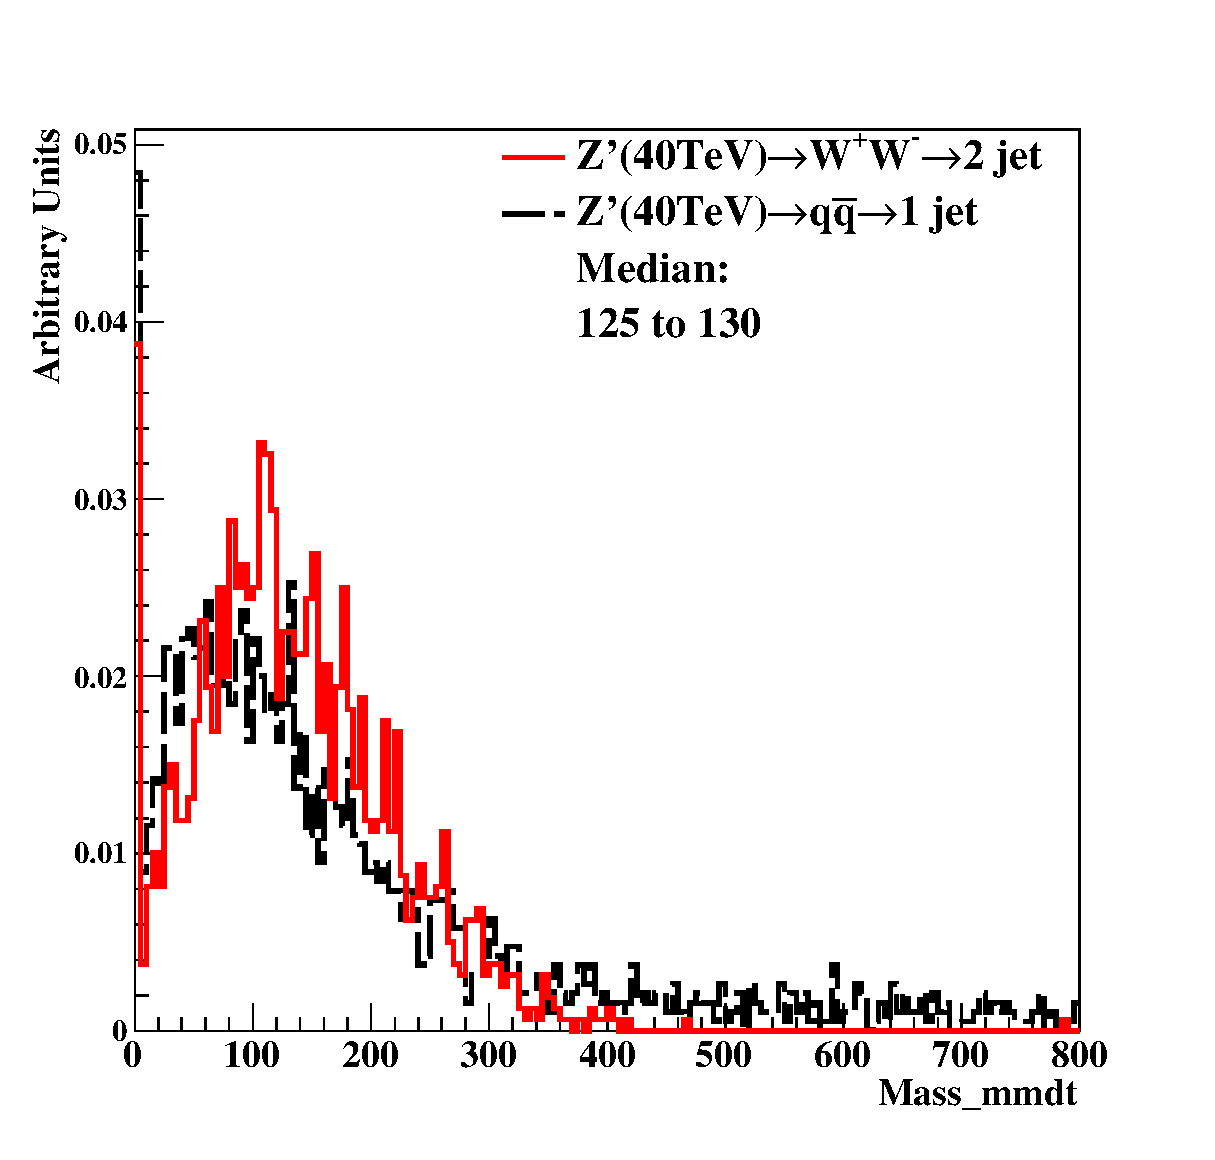
\includegraphics[width=0.43\textwidth]{figs/Dis_cluster_010_mass_mmdt_40tev_04.eps}\hfill
   }
   \subfigure[20TeV at 5$\times$5(cm$\times$cm) in cluster] {
   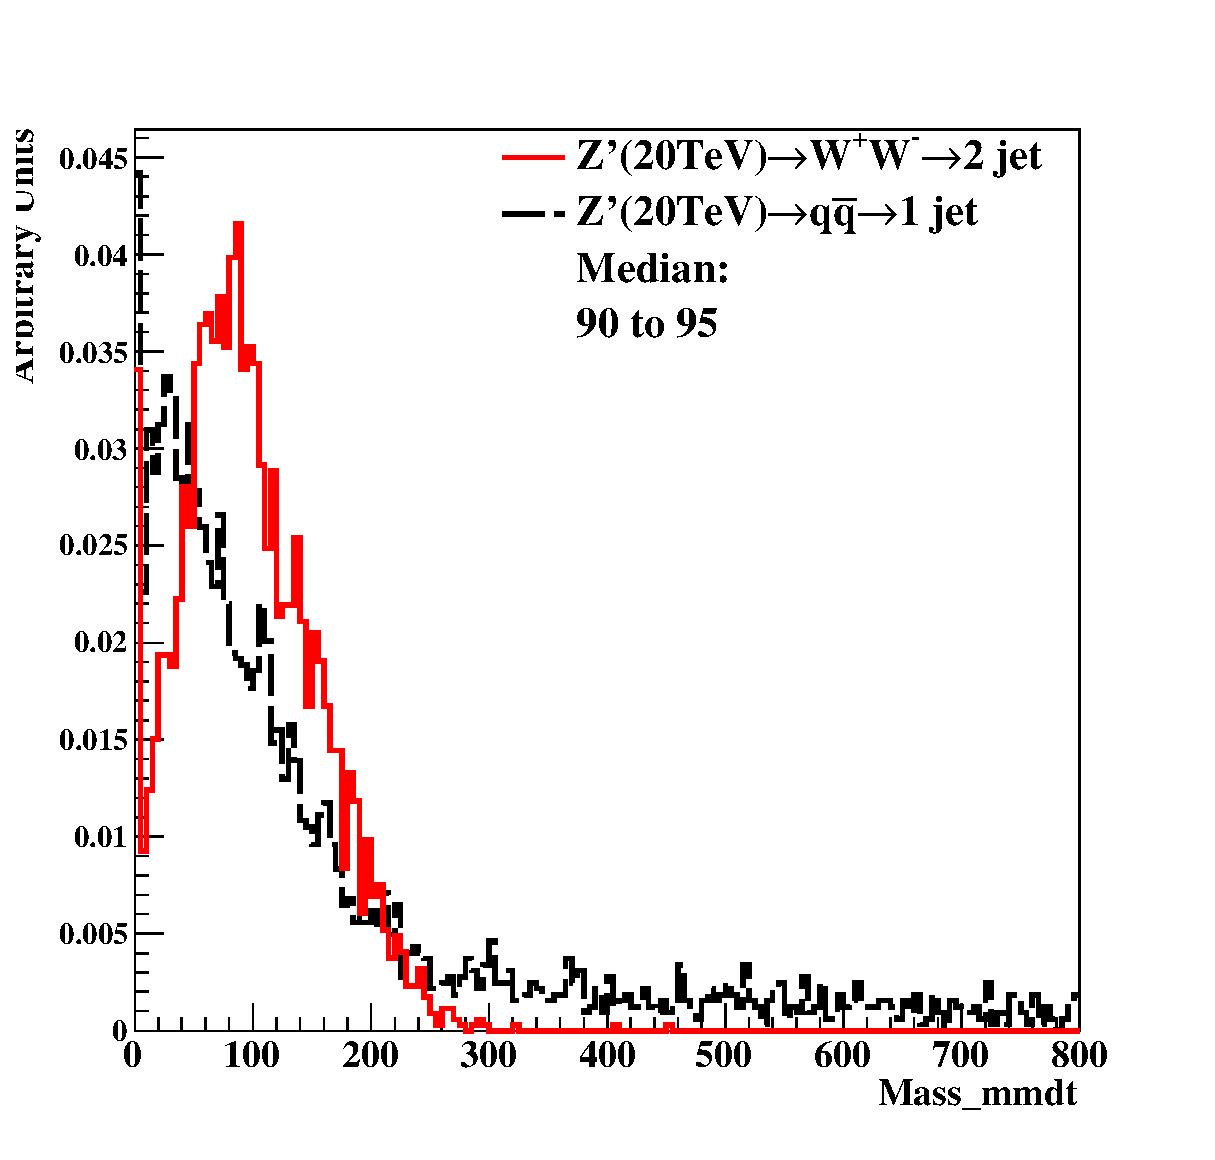
\includegraphics[width=0.43\textwidth]{figs/Dis_cluster_009_mass_mmdt_20tev_04.eps}\hfill
   }
    \subfigure[40TeV at 5$\times$5(cm$\times$cm) in cluster] {
   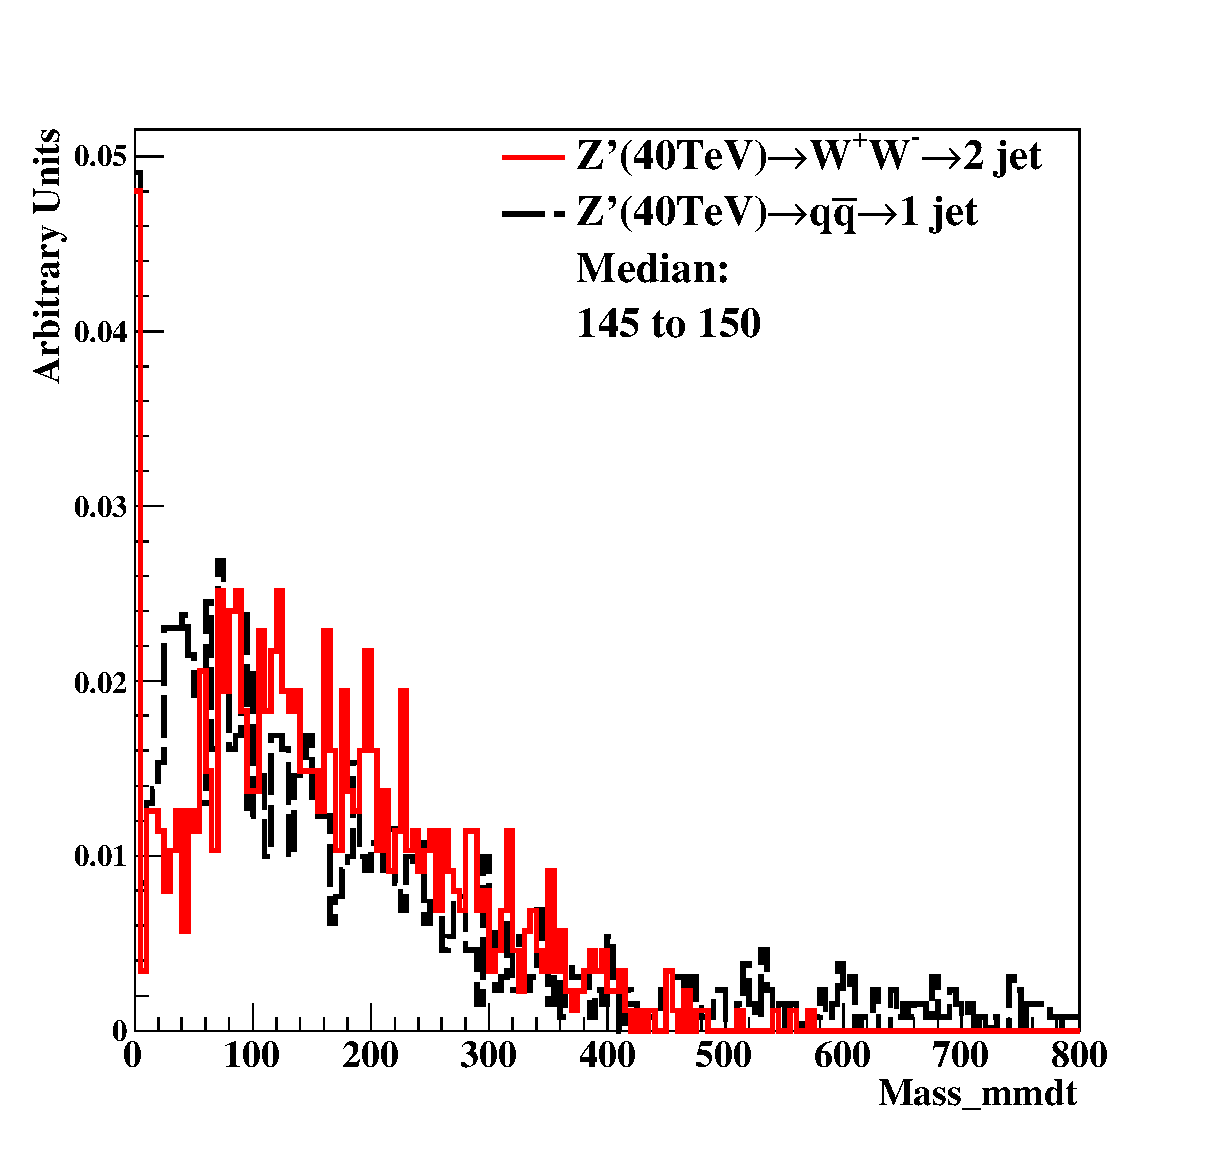
\includegraphics[width=0.43\textwidth]{figs/Dis_cluster_009_mass_mmdt_40tev_04.eps}
   }
   \subfigure[20TeV at 1$\times$1(cm$\times$cm) in cluster] {
   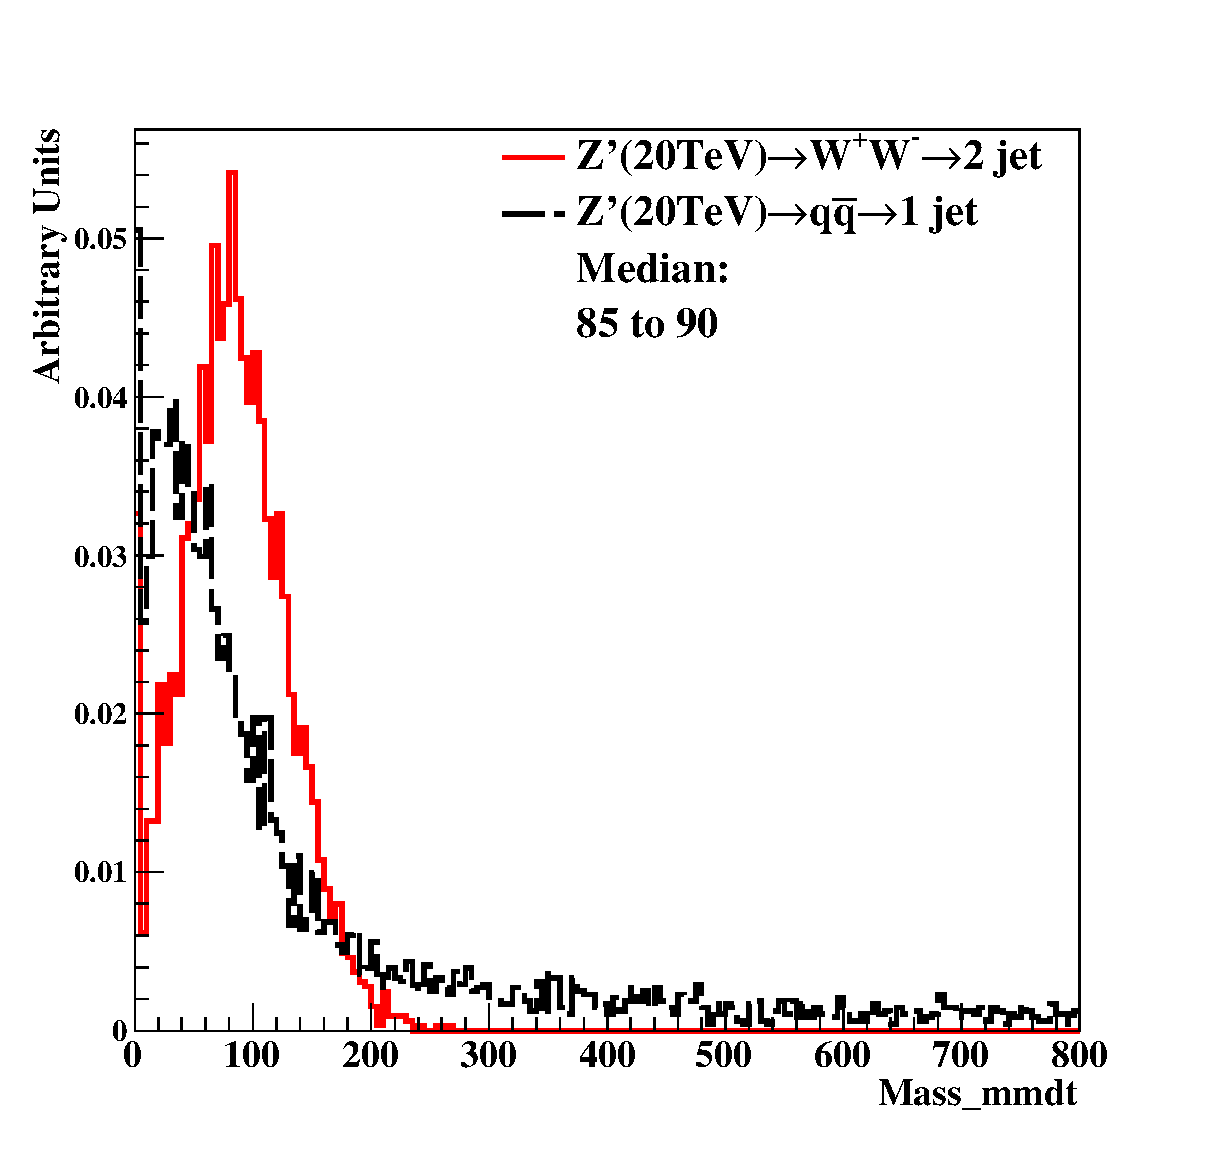
\includegraphics[width=0.43\textwidth]{figs/Dis_cluster_012_mass_mmdt_20tev_04.eps}\hfill
   }
      \subfigure[40TeV at 1$\times$1(cm$\times$cm) in cluster] {
   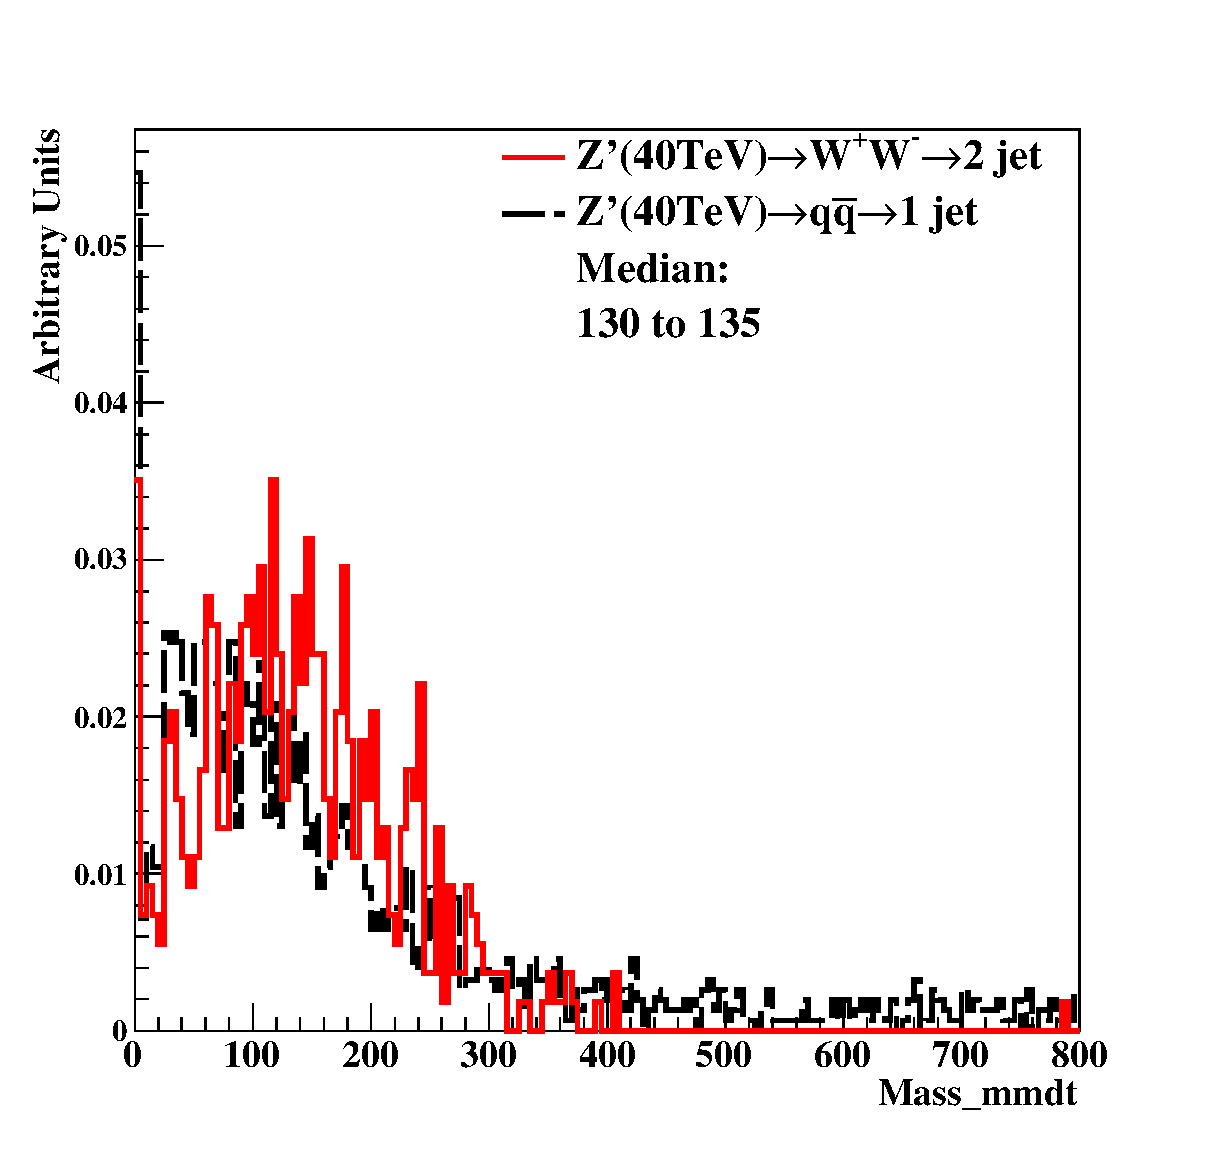
\includegraphics[width=0.43\textwidth]{figs/Dis_cluster_012_mass_mmdt_40tev_04.eps}
   }
\end{center}
\caption{Distributions of mass soft drop at $\beta$=0, signal=ww, in 20,40TeV energy of collision  in different detector sizes. Cell Size in 20$\times$20, 5$\times$5, and 1$\times$1(cm$\times$cm) are shown here.}
\label{fig:cluster_tau21_tau32}
\end{figure}

\begin{figure}
\begin{center}
  \subfigure[Central at Median($20\times20$=80,$5\times5$=80,$1\times1$=80) change width in cluster at 5TeV] {
  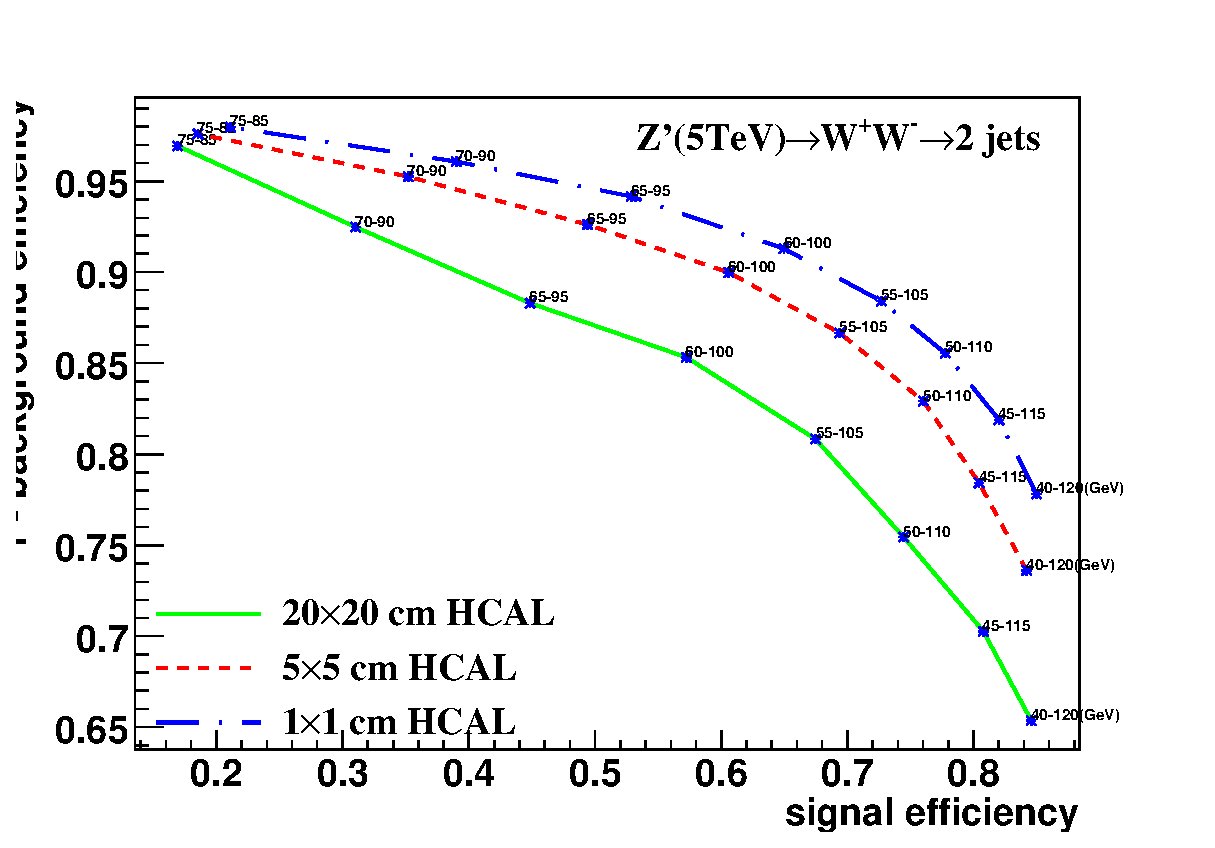
\includegraphics[width=0.43\textwidth]{figs/A_Cluster_mass_mmdt_5tev_eff_1_central_fix_ww_qq.eps}
  }
  \subfigure[Central at Median($20\times20$=95,$5\times5$=80,$1\times1$=75) change width in cluster at 10TeV] {
  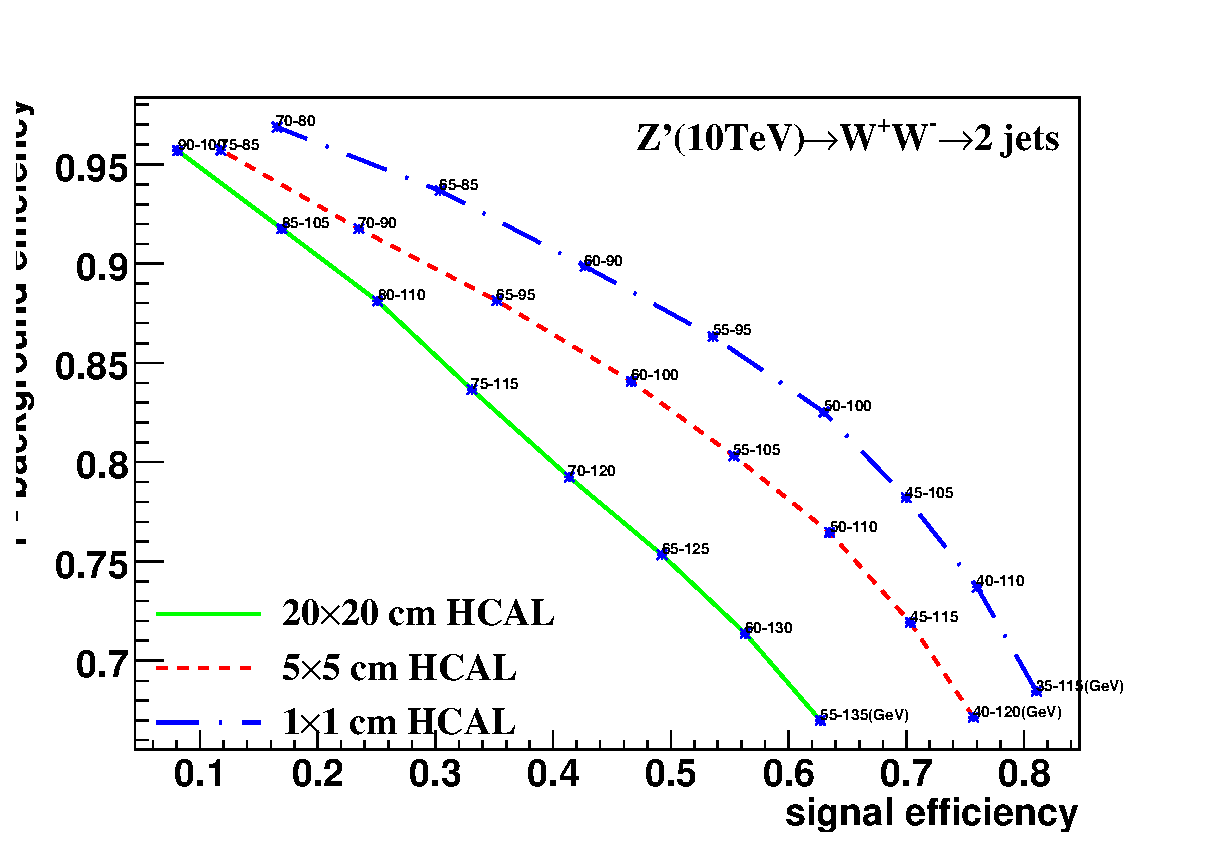
\includegraphics[width=0.43\textwidth]{figs/A_Cluster_mass_mmdt_10tev_eff_1_central_fix_ww_qq.eps}
  }
 \subfigure[Central at Median($20\times20$=155,$5\times5$=95,$1\times1$=90) change width in cluster at 20TeV] {
 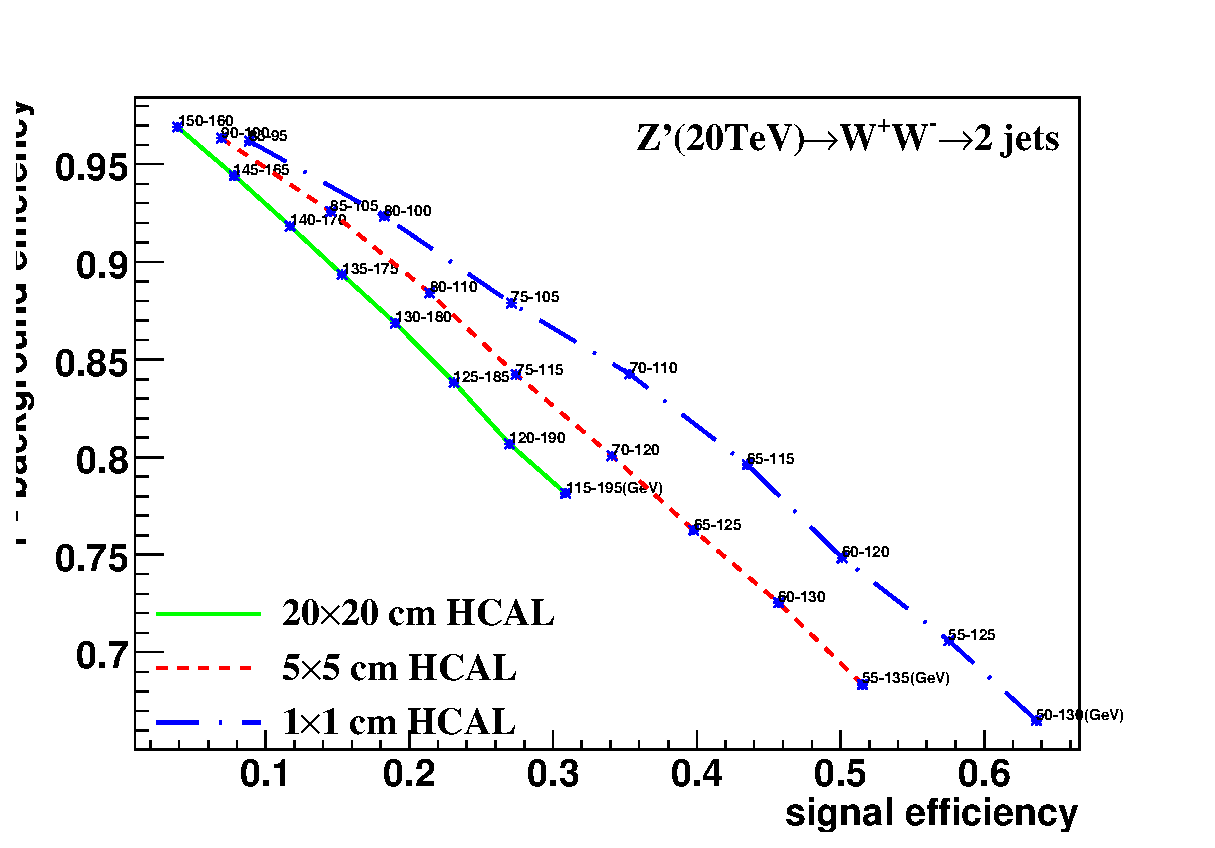
\includegraphics[width=0.43\textwidth]{figs/A_Cluster_mass_mmdt_20tev_eff_1_central_fix_ww_qq.eps}
 }
 \subfigure[Central at Median($20\times20$=130,$5\times5$=150,$1\times1$=135) change width in cluster at 40TeV] {
 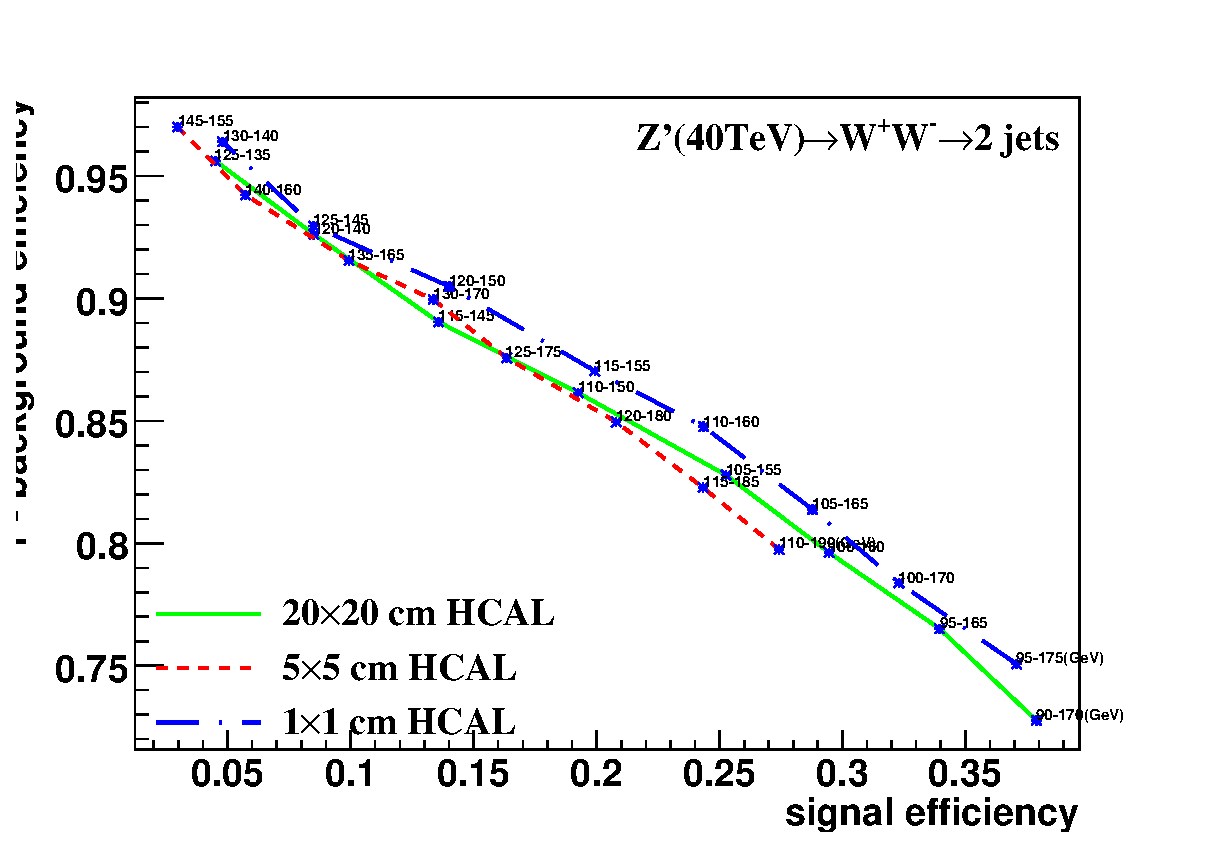
\includegraphics[width=0.43\textwidth]{figs/A_Cluster_mass_mmdt_40tev_eff_1_central_fix_ww_qq.eps}
 }
\end{center}
\caption{study of "fix central and change width" in mass soft drop at $\beta$=0, signal=ww, in 5, 10, 20, 40TeV energy of collision  in different detector sizes. Cell Size in 20$\times$20, 5$\times$5, and 1$\times$1(cm$\times$cm) are shown in each picture.}
\label{fig:cluster_tau21_tau32}
\end{figure}

\begin{figure}
\begin{center}
  \subfigure[Central at Median($20\times20$=80,$5\times5$=80,$1\times1$=80) change width in cluster at 5TeV] {
  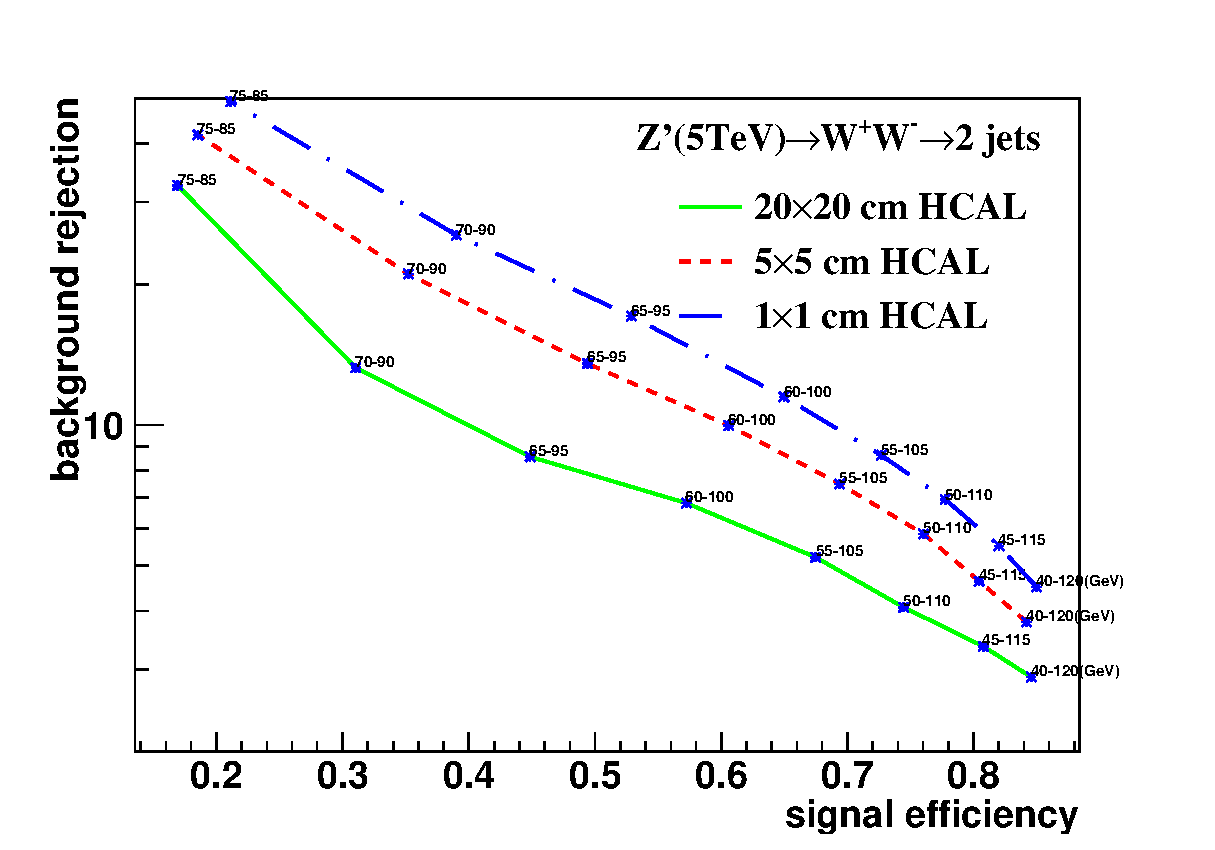
\includegraphics[width=0.43\textwidth]{figs/A_Cluster_mass_mmdt_5tev_eff_1_central_fix_ww_qq_log.eps}
  }
  \subfigure[Central at Median($20\times20$=95,$5\times5$=80,$1\times1$=75) change width in cluster at 10TeV] {
  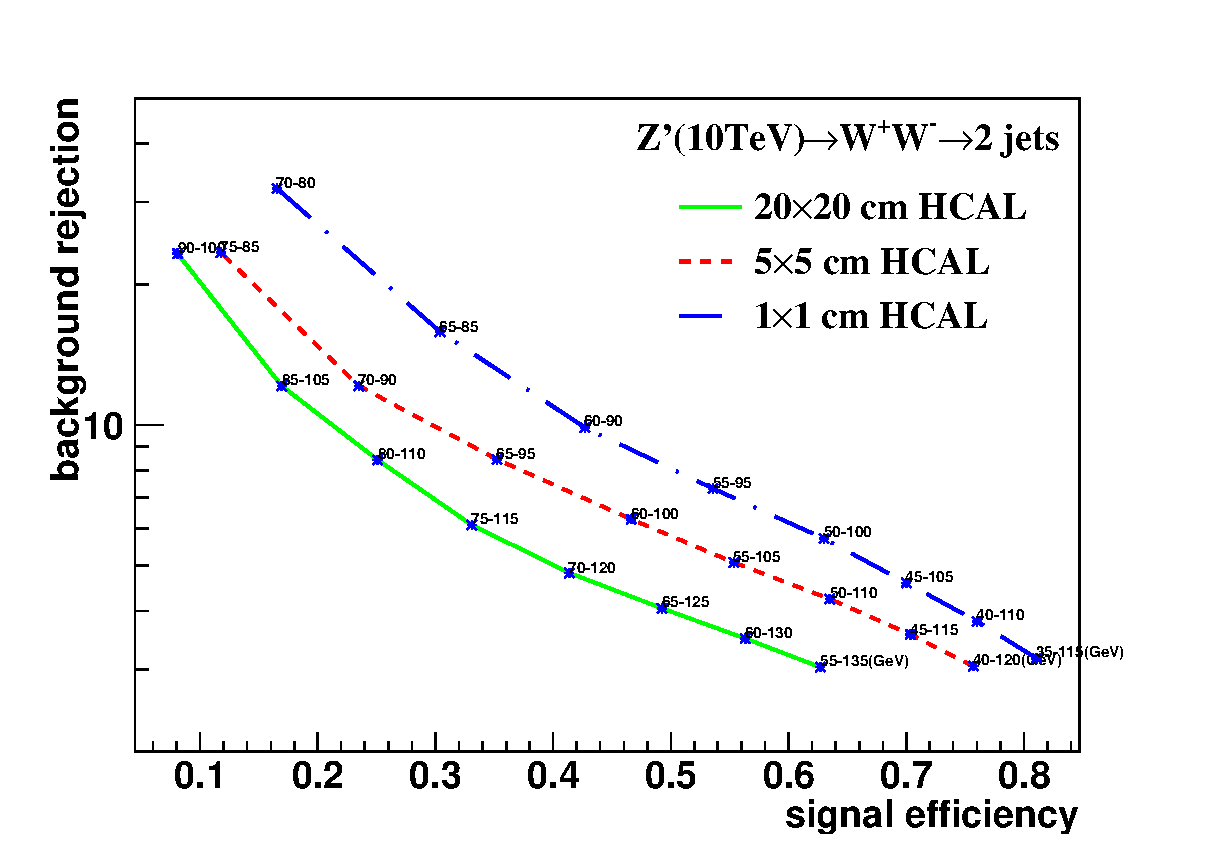
\includegraphics[width=0.43\textwidth]{figs/A_Cluster_mass_mmdt_10tev_eff_1_central_fix_ww_qq_log.eps}
  }
 \subfigure[Central at Median($20\times20$=155,$5\times5$=95,$1\times1$=90) change width in cluster at 20TeV] {
 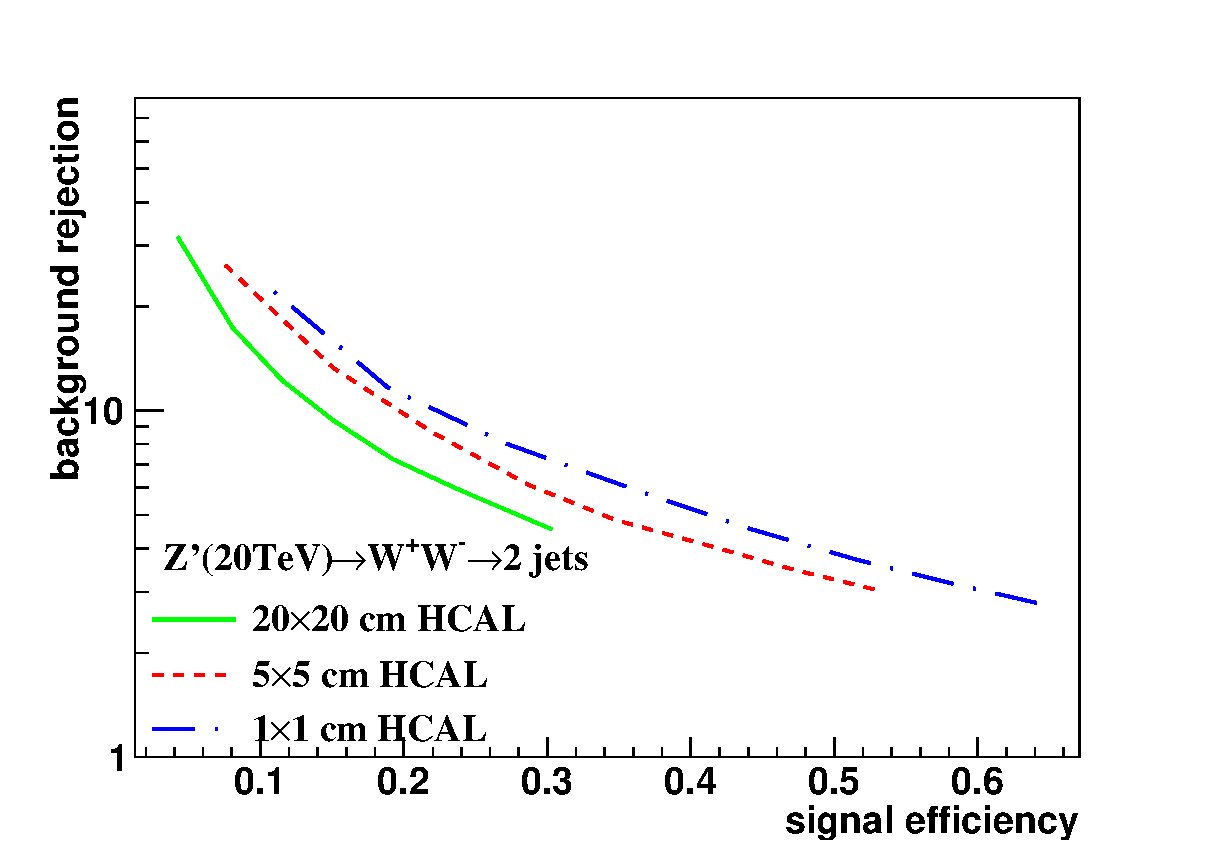
\includegraphics[width=0.43\textwidth]{figs/A_Cluster_mass_mmdt_20tev_eff_1_central_fix_ww_qq_log.eps}
 }
 \subfigure[Central at Median($20\times20$=130,$5\times5$=150,$1\times1$=135) change width in cluster at 40TeV] {
 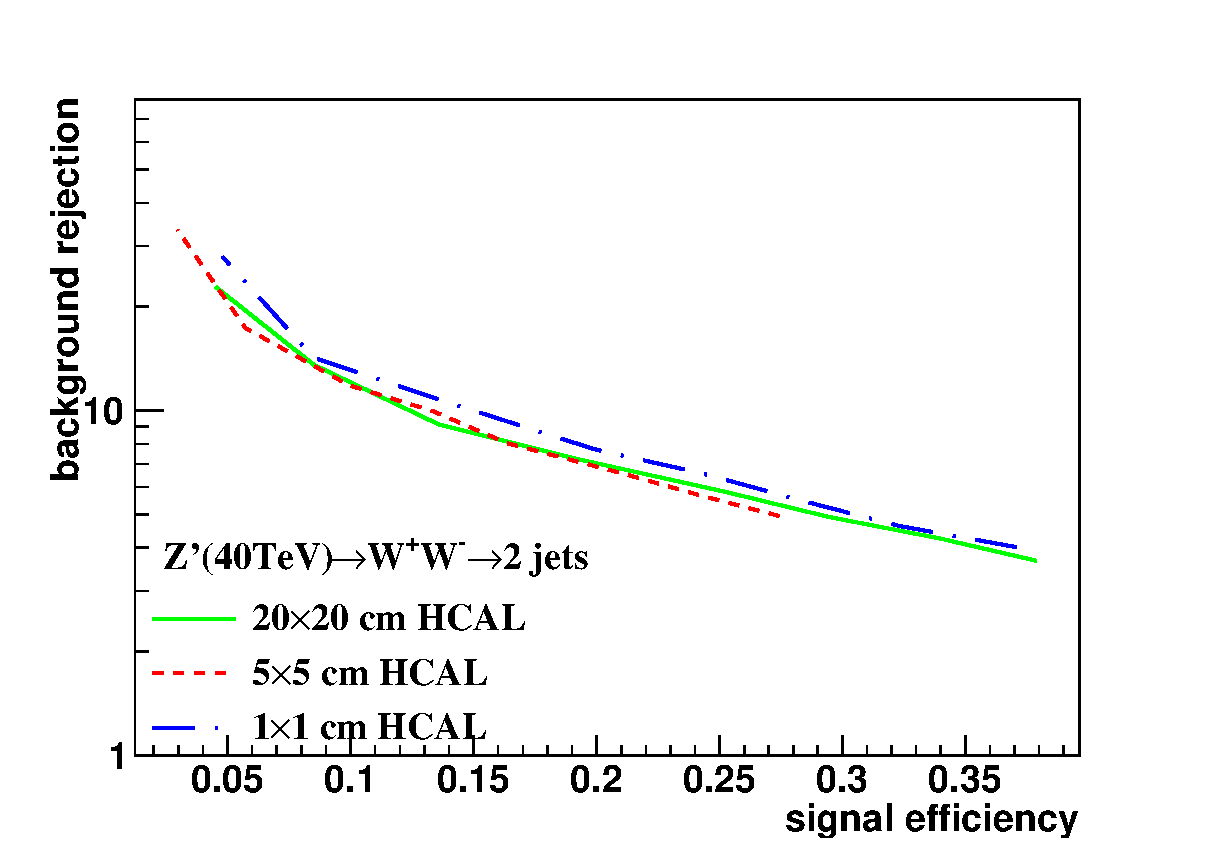
\includegraphics[width=0.43\textwidth]{figs/A_Cluster_mass_mmdt_40tev_eff_1_central_fix_ww_qq_log.eps}
 }
\end{center}
\caption{study of "fix central and change width" in mass soft drop at $\beta$=0, signal=ww, in 5, 10, 20, 40TeV energy of collision  in different detector sizes. Cell Size in 20$\times$20, 5$\times$5, and 1$\times$1(cm$\times$cm) are shown in each picture.}
\label{fig:cluster_tau21_tau32}
\end{figure}

\begin{figure}
\begin{center}
   \subfigure[5TeV at 20$\times$20(cm$\times$cm) in cluster] {
   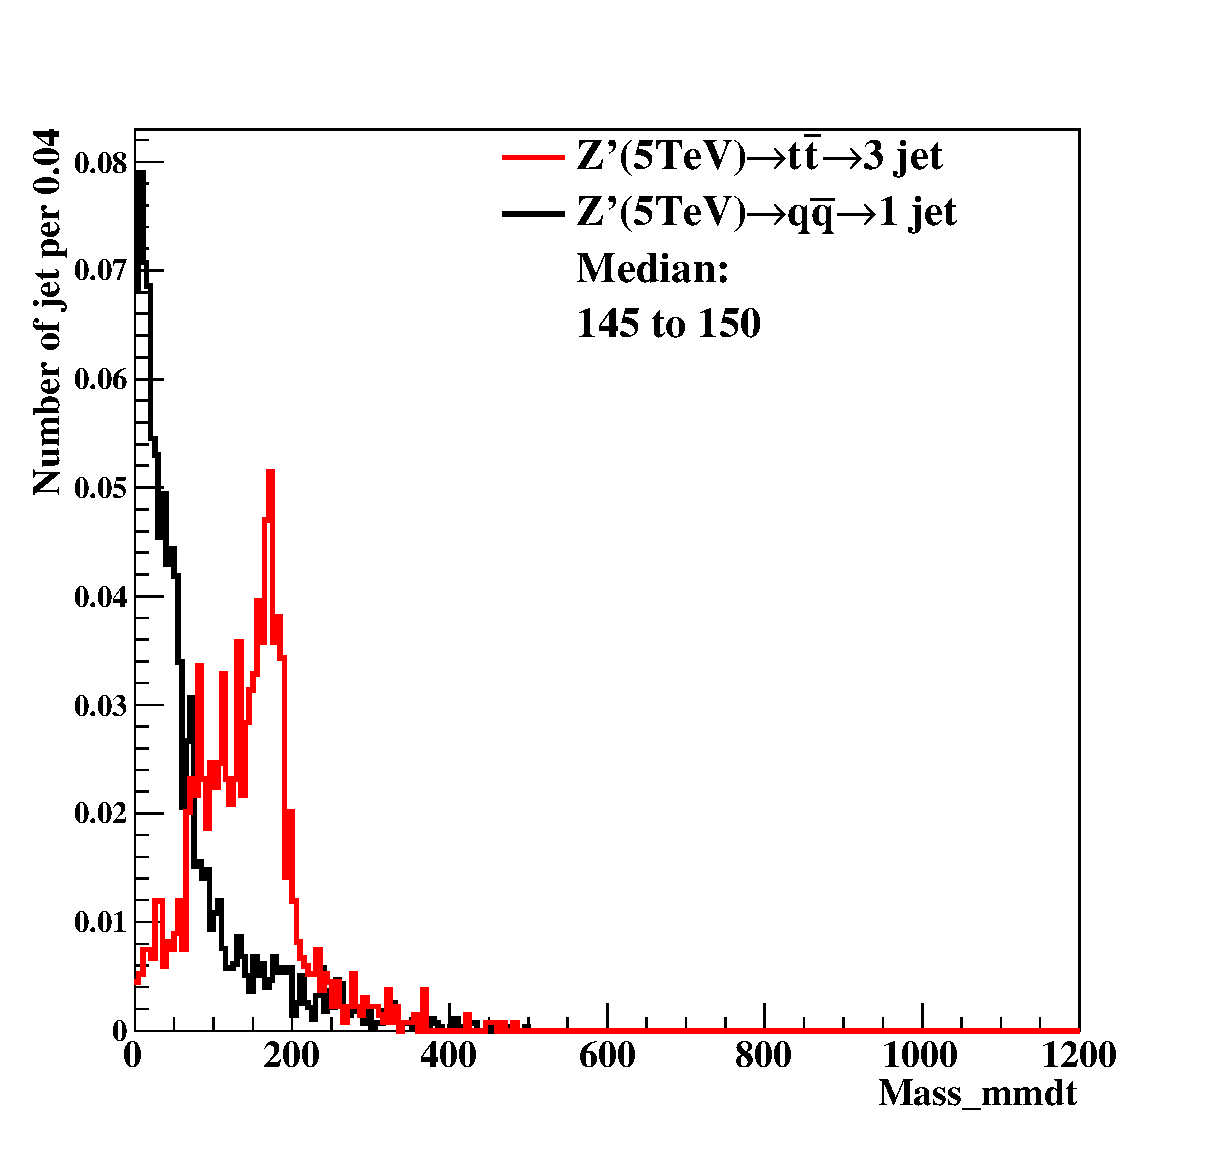
\includegraphics[width=0.43\textwidth]{figs/Dis_cluster_010_mass_mmdt_tt_5tev_04_tt.eps}
   }
      \subfigure[10TeV at 20$\times$20(cm$\times$cm) in cluster] {
   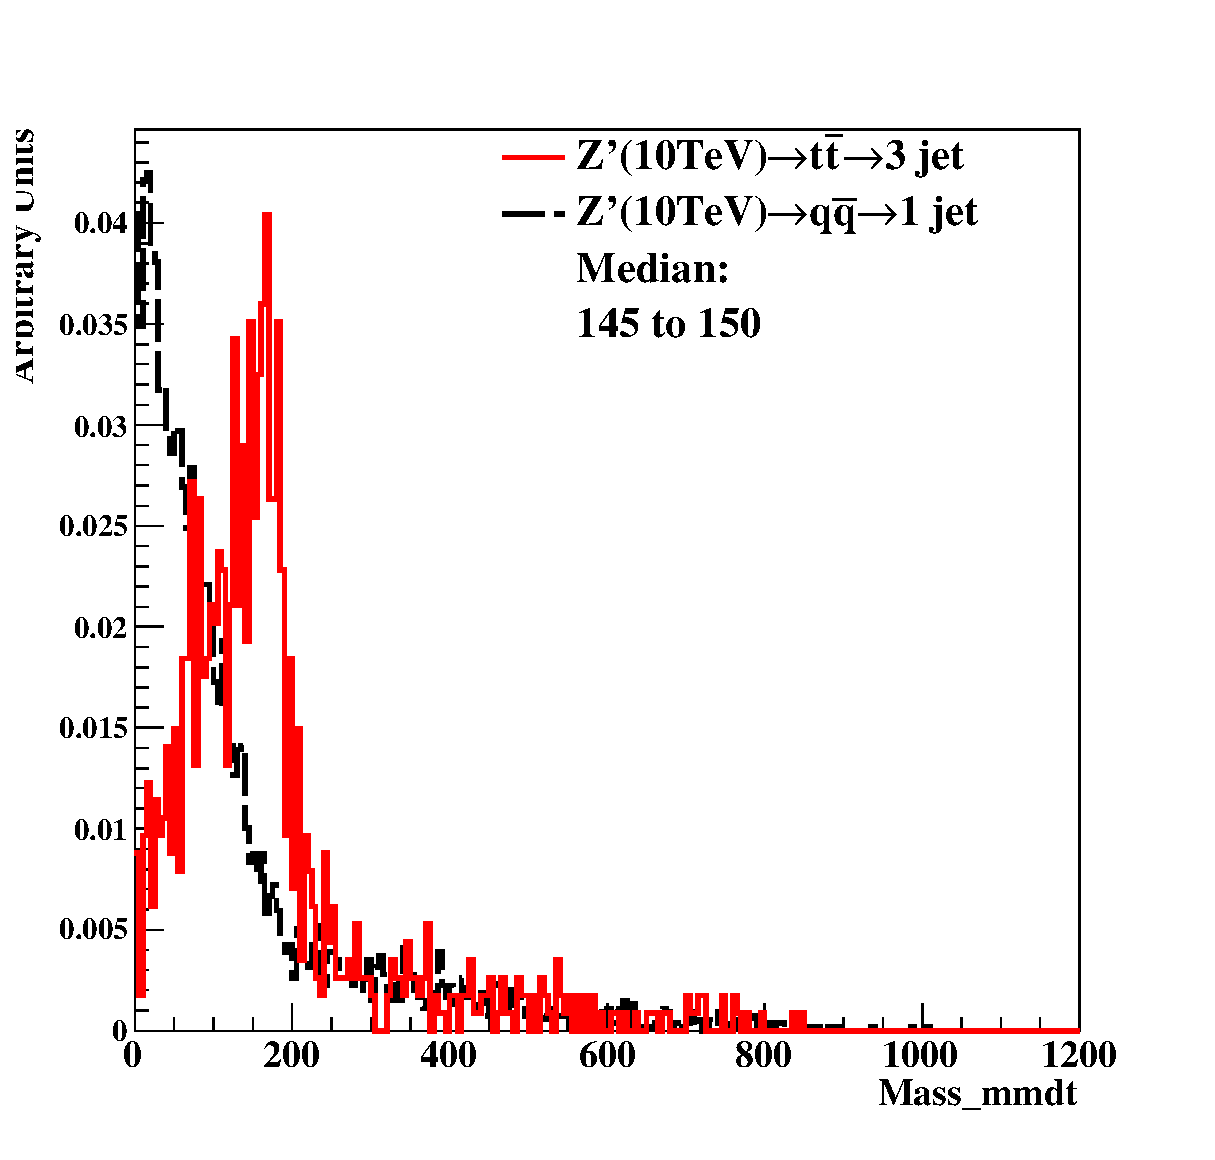
\includegraphics[width=0.43\textwidth]{figs/Dis_cluster_010_mass_mmdt_tt_10tev_04_tt.eps}
   }
   \subfigure[5TeV at 5$\times$5(cm$\times$cm) in cluster] {
   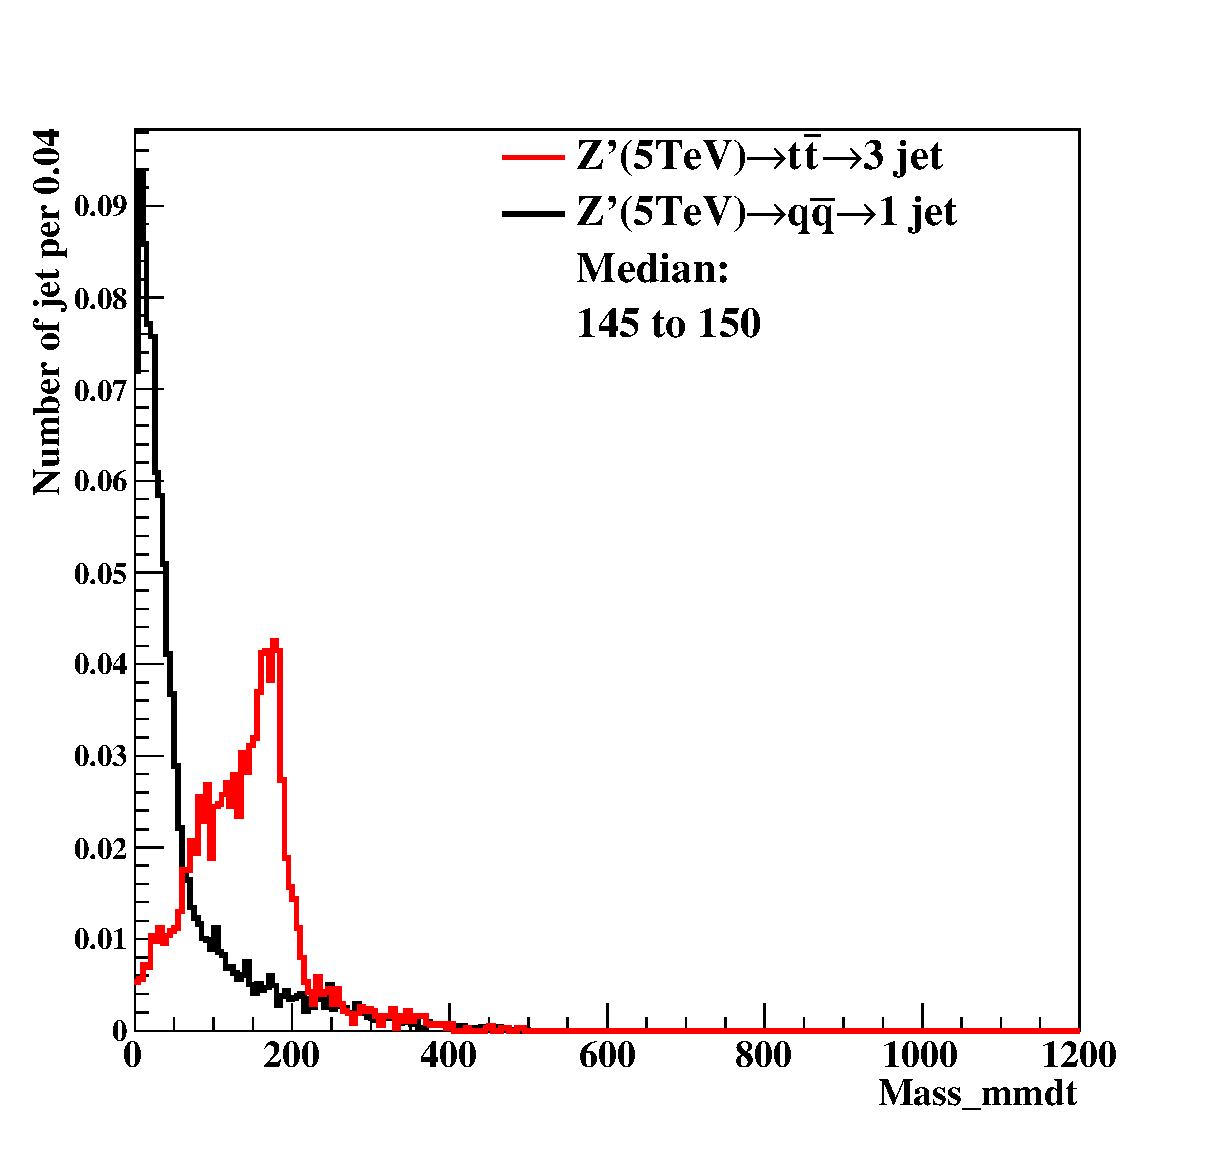
\includegraphics[width=0.43\textwidth]{figs/Dis_cluster_009_mass_mmdt_tt_5tev_04_tt.eps}
   }
    \subfigure[10TeV at 5$\times$5(cm$\times$cm) in cluster] {
   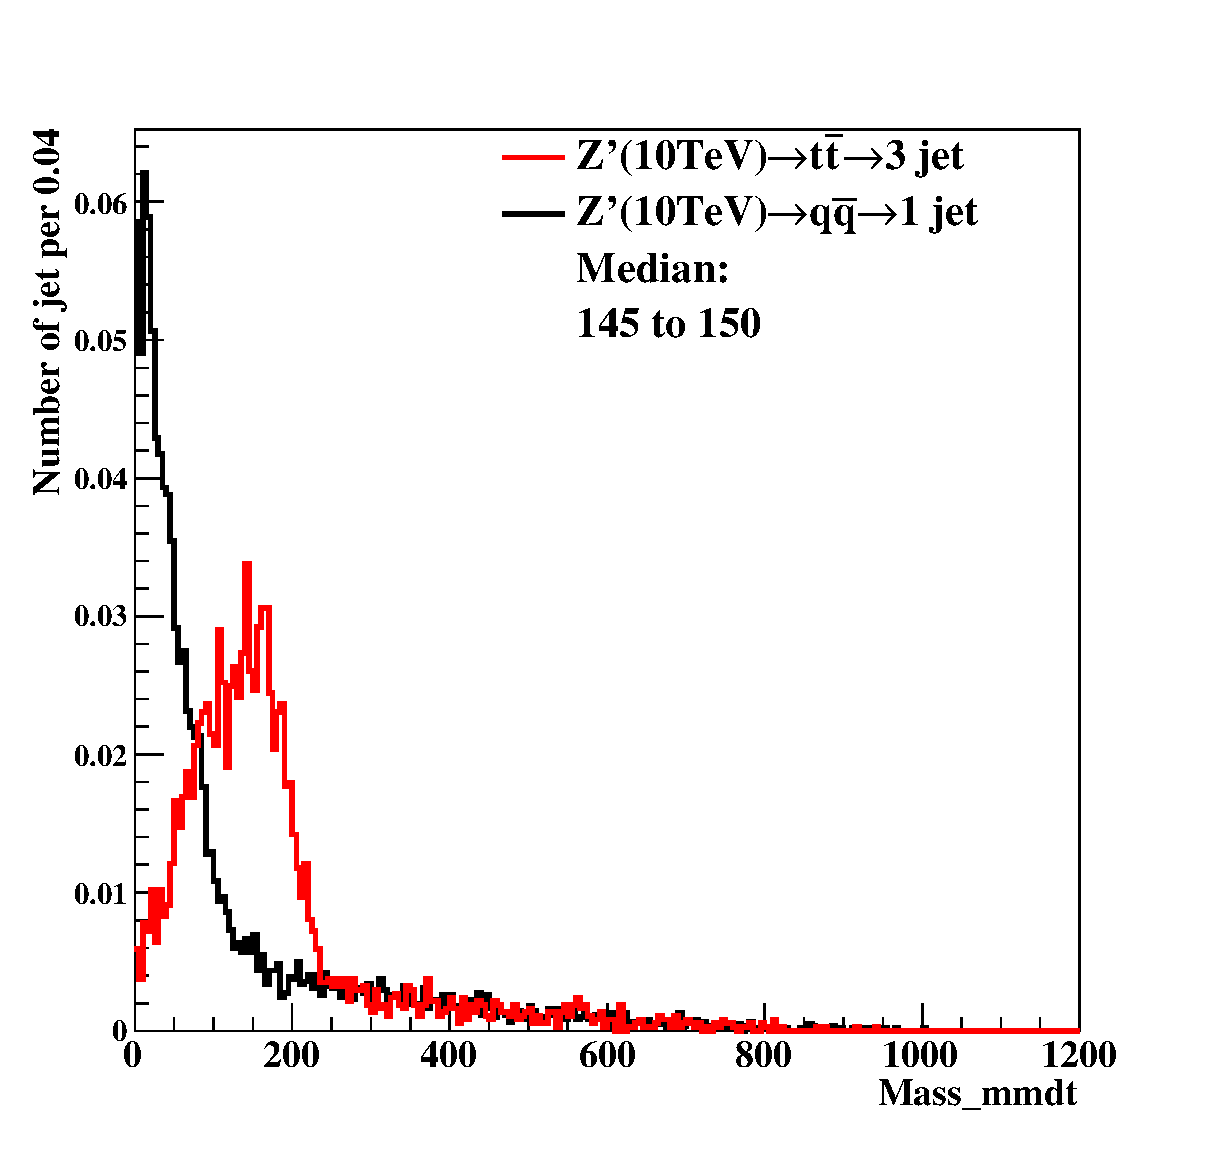
\includegraphics[width=0.43\textwidth]{figs/Dis_cluster_009_mass_mmdt_tt_10tev_04_tt.eps}
   }
   \subfigure[5TeV at 1$\times$1(cm$\times$cm) in cluster] {
   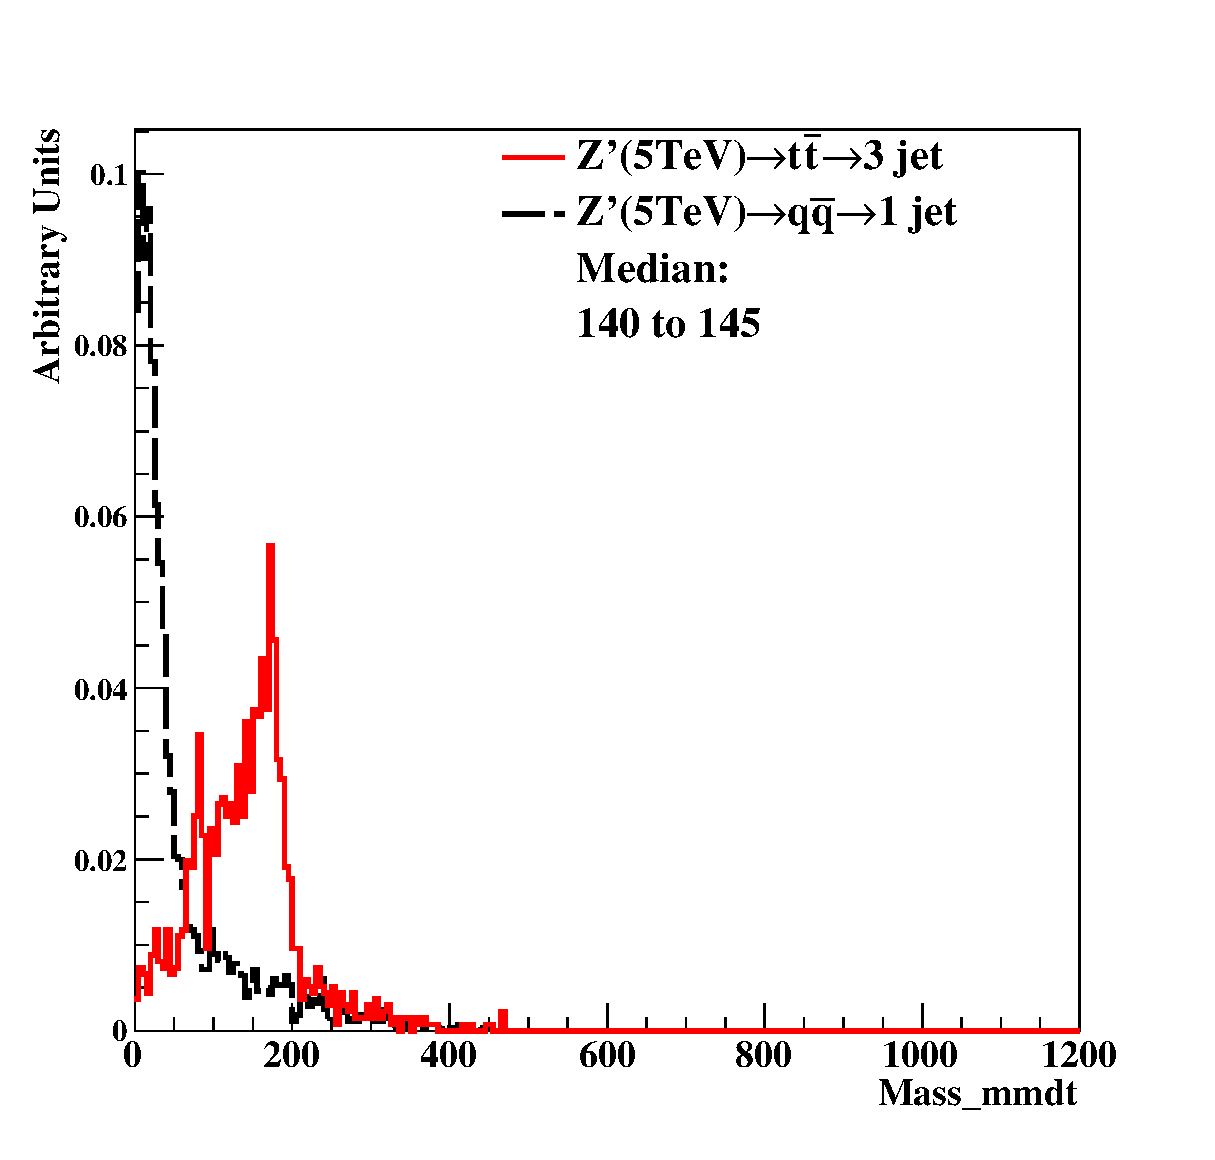
\includegraphics[width=0.43\textwidth]{figs/Dis_cluster_012_mass_mmdt_tt_5tev_04_tt.eps}
   }
   \subfigure[10TeV at 1$\times$1(cm$\times$cm) in cluster] {
   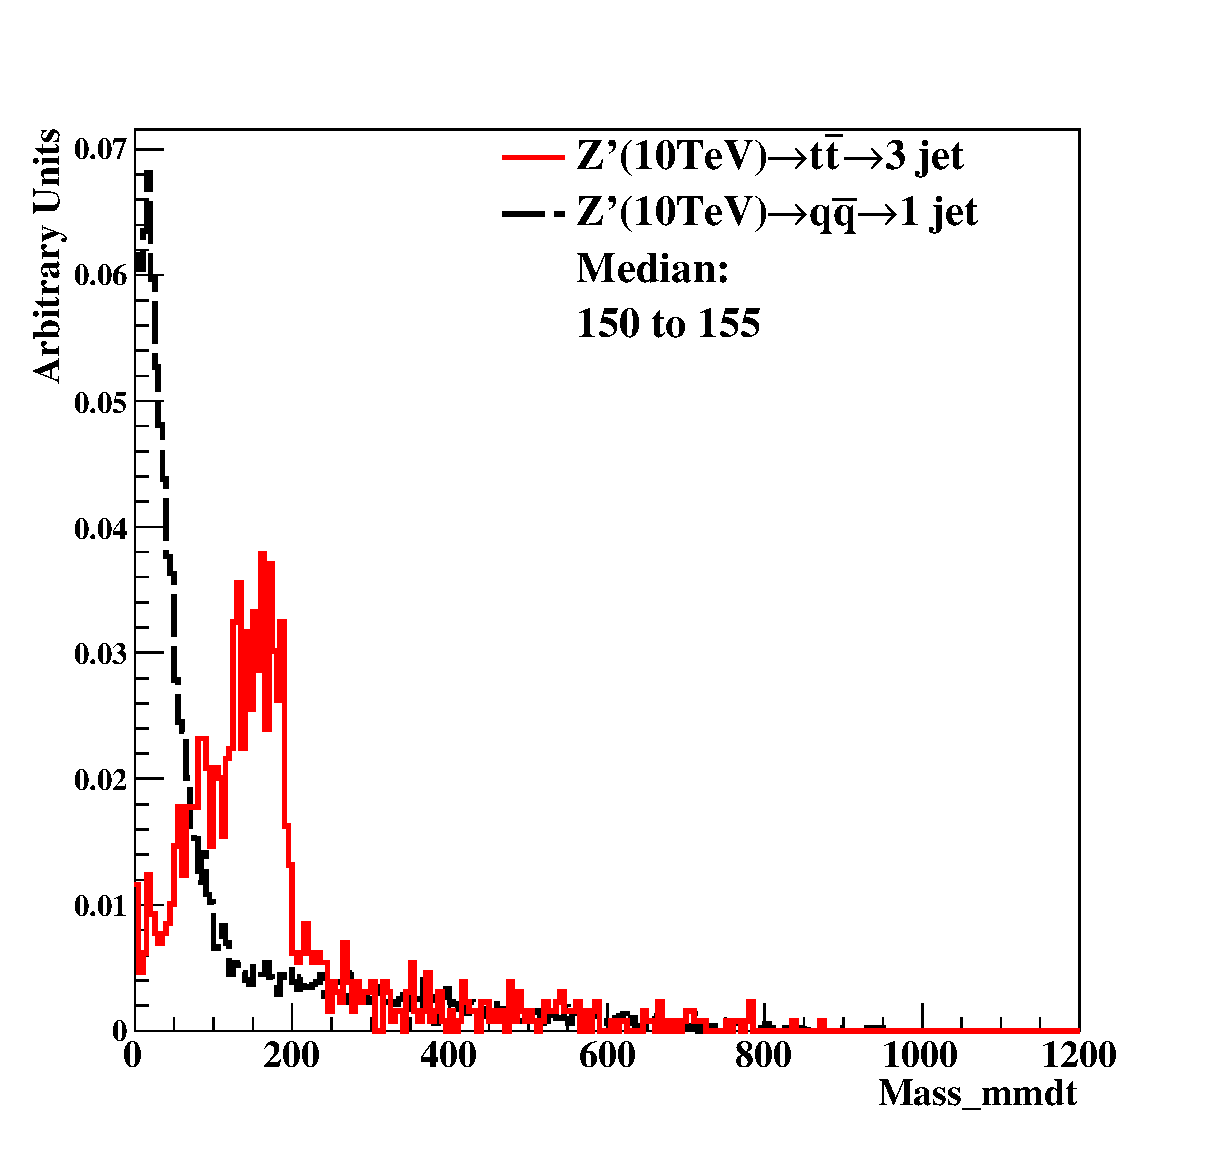
\includegraphics[width=0.43\textwidth]{figs/Dis_cluster_012_mass_mmdt_tt_10tev_04_tt.eps}
   }
\end{center}
\caption{Distributions of mass soft drop at $\beta$=0, signal=tt, in 5,10TeV energy of collision  in different detector sizes. Cell Size in 20$\times$20, 5$\times$5, and 1$\times$1(cm$\times$cm) are shown here.}
\label{fig:cluster_tau21_tau32}
\end{figure}

\begin{figure}
\begin{center}
   \subfigure[20TeV at 20$\times$20(cm$\times$cm) in cluster] {
   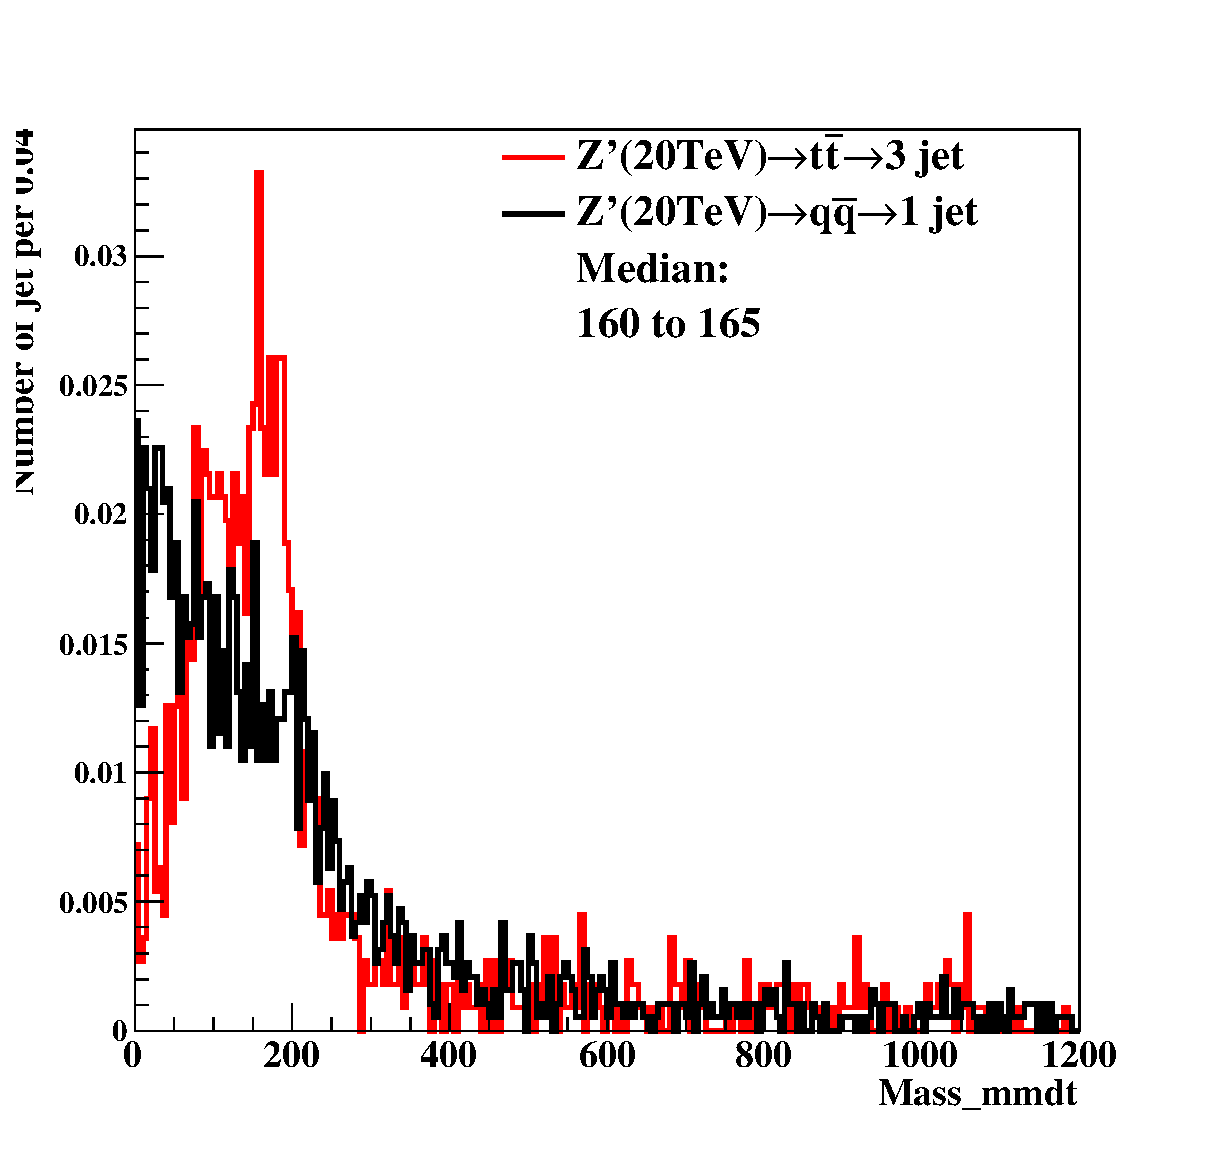
\includegraphics[width=0.43\textwidth]{figs/Dis_cluster_010_mass_mmdt_tt_20tev_04_tt.eps}\hfill
   }
      \subfigure[40TeV at 20$\times$20(cm$\times$cm) in cluster] {
   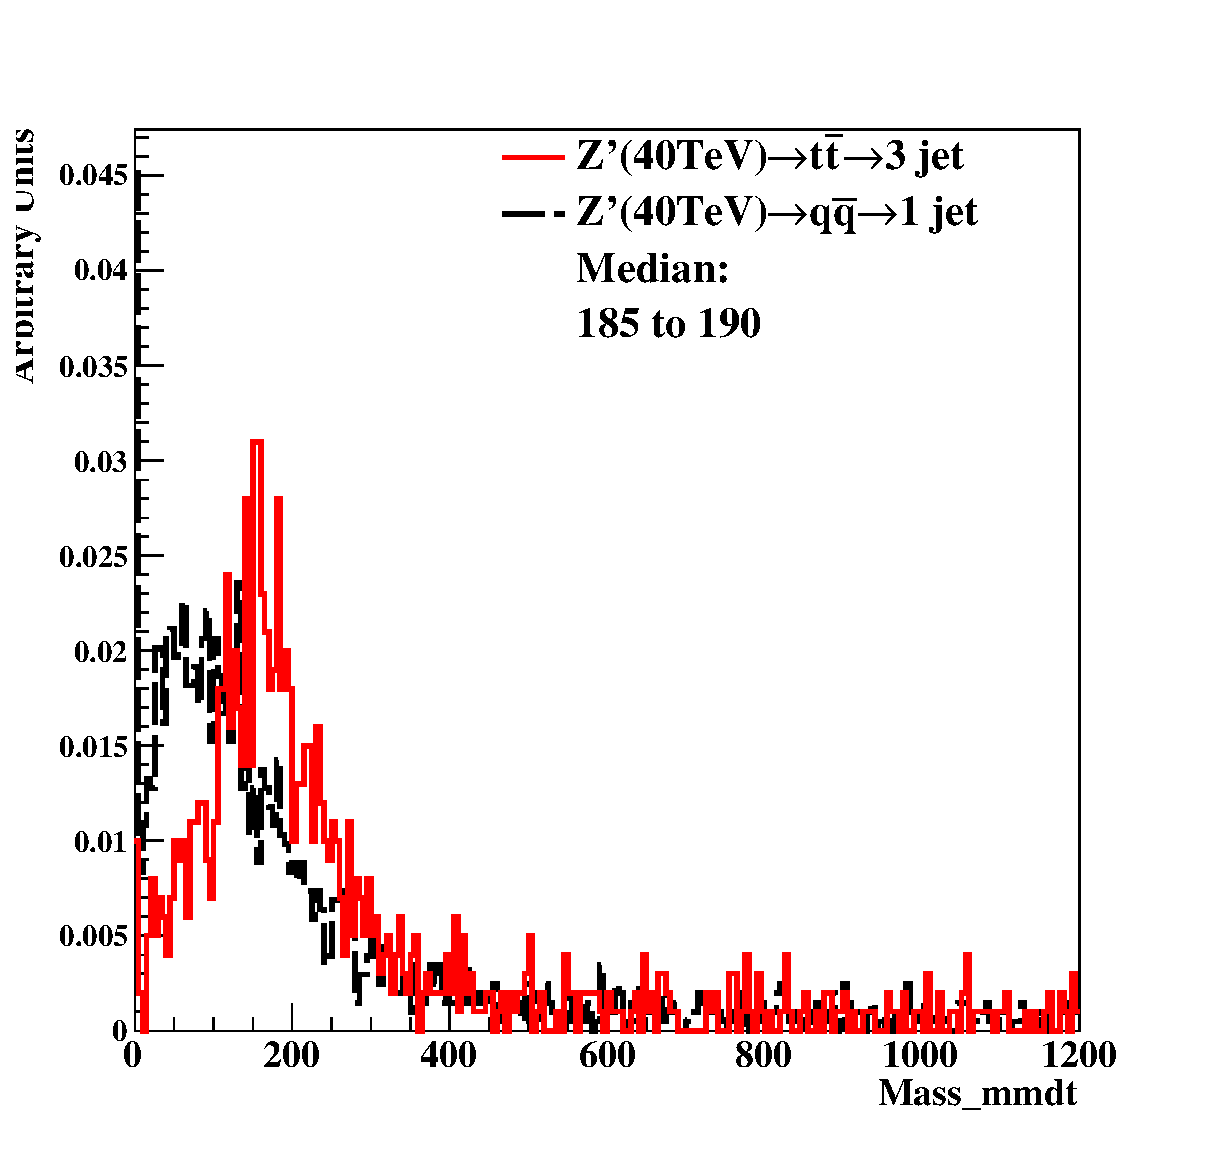
\includegraphics[width=0.43\textwidth]{figs/Dis_cluster_010_mass_mmdt_tt_40tev_04_tt.eps}\hfill
   }
   \subfigure[20TeV at 5$\times$5(cm$\times$cm) in cluster] {
   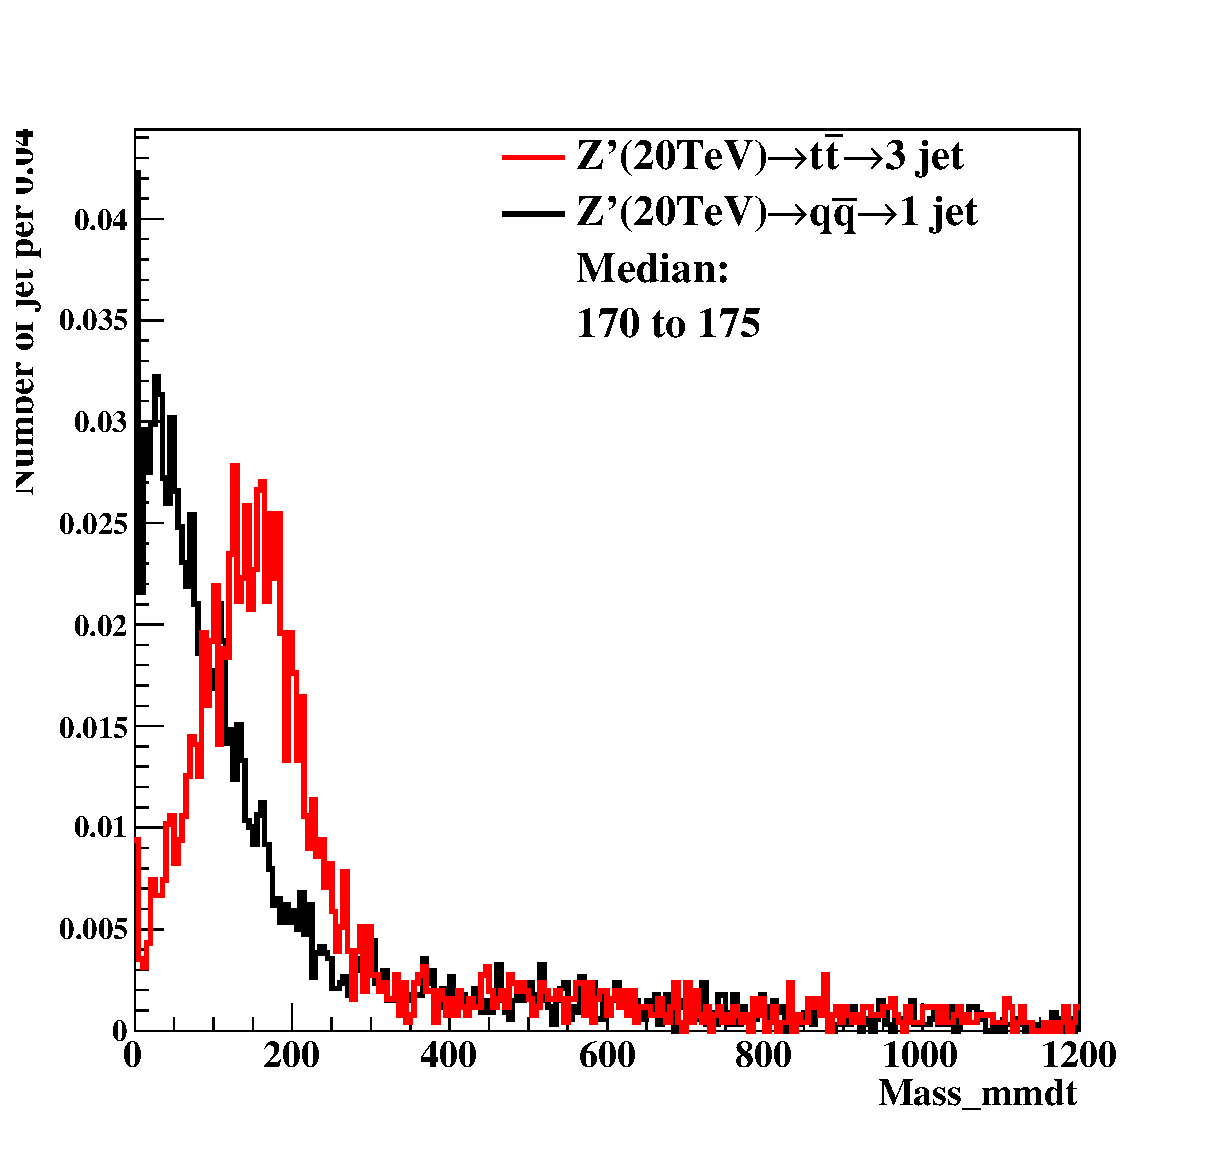
\includegraphics[width=0.43\textwidth]{figs/Dis_cluster_009_mass_mmdt_tt_20tev_04_tt.eps}\hfill
   }
    \subfigure[40TeV at 5$\times$5(cm$\times$cm) in cluster] {
   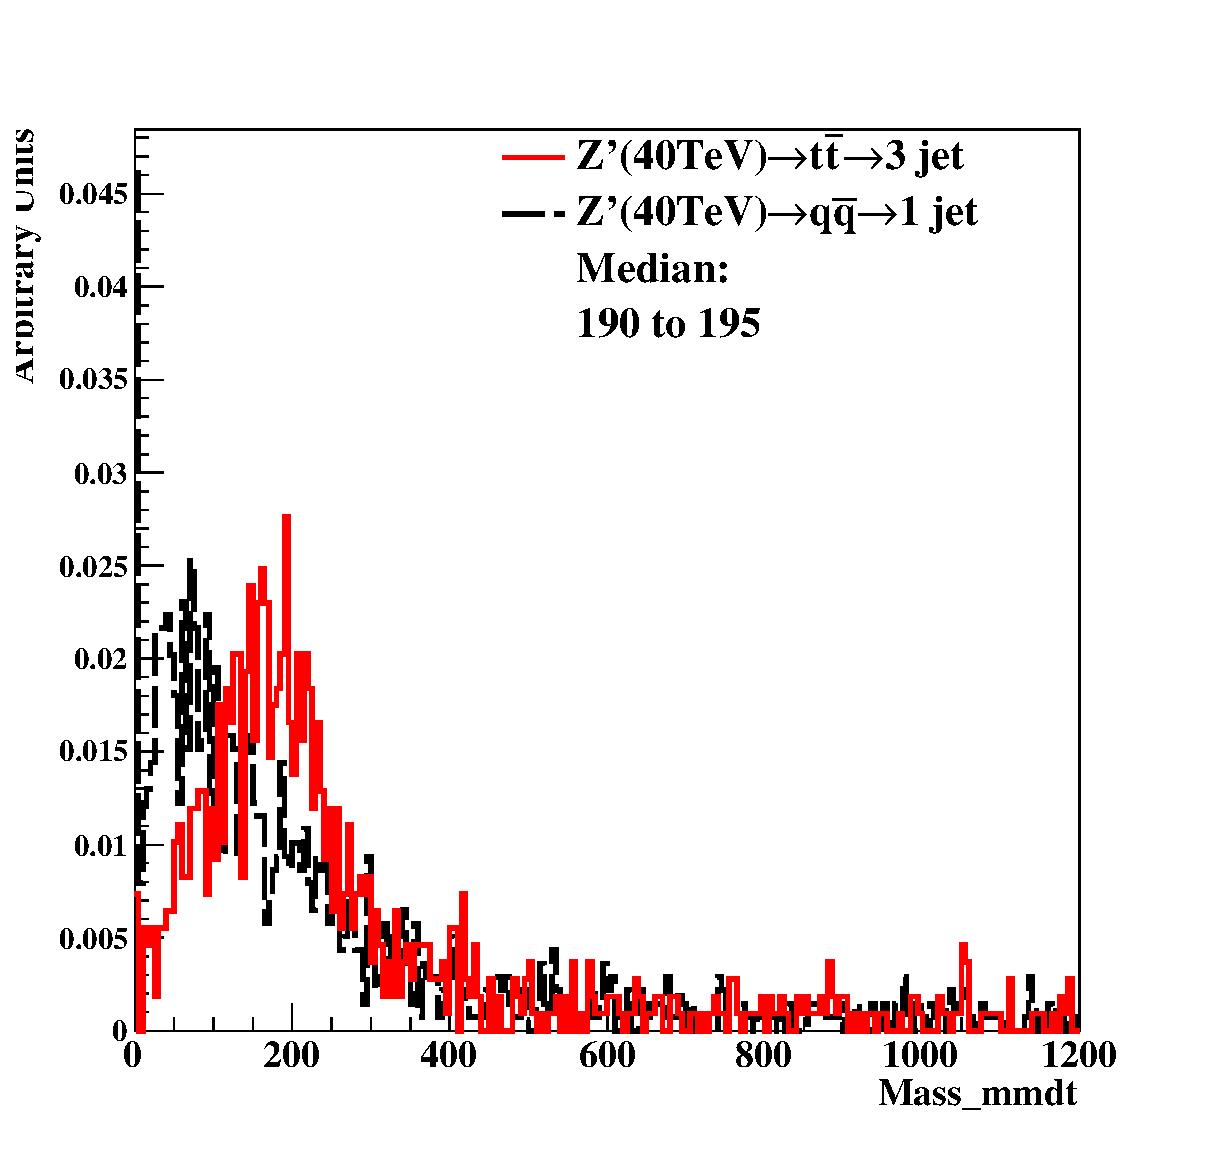
\includegraphics[width=0.43\textwidth]{figs/Dis_cluster_009_mass_mmdt_tt_40tev_04_tt.eps}
   }
   \subfigure[20TeV at 1$\times$1(cm$\times$cm) in cluster] {
   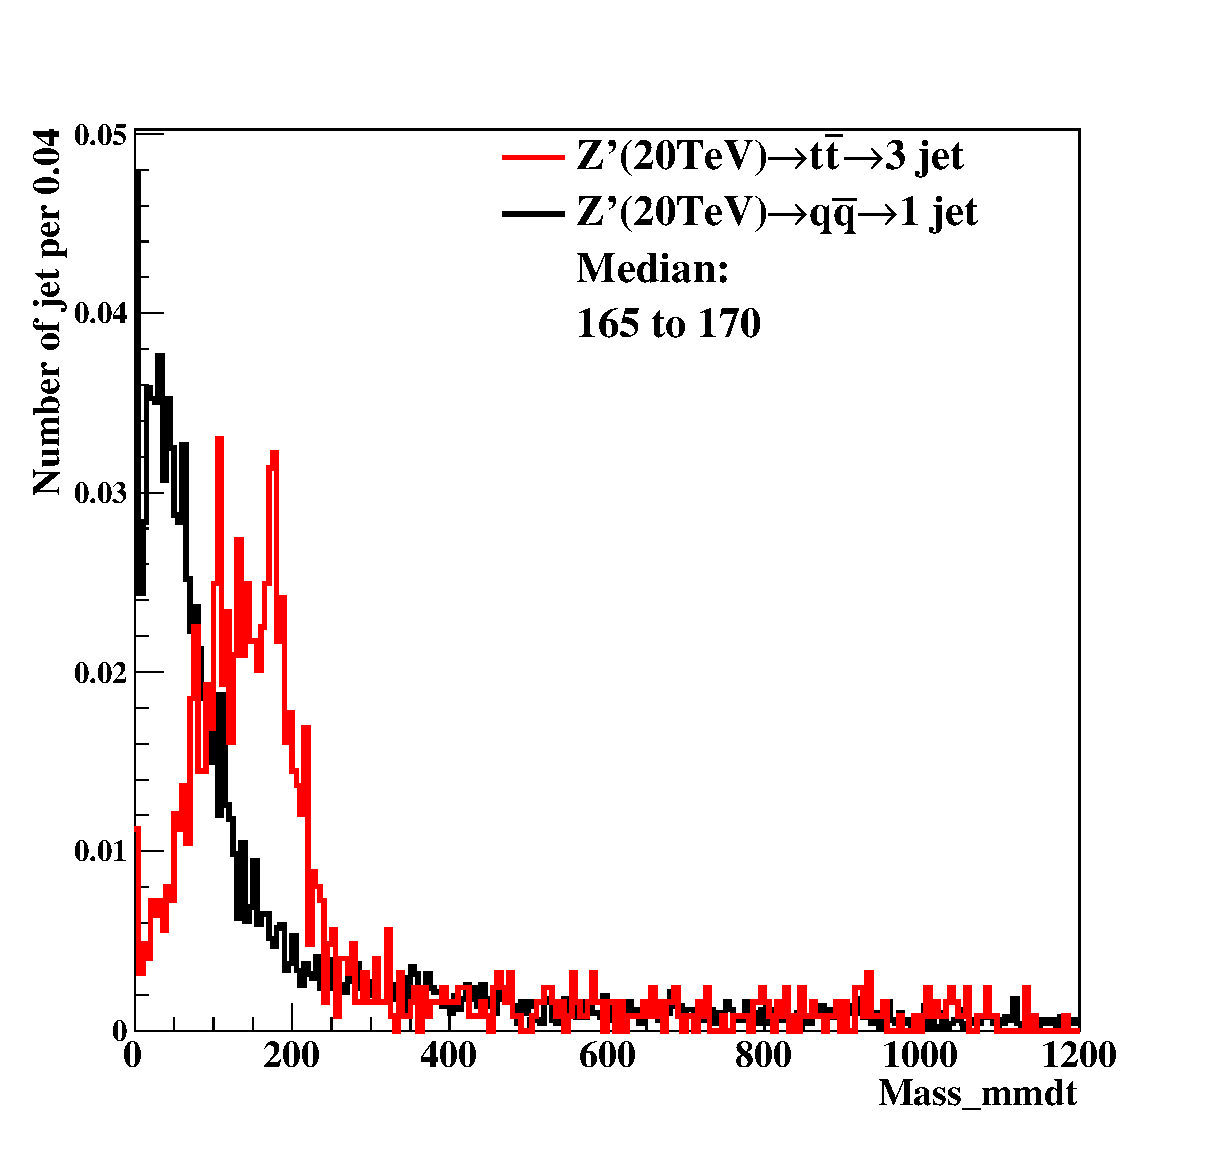
\includegraphics[width=0.43\textwidth]{figs/Dis_cluster_012_mass_mmdt_tt_20tev_04_tt.eps}\hfill
   }
      \subfigure[40TeV at 1$\times$1(cm$\times$cm) in cluster] {
   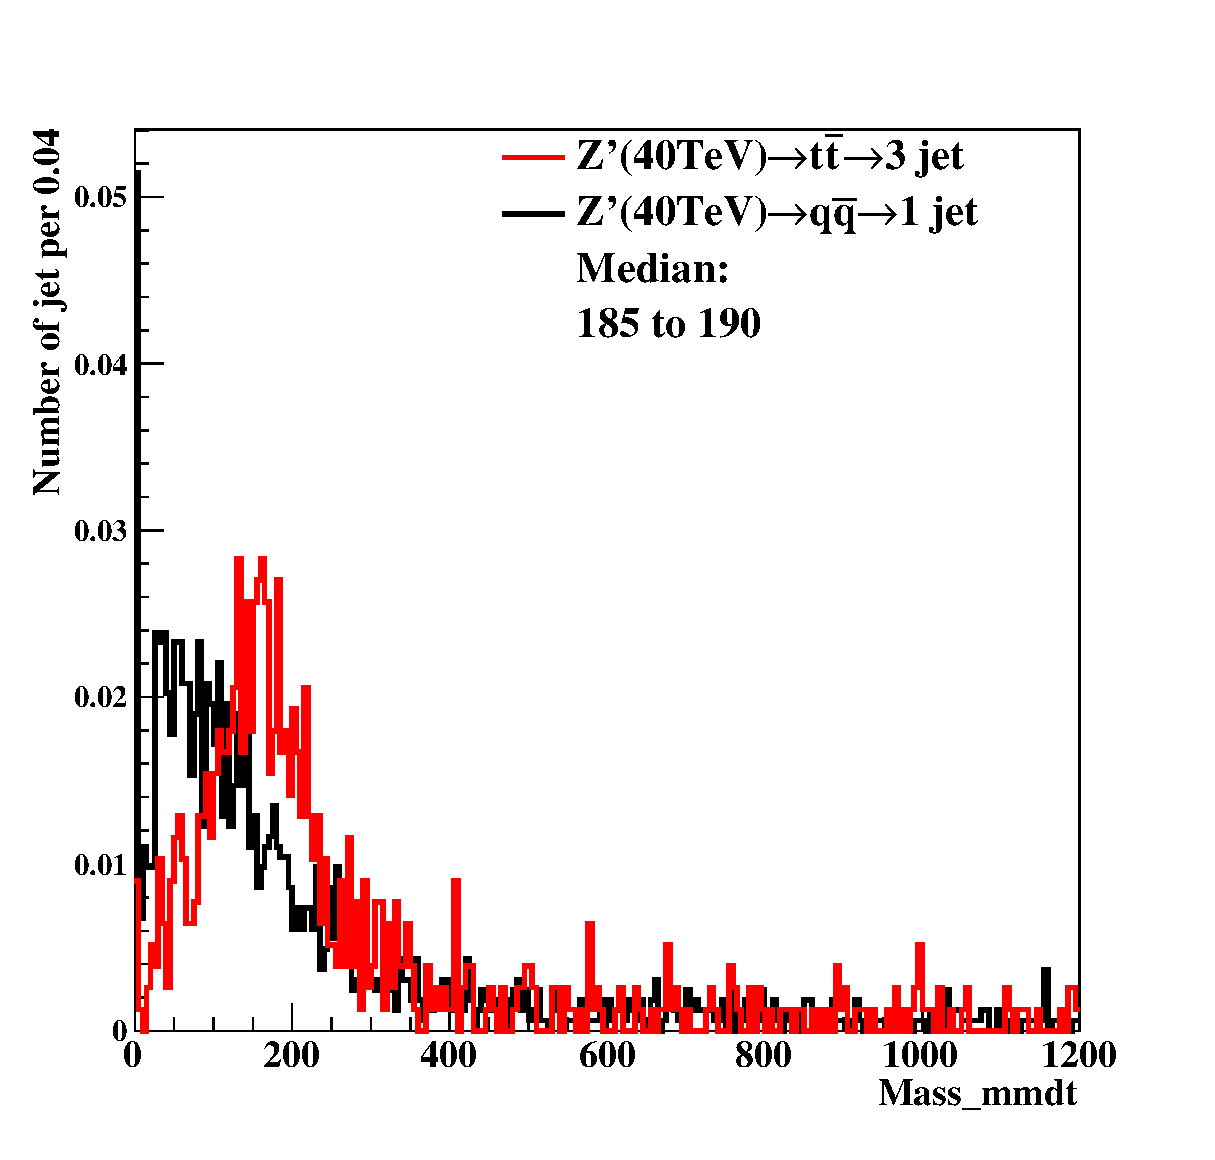
\includegraphics[width=0.43\textwidth]{figs/Dis_cluster_012_mass_mmdt_tt_40tev_04_tt.eps}
   }
\end{center}
\caption{Distributions of mass soft drop at $\beta$=0, signal=tt, in 20,40TeV energy of collision  in different detector sizes. Cell Size in 20$\times$20, 5$\times$5, and 1$\times$1(cm$\times$cm) are shown here.}
\label{fig:cluster_tau21_tau32}
\end{figure}

\begin{figure}
\begin{center}
  \subfigure[Central at Median($20\times20$=150,$5\times5$=150,$1\times1$=150) change width in cluster at 5TeV] {
  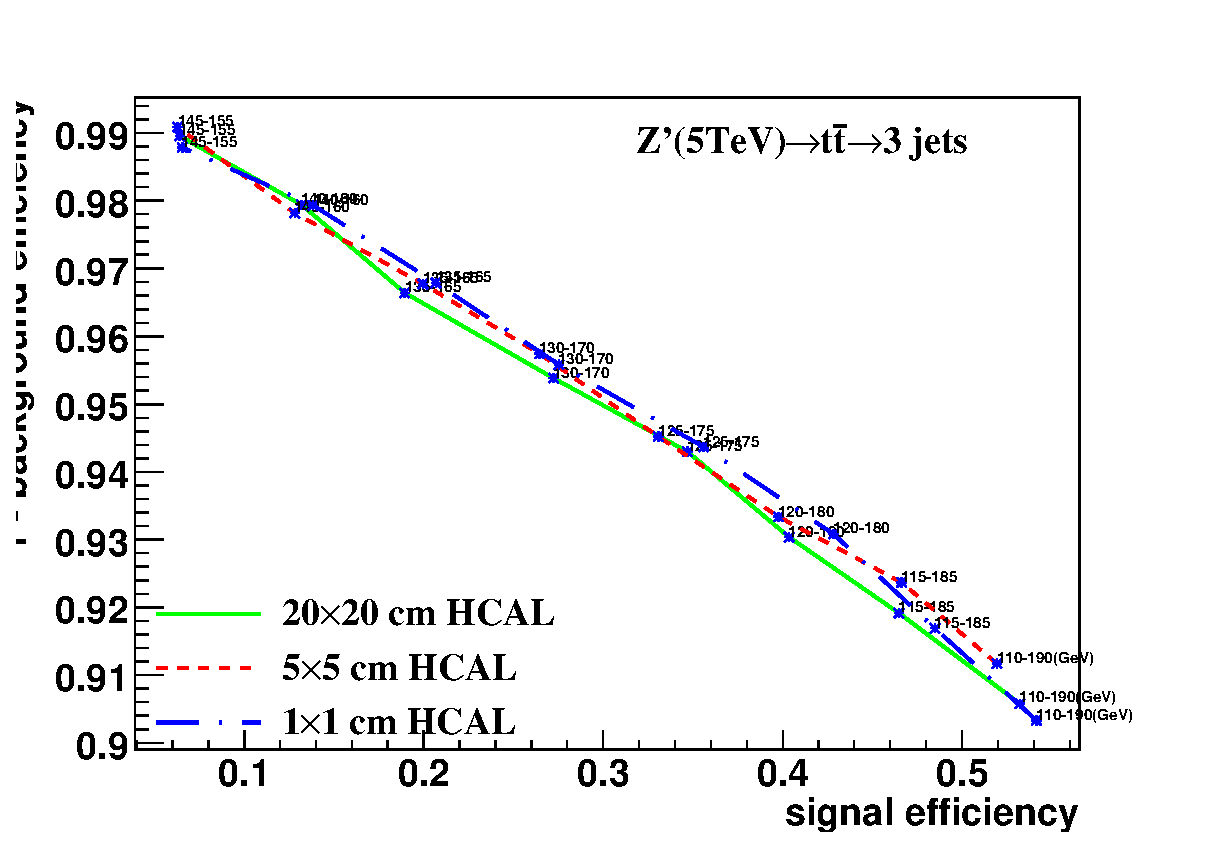
\includegraphics[width=0.43\textwidth]{figs/A_Cluster_mass_mmdt_5tev_eff_1_central_fix_tt_qq.eps}
  }
  \subfigure[Central at Median($20\times20$=155,$5\times5$=150,$1\times1$=155) change width in cluster at 10TeV] {
  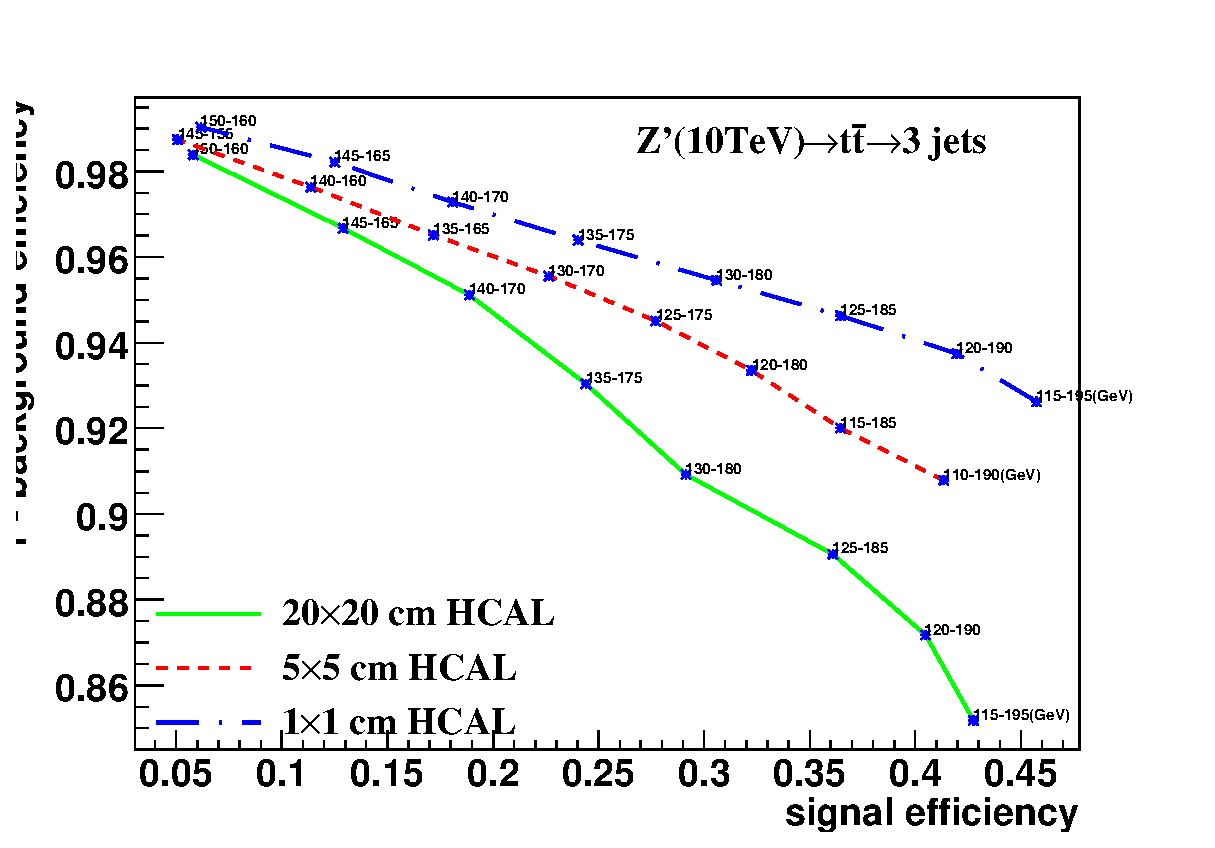
\includegraphics[width=0.43\textwidth]{figs/A_Cluster_mass_mmdt_10tev_eff_1_central_fix_tt_qq.eps}
  }
 \subfigure[Central at Median($20\times20$=165,$5\times5$=175,$1\times1$=170) change width in cluster at 20TeV] {
 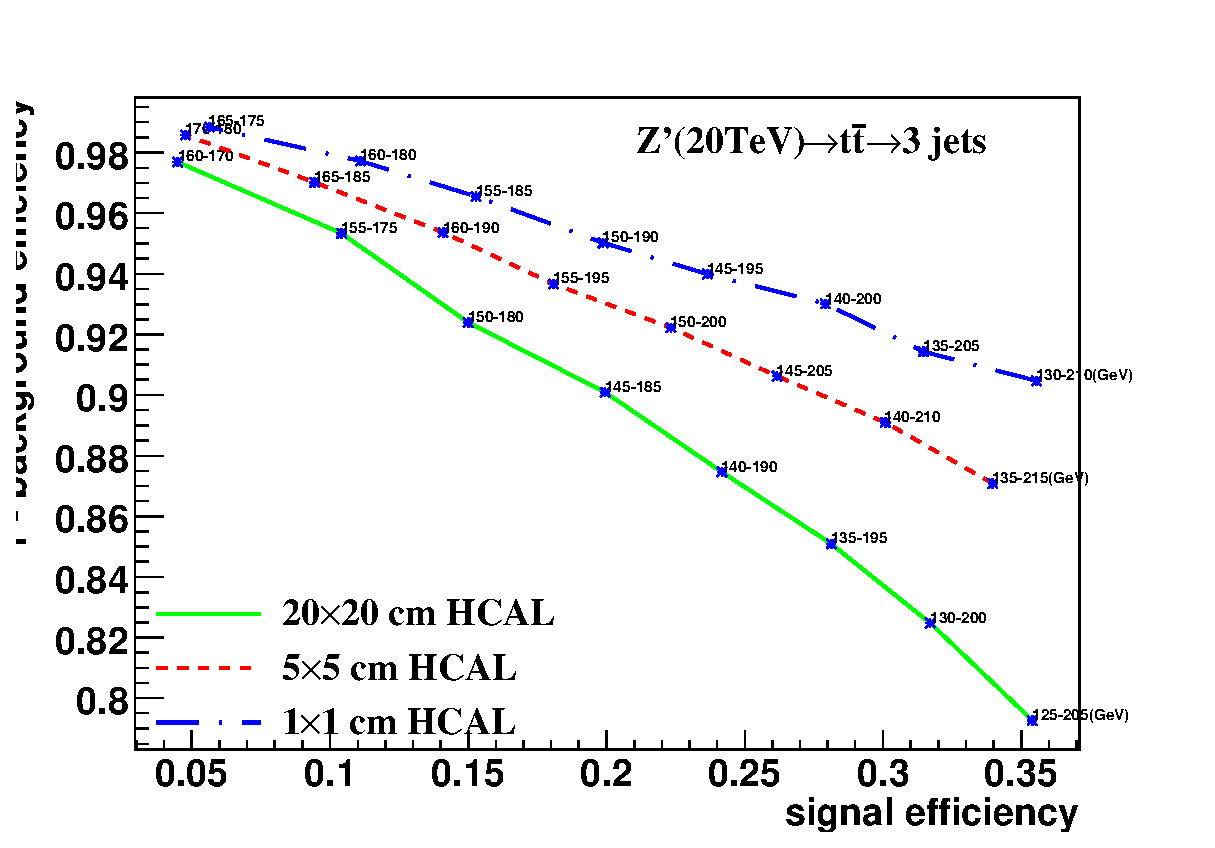
\includegraphics[width=0.43\textwidth]{figs/A_Cluster_mass_mmdt_20tev_eff_1_central_fix_tt_qq.eps}
 }
 \subfigure[Central at Median($20\times20$=190,$5\times5$=200,$1\times1$=190) change width in cluster at 40TeV] {
 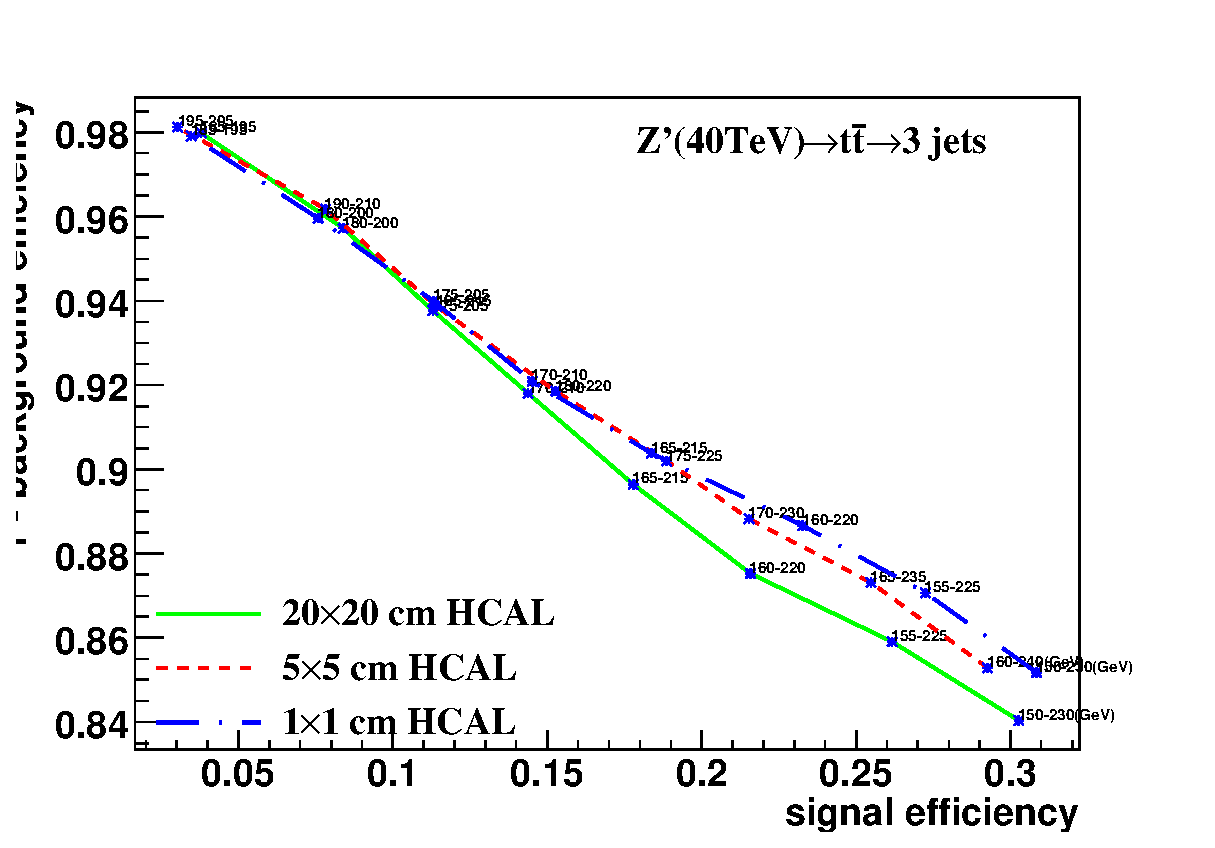
\includegraphics[width=0.43\textwidth]{figs/A_Cluster_mass_mmdt_40tev_eff_1_central_fix_tt_qq.eps}
 }
\end{center}
\caption{study of "fix central and change width" in mass soft drop at $\beta$=0, signal=tt, in 5, 10, 20, 40TeV energy of collision  in different detector sizes. Cell Size in 20$\times$20, 5$\times$5, and 1$\times$1(cm$\times$cm) are shown in each picture.}
\label{fig:cluster_tau21_tau32}
\end{figure}

\begin{figure}
\begin{center}
  \subfigure[Central at Median($20\times20$=150,$5\times5$=150,$1\times1$=150) change width in cluster at 5TeV] {
  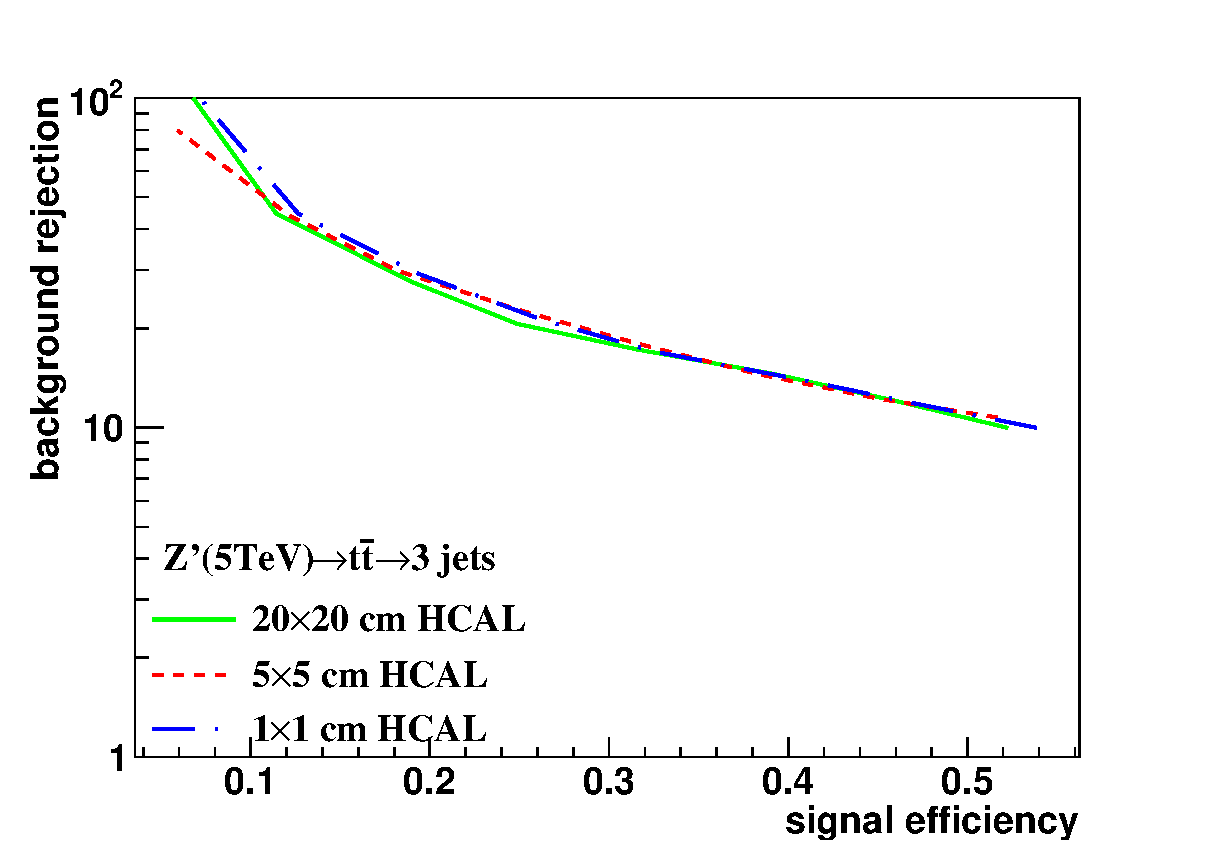
\includegraphics[width=0.43\textwidth]{figs/A_Cluster_mass_mmdt_5tev_eff_1_central_fix_tt_qq_log.eps}
  }
  \subfigure[Central at Median($20\times20$=155,$5\times5$=150,$1\times1$=155) change width in cluster at 10TeV] {
  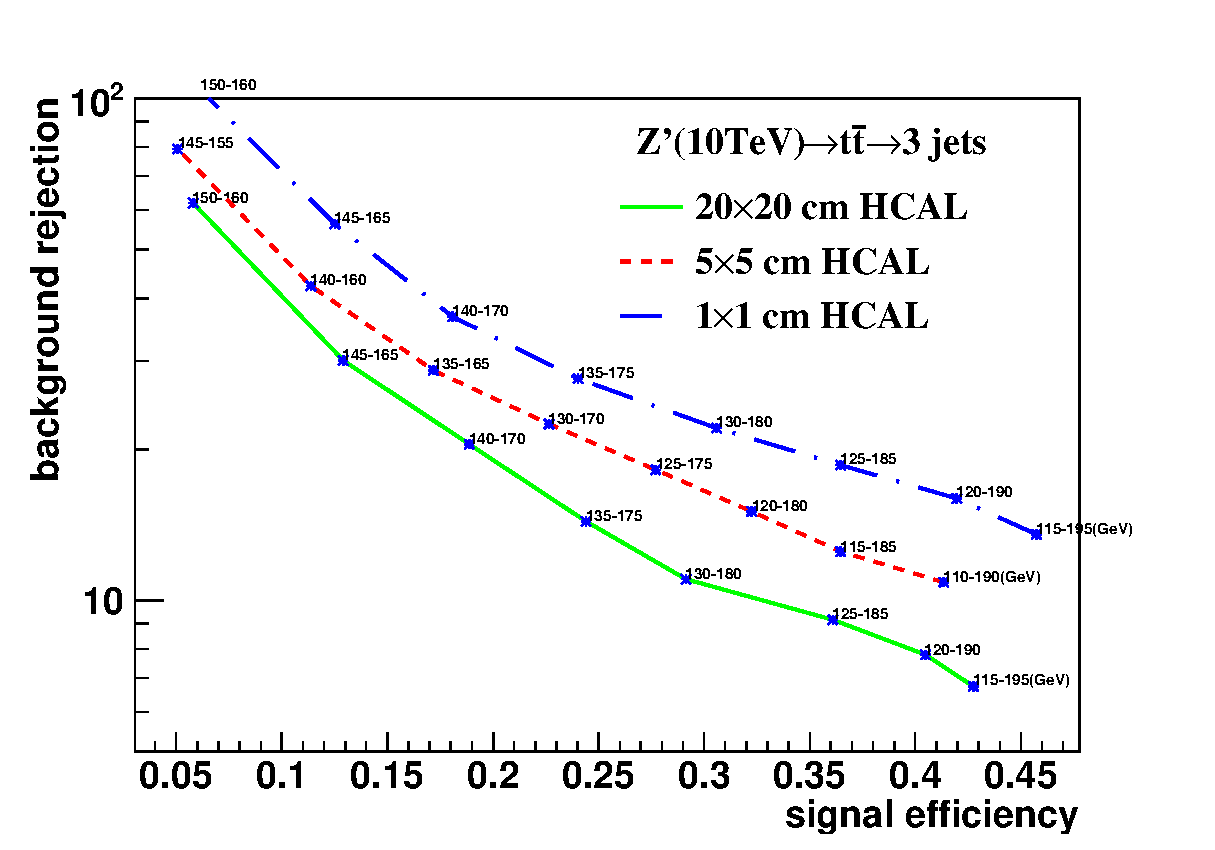
\includegraphics[width=0.43\textwidth]{figs/A_Cluster_mass_mmdt_10tev_eff_1_central_fix_tt_qq_log.eps}
  }
 \subfigure[Central at Median($20\times20$=165,$5\times5$=175,$1\times1$=170) change width in cluster at 20TeV] {
 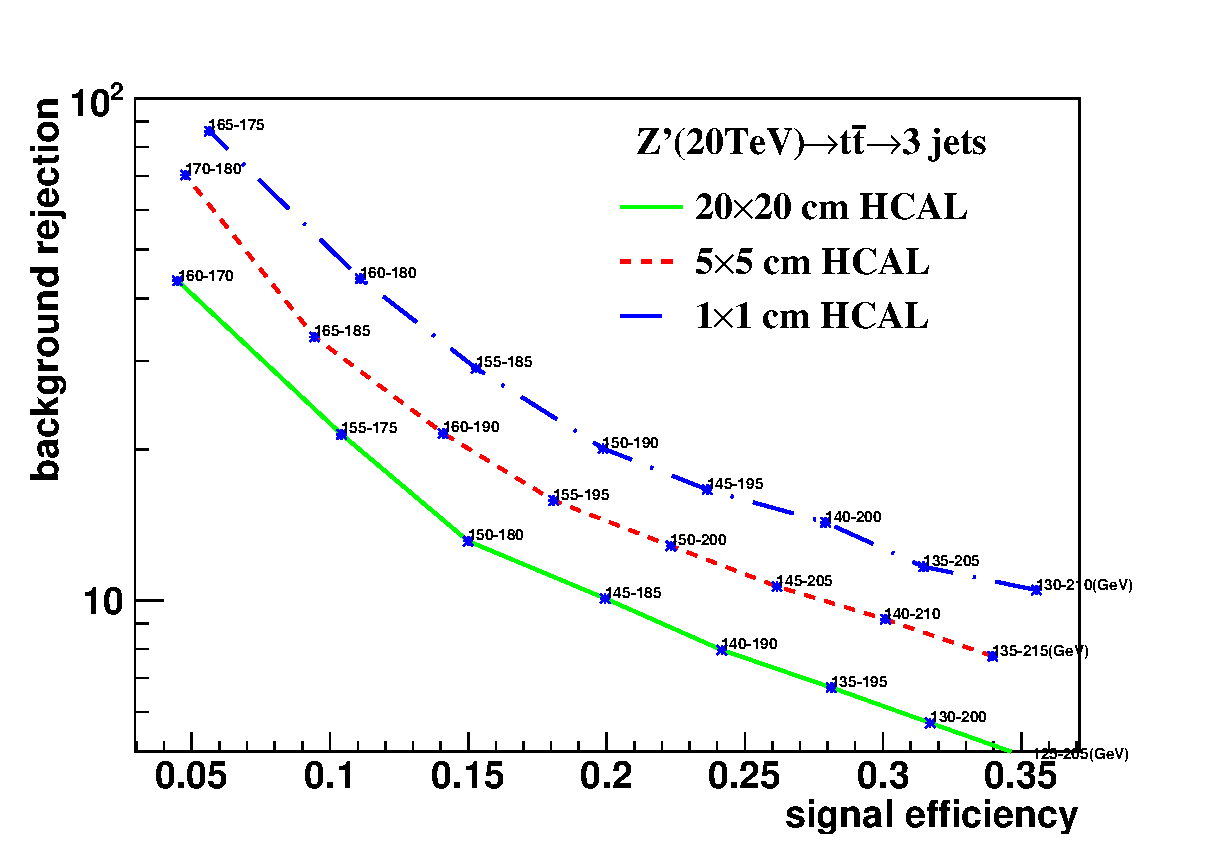
\includegraphics[width=0.43\textwidth]{figs/A_Cluster_mass_mmdt_20tev_eff_1_central_fix_tt_qq_log.eps}
 }
 \subfigure[Central at Median($20\times20$=190,$5\times5$=200,$1\times1$=190) change width in cluster at 40TeV] {
 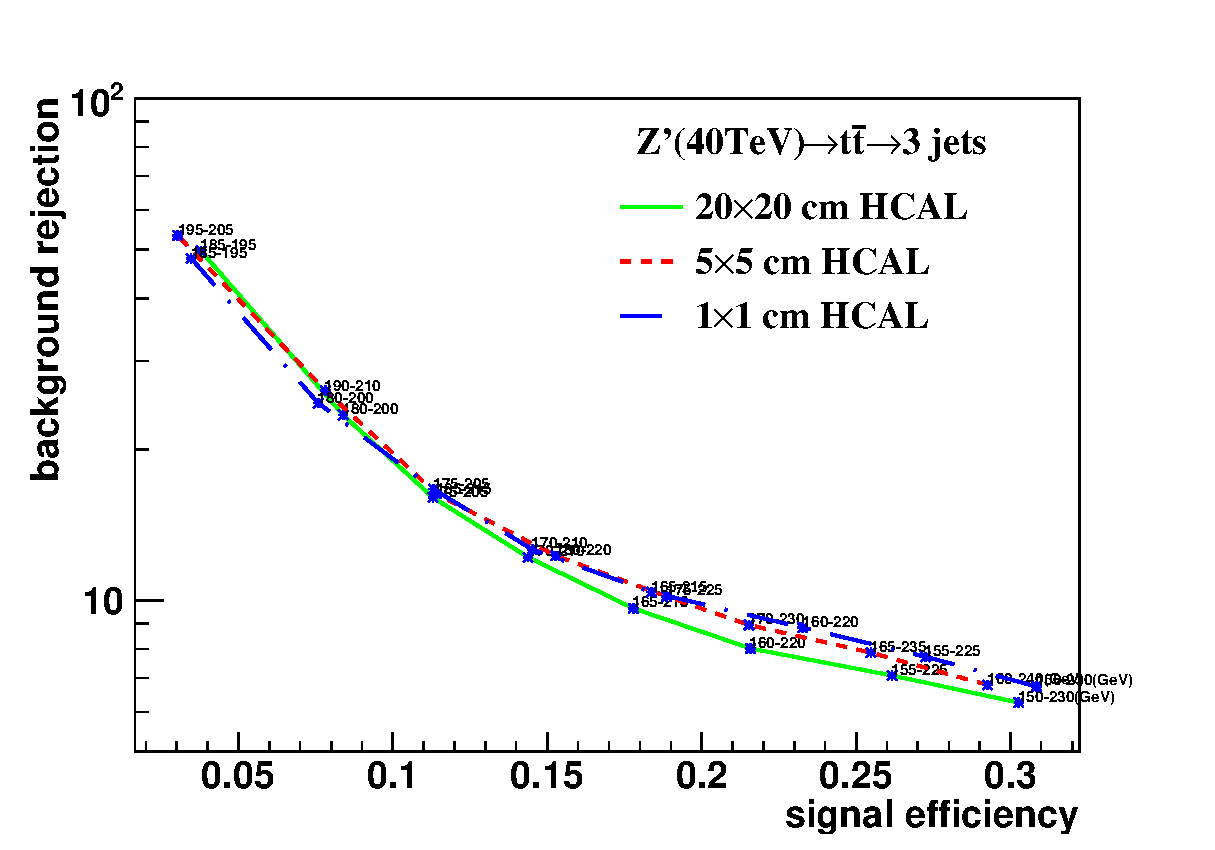
\includegraphics[width=0.43\textwidth]{figs/A_Cluster_mass_mmdt_40tev_eff_1_central_fix_tt_qq_log.eps}
 }
\end{center}
\caption{study of "fix central and change width" in mass soft drop at $\beta$=0, signal=tt, in 5, 10, 20, 40TeV energy of collision  in different detector sizes. Cell Size in 20$\times$20, 5$\times$5, and 1$\times$1(cm$\times$cm) are shown in each picture.}
\label{fig:cluster_tau21_tau32}
\end{figure}


\begin{figure}
\begin{center}
   \subfigure[5TeV at 20$\times$20(cm$\times$cm) in cluster] {
   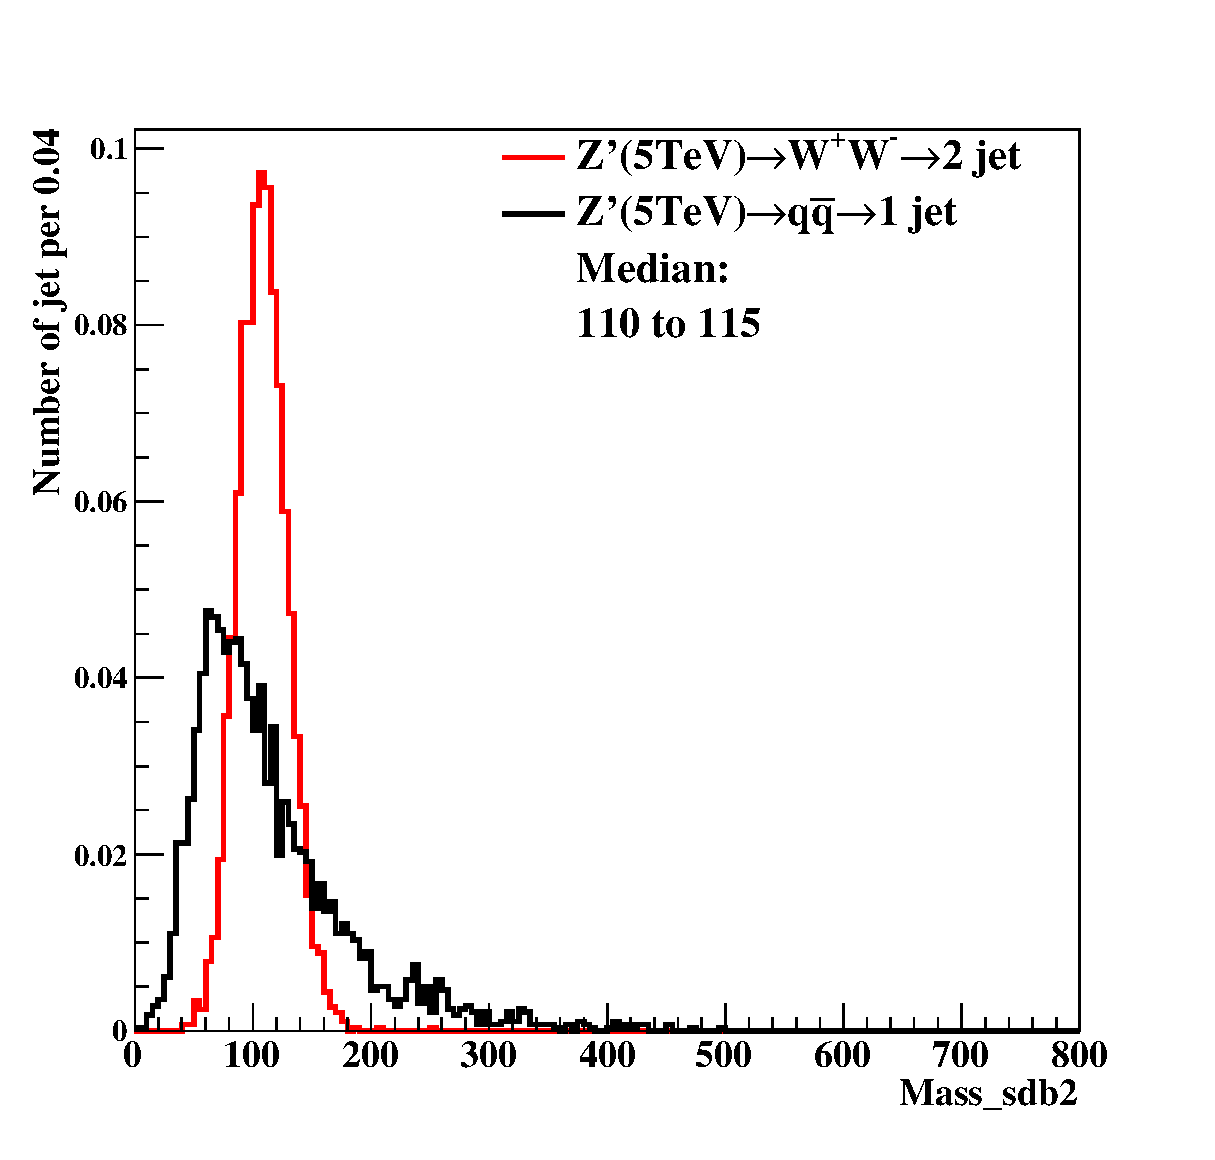
\includegraphics[width=0.43\textwidth]{figs/Dis_cluster_010_mass_sdb2_ww_5tev_04_800.eps}
   }
      \subfigure[10TeV at 20$\times$20(cm$\times$cm) in cluster] {
   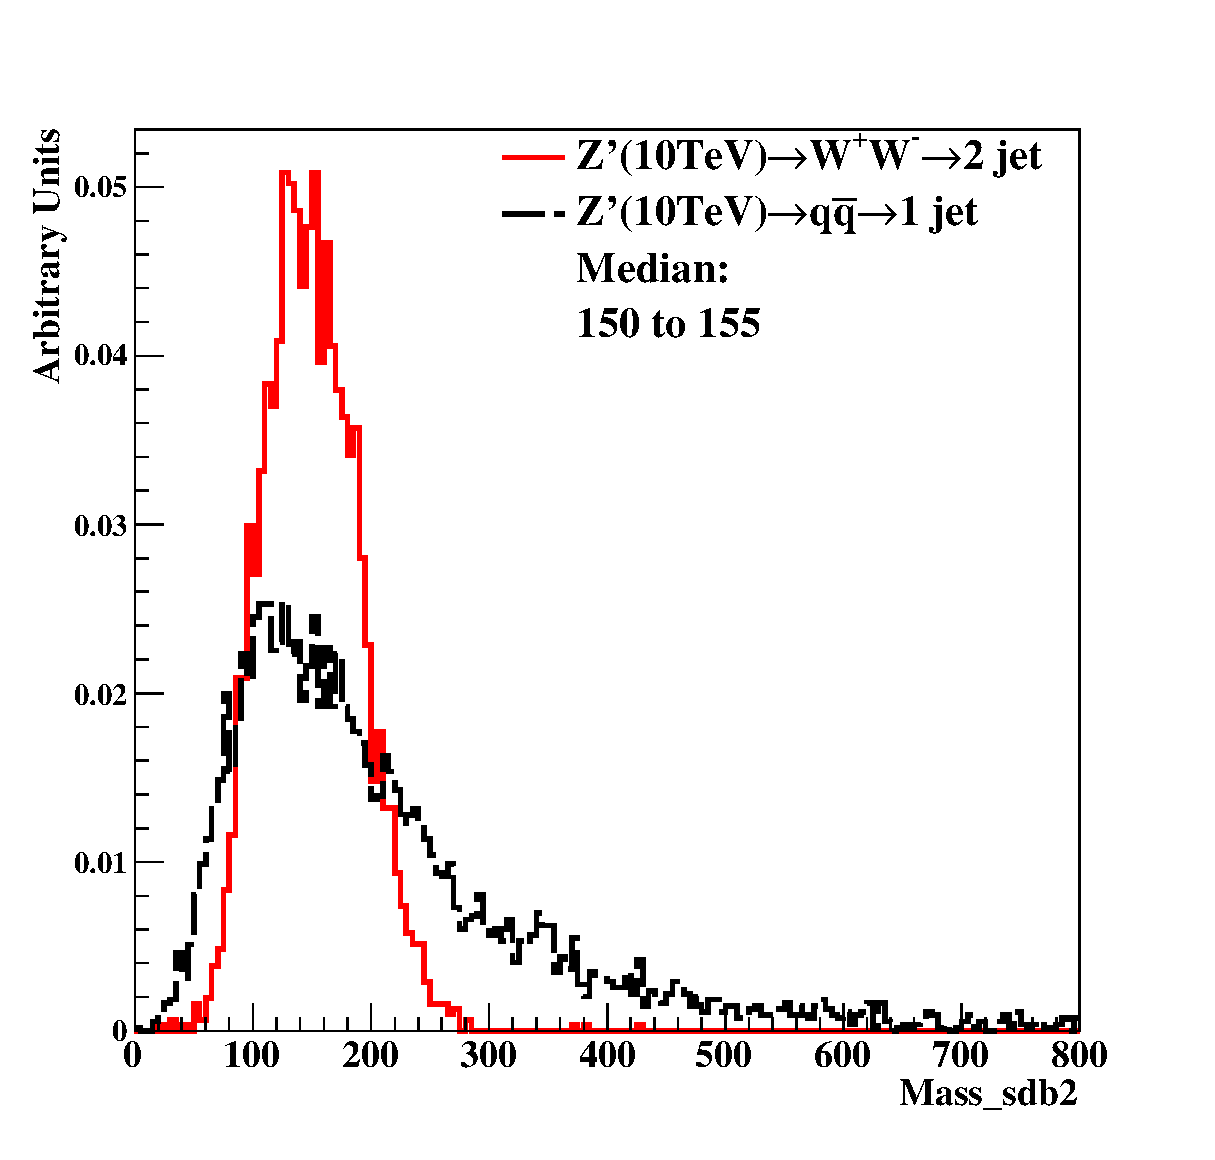
\includegraphics[width=0.43\textwidth]{figs/Dis_cluster_010_mass_sdb2_ww_10tev_04_800.eps}
   }
   \subfigure[5TeV at 5$\times$5(cm$\times$cm) in cluster] {
   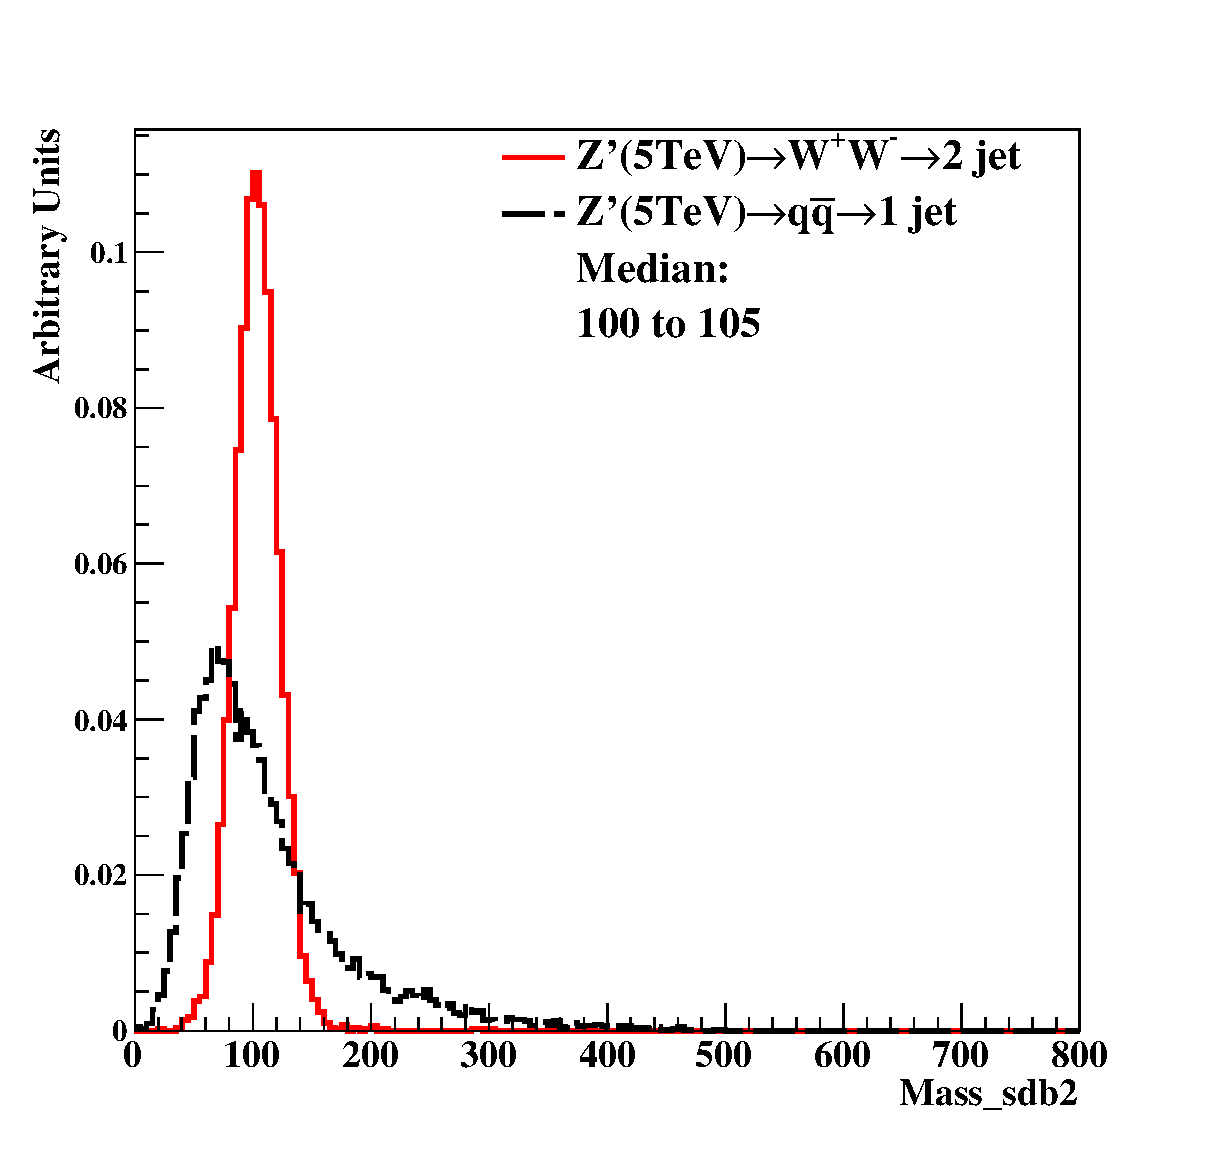
\includegraphics[width=0.43\textwidth]{figs/Dis_cluster_009_mass_sdb2_ww_5tev_04_800.eps}
   }
    \subfigure[10TeV at 5$\times$5(cm$\times$cm) in cluster] {
   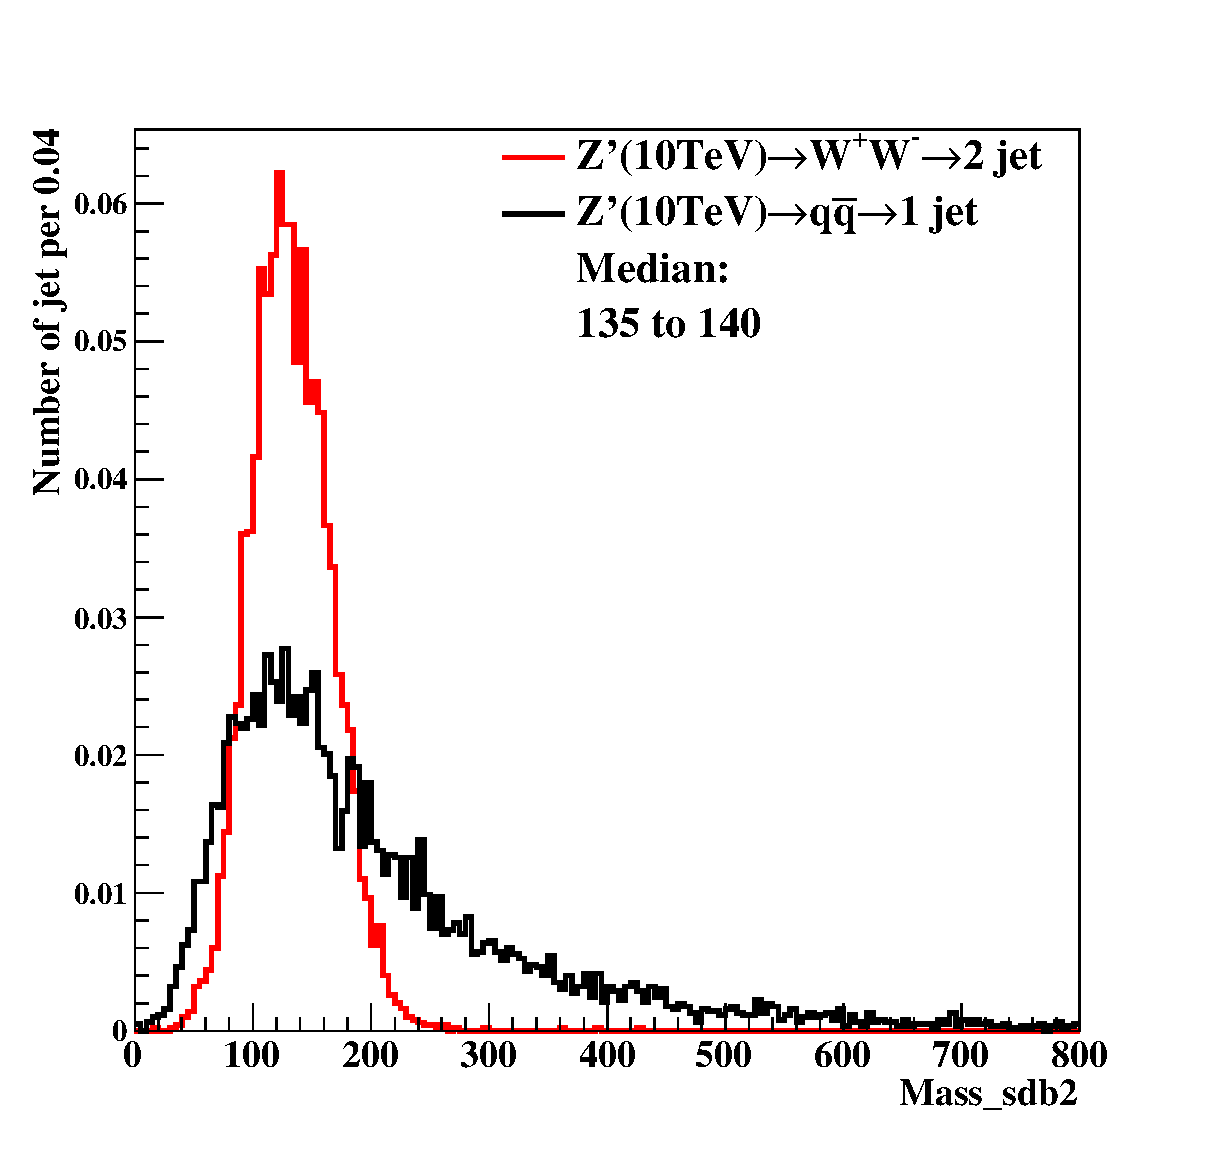
\includegraphics[width=0.43\textwidth]{figs/Dis_cluster_009_mass_sdb2_ww_10tev_04_800.eps}
   }
   \subfigure[5TeV at 1$\times$1(cm$\times$cm) in cluster] {
   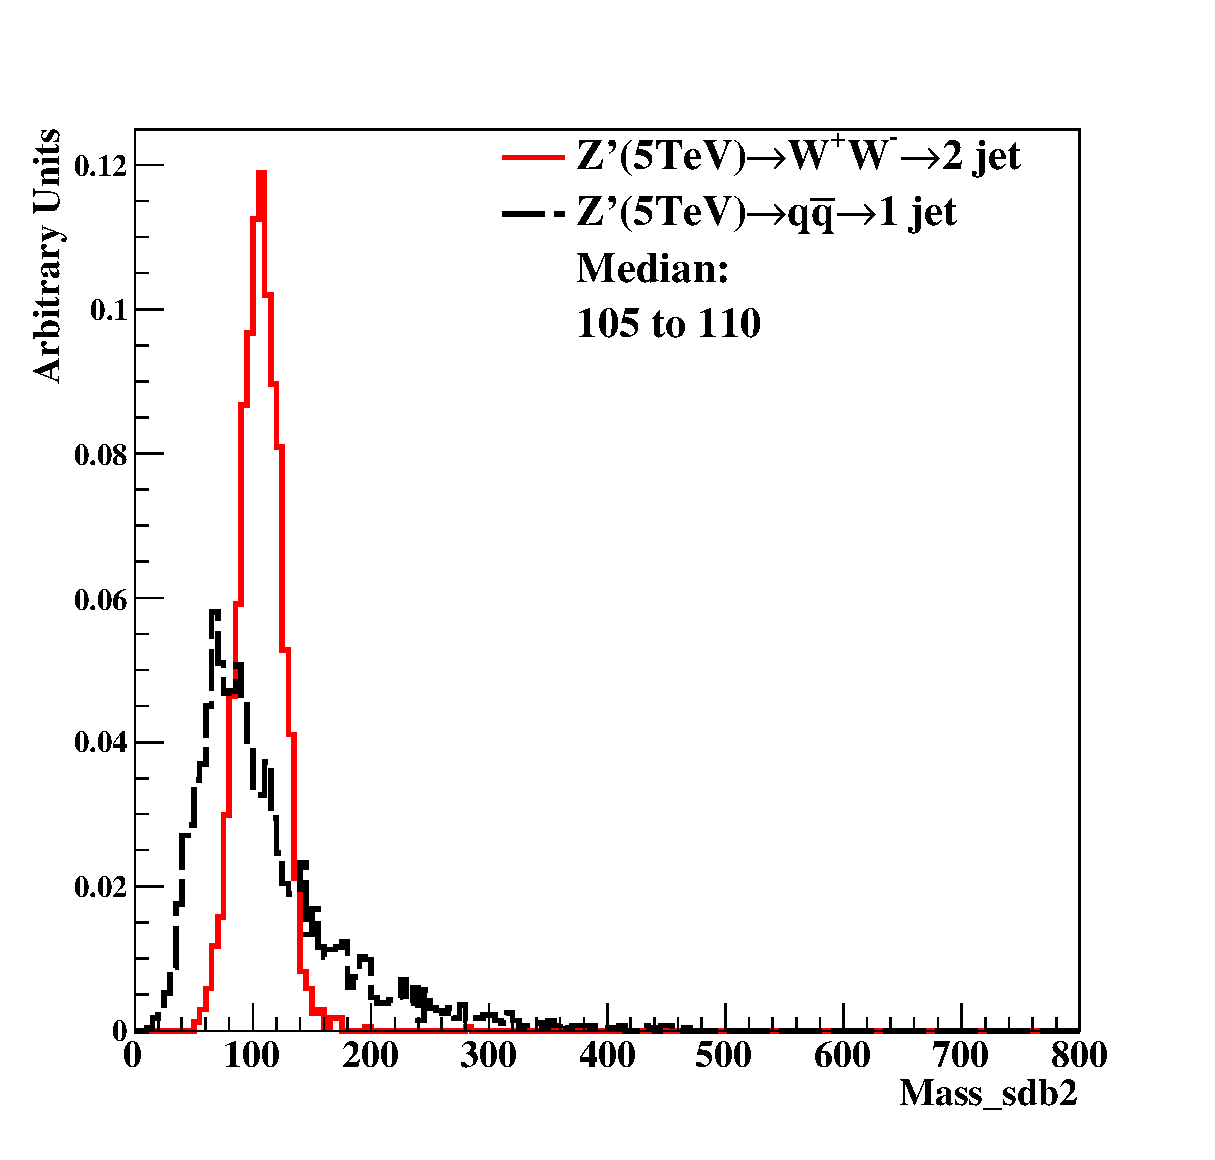
\includegraphics[width=0.43\textwidth]{figs/Dis_cluster_012_mass_sdb2_ww_5tev_04_800.eps}
   }
   \subfigure[10TeV at 1$\times$1(cm$\times$cm) in cluster] {
   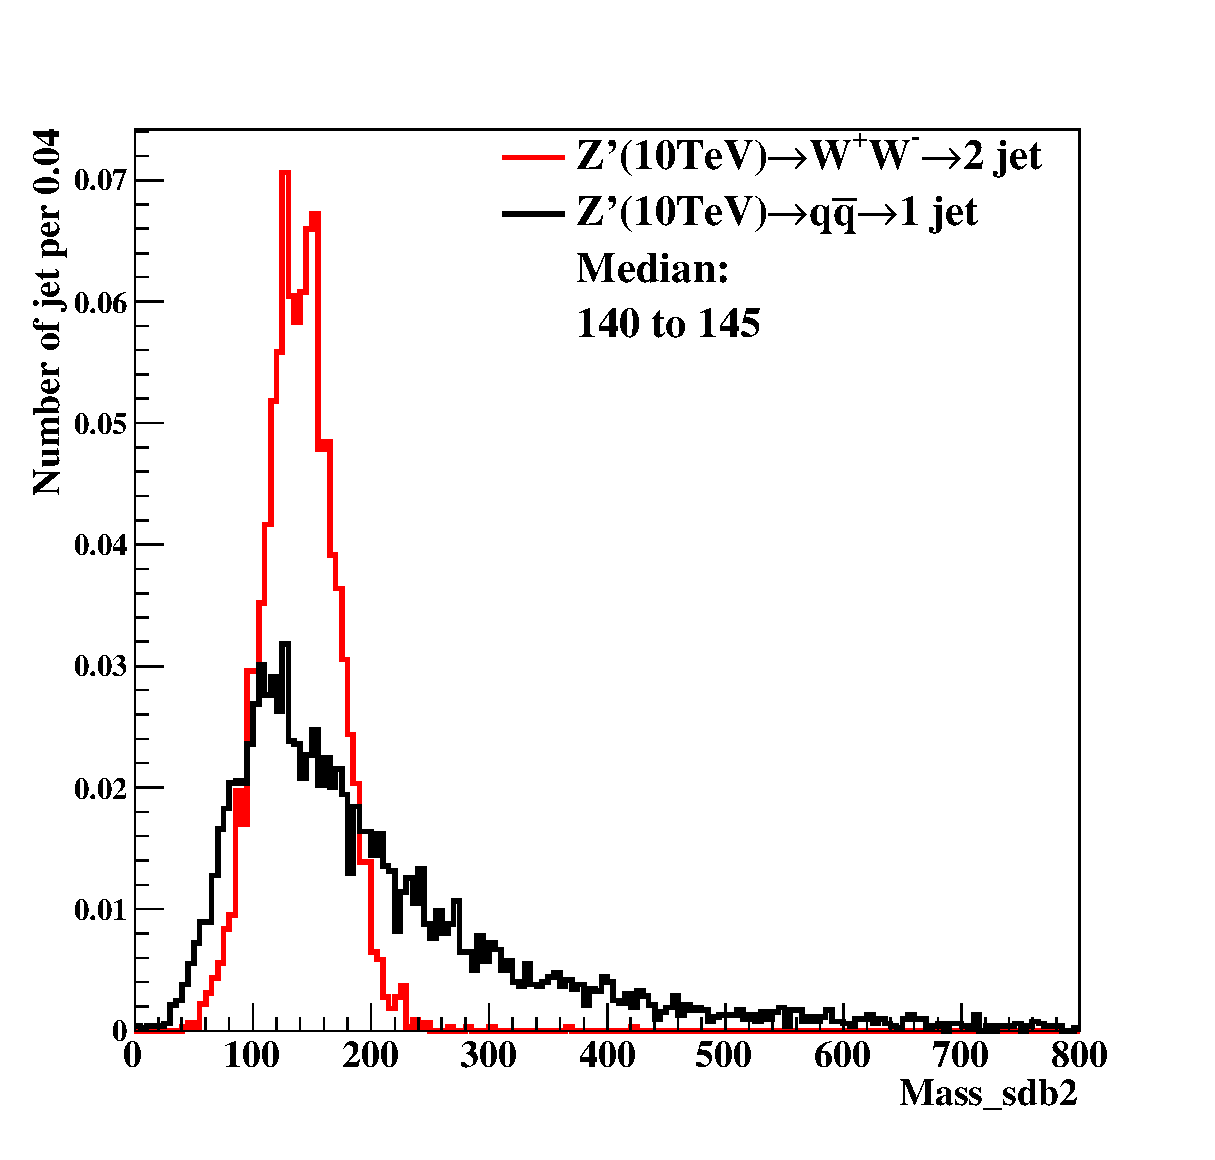
\includegraphics[width=0.43\textwidth]{figs/Dis_cluster_012_mass_sdb2_ww_10tev_04_800.eps}
   }
\end{center}
\caption{Distributions of mass soft drop at $\beta$=2, signal=ww, in 5,10TeV energy of collision  in different detector sizes. Cell Size in 20$\times$20, 5$\times$5, and 1$\times$1(cm$\times$cm) are shown here.}
\label{fig:cluster_tau21_tau32}
\end{figure}

\begin{figure}
\begin{center}
   \subfigure[20TeV at 20$\times$20(cm$\times$cm) in cluster] {
   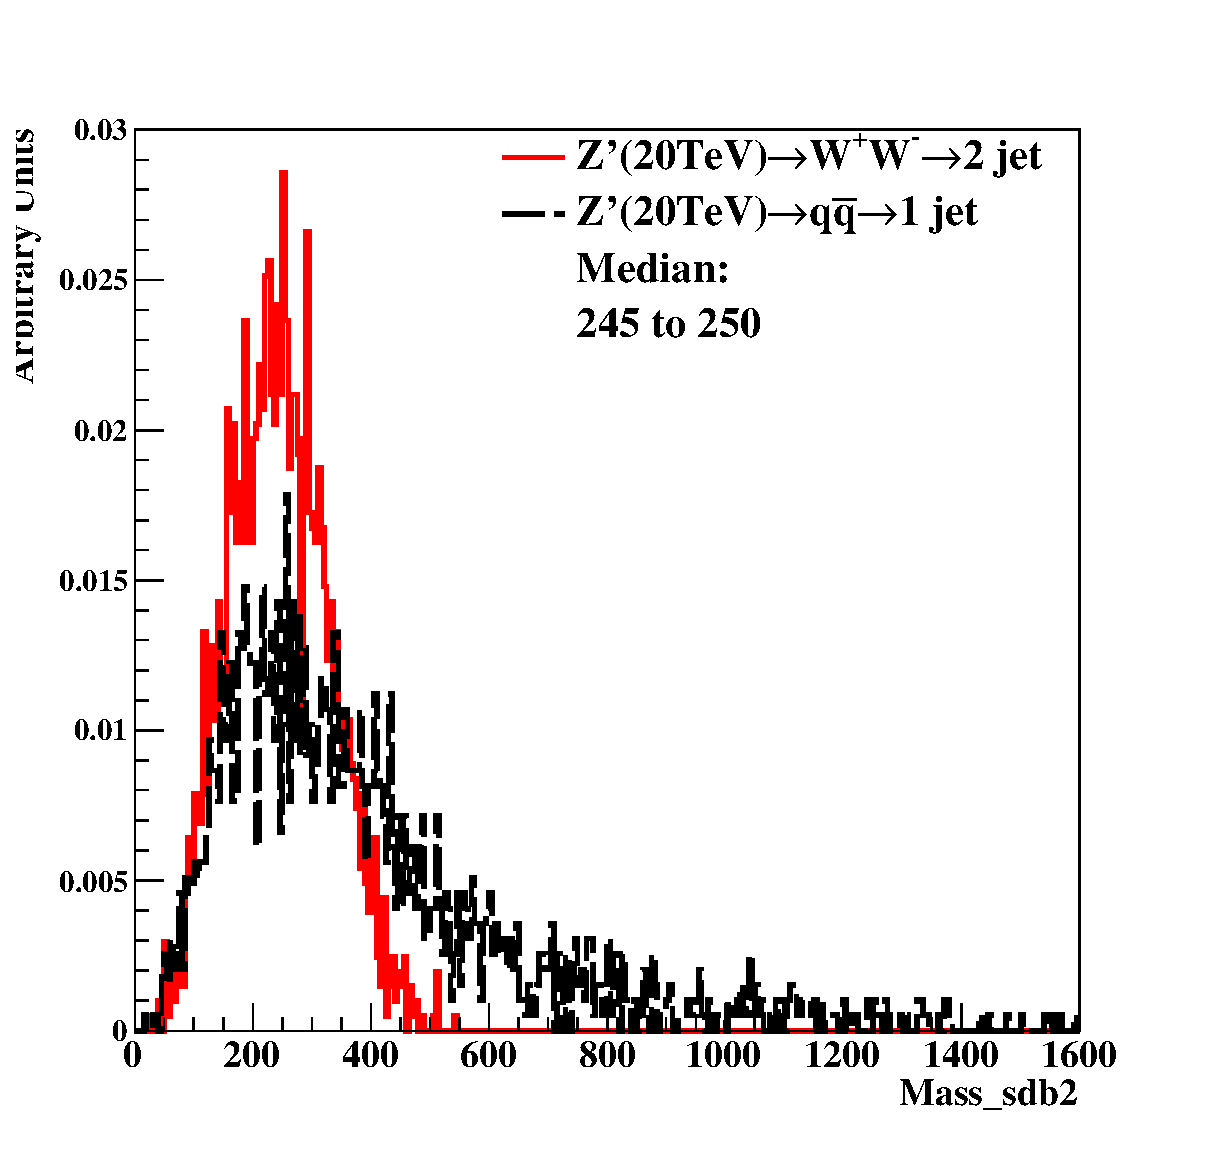
\includegraphics[width=0.43\textwidth]{figs/Dis_cluster_010_mass_sdb2_ww_20tev_04_1600.eps}\hfill
   }
      \subfigure[40TeV at 20$\times$20(cm$\times$cm) in cluster] {
   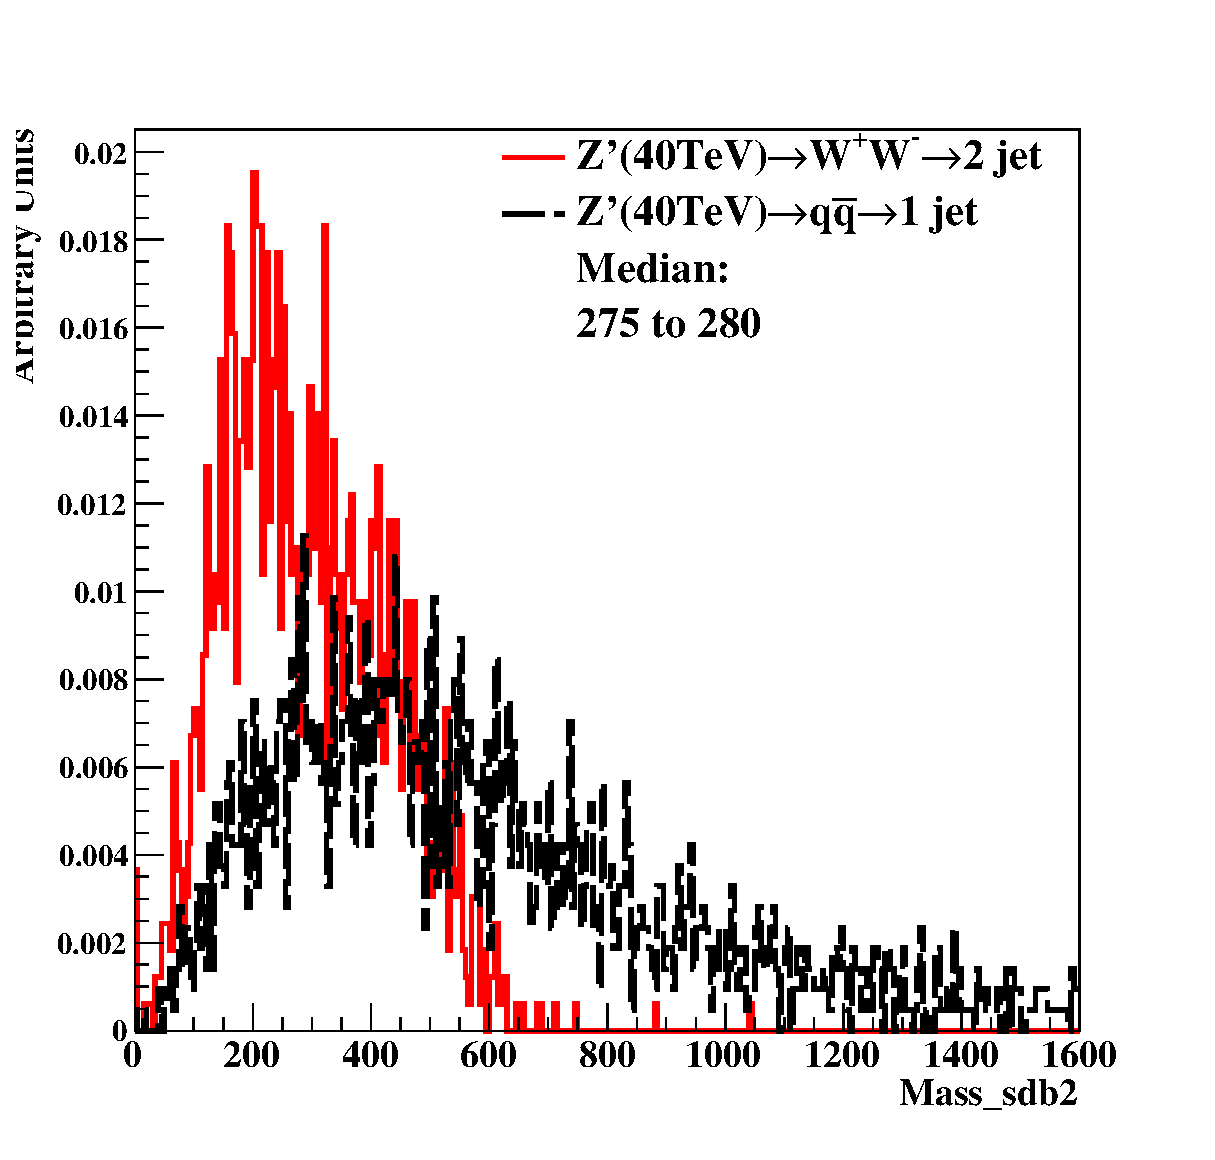
\includegraphics[width=0.43\textwidth]{figs/Dis_cluster_010_mass_sdb2_ww_40tev_04_1600.eps}\hfill
   }
   \subfigure[20TeV at 5$\times$5(cm$\times$cm) in cluster] {
   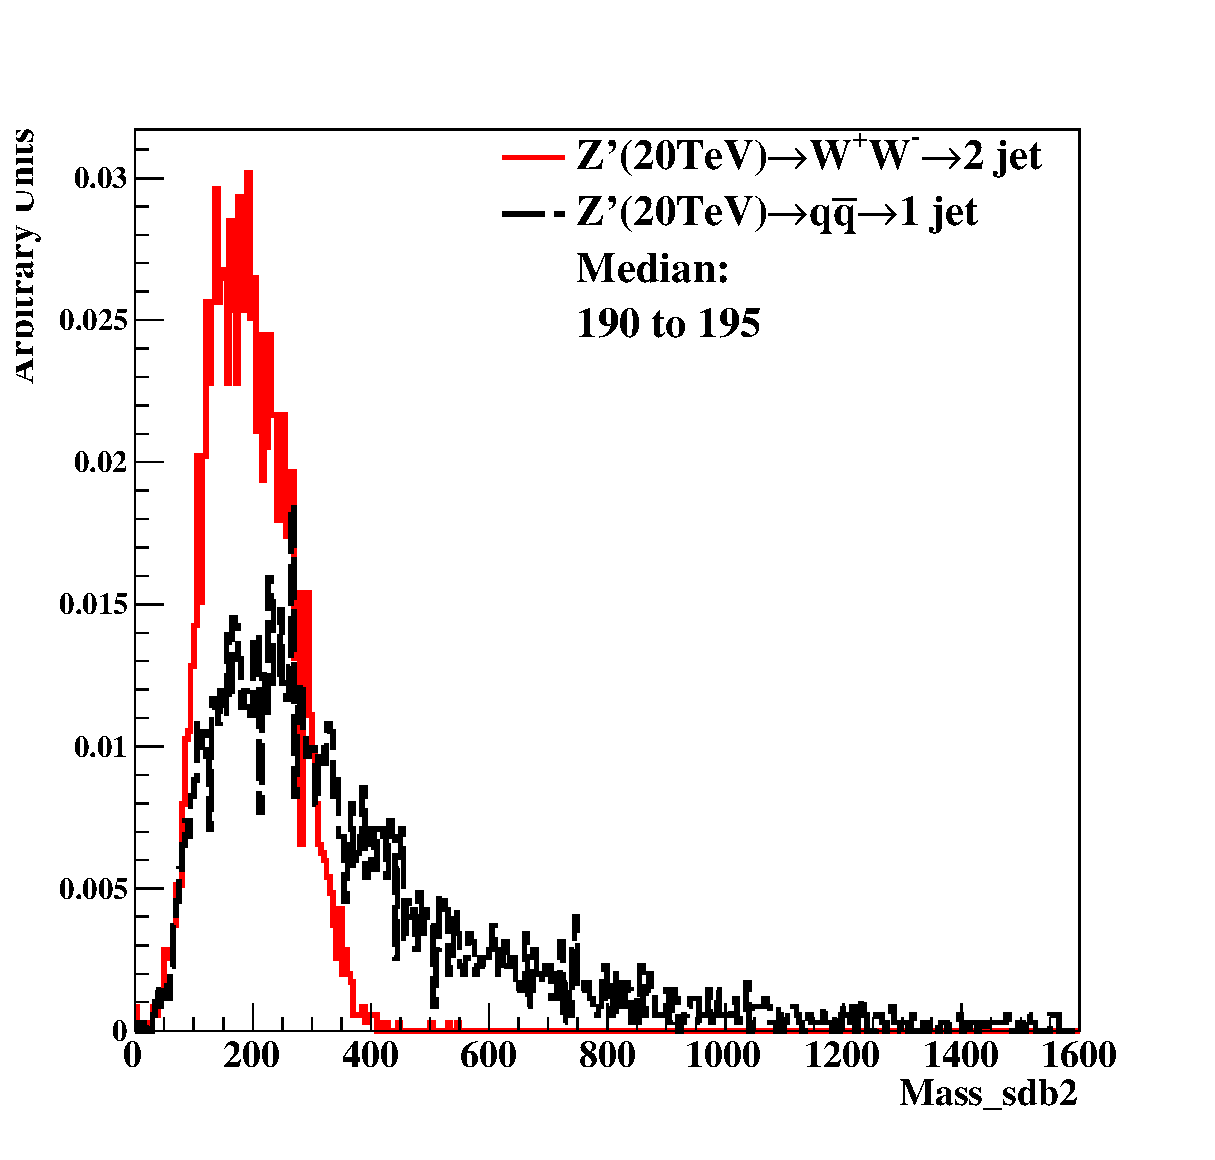
\includegraphics[width=0.43\textwidth]{figs/Dis_cluster_009_mass_sdb2_ww_20tev_04_1600.eps}\hfill
   }
    \subfigure[40TeV at 5$\times$5(cm$\times$cm) in cluster] {
   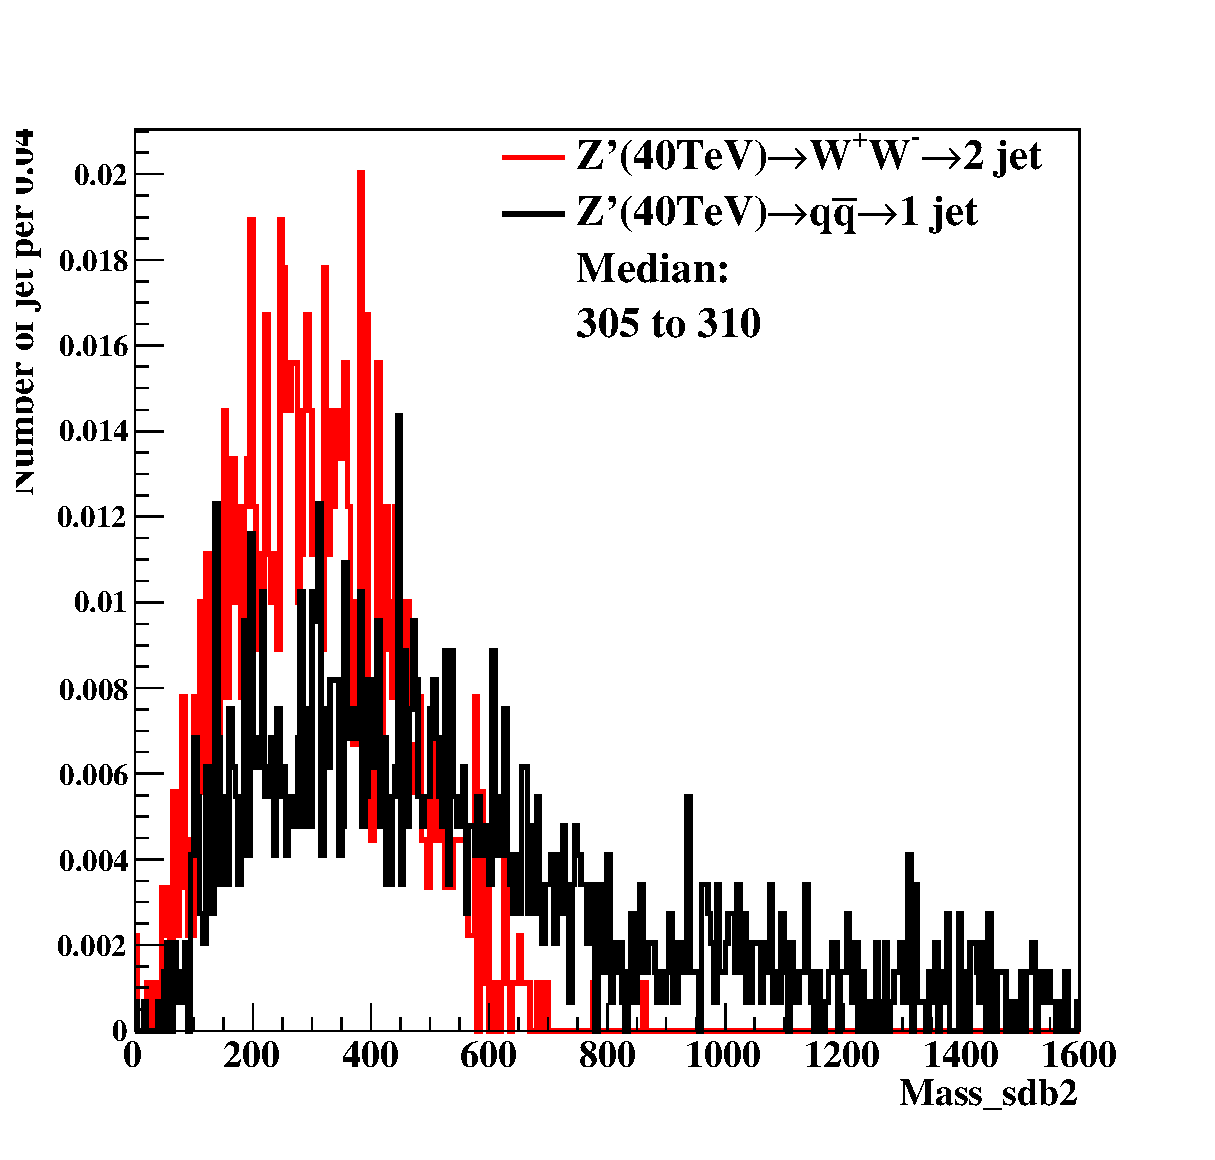
\includegraphics[width=0.43\textwidth]{figs/Dis_cluster_009_mass_sdb2_ww_40tev_04_1600.eps}
   }
   \subfigure[20TeV at 1$\times$1(cm$\times$cm) in cluster] {
   \includegraphics[width=0.43\textwidth]{figs/Dis_cluster_012_mass_sdb2_ww_20tev_04_1600.eps}\hfill
   }
      \subfigure[40TeV at 1$\times$1(cm$\times$cm) in cluster] {
   \includegraphics[width=0.43\textwidth]{figs/Dis_cluster_012_mass_sdb2_ww_40tev_04_1600.eps}
   }
\end{center}
\caption{Distributions of mass soft drop at $\beta$=2, signal=ww, in 20,40TeV energy of collision  in different detector sizes. Cell Size in 20$\times$20, 5$\times$5, and 1$\times$1(cm$\times$cm) are shown here.}
\label{fig:cluster_tau21_tau32}
\end{figure}

\begin{figure}
\begin{center}
  \subfigure[Central at Median($20\times20$=115,$5\times5$=110,$1\times1$=115) change width in cluster at 5TeV] {
  \includegraphics[width=0.43\textwidth]{figs/A_Cluster_mass_sdb2_5tev_eff_1_central_fix_ww_qq.eps}
  }
  \subfigure[Central at Median($20\times20$=155,$5\times5$=140,$1\times1$=145) change width in cluster at 10TeV] {
  \includegraphics[width=0.43\textwidth]{figs/A_Cluster_mass_sdb2_10tev_eff_1_central_fix_ww_qq.eps}
  }
 \subfigure[Central at Median($20\times20$=250,$5\times5$=195,$1\times1$=205) change width in cluster at 20TeV] {
 \includegraphics[width=0.43\textwidth]{figs/A_Cluster_mass_sdb2_20tev_eff_1_central_fix_ww_qq.eps}
 }
 \subfigure[Central at Median($20\times20$=285,$5\times5$=310,$1\times1$=290) change width in cluster at 40TeV] {
 \includegraphics[width=0.43\textwidth]{figs/A_Cluster_mass_sdb2_40tev_eff_1_central_fix_ww_qq.eps}
 }
\end{center}
\caption{study of "fix central and change width" in mass soft drop at $\beta$=2, signal=ww, in 5, 10, 20, 40TeV energy of collision  in different detector sizes. Cell Size in 20$\times$20, 5$\times$5, and 1$\times$1(cm$\times$cm) are shown in each picture.}
\label{fig:cluster_tau21_tau32}
\end{figure}

\begin{figure}
\begin{center}
  \subfigure[Central at Median($20\times20$=115,$5\times5$=110,$1\times1$=115) change width in cluster at 5TeV] {
  \includegraphics[width=0.43\textwidth]{figs/A_Cluster_mass_sdb2_5tev_eff_1_central_fix_ww_qq_log.eps}
  }
  \subfigure[Central at Median($20\times20$=155,$5\times5$=140,$1\times1$=145) change width in cluster at 10TeV] {
  \includegraphics[width=0.43\textwidth]{figs/A_Cluster_mass_sdb2_10tev_eff_1_central_fix_ww_qq_log.eps}
  }
 \subfigure[Central at Median($20\times20$=250,$5\times5$=195,$1\times1$=205) change width in cluster at 20TeV] {
 \includegraphics[width=0.43\textwidth]{figs/A_Cluster_mass_sdb2_20tev_eff_1_central_fix_ww_qq_log.eps}
 }
 \subfigure[Central at Median($20\times20$=285,$5\times5$=310,$1\times1$=290) change width in cluster at 40TeV] {
 \includegraphics[width=0.43\textwidth]{figs/A_Cluster_mass_sdb2_40tev_eff_1_central_fix_ww_qq_log.eps}
 }
\end{center}
\caption{study of "fix central and change width" in mass soft drop at $\beta$=2, signal=ww, in 5, 10, 20, 40TeV energy of collision  in different detector sizes. Cell Size in 20$\times$20, 5$\times$5, and 1$\times$1(cm$\times$cm) are shown in each picture.}
\label{fig:cluster_tau21_tau32}
\end{figure}

\begin{figure}
\begin{center}
   \subfigure[5TeV at 20$\times$20(cm$\times$cm) in cluster] {
   \includegraphics[width=0.43\textwidth]{figs/Dis_cluster_010_mass_sdb2_tt_5tev_04_tt_1200.eps}
   }
      \subfigure[10TeV at 20$\times$20(cm$\times$cm) in cluster] {
   \includegraphics[width=0.43\textwidth]{figs/Dis_cluster_010_mass_sdb2_tt_10tev_04_tt_1200.eps}
   }
   \subfigure[5TeV at 5$\times$5(cm$\times$cm) in cluster] {
   \includegraphics[width=0.43\textwidth]{figs/Dis_cluster_009_mass_sdb2_tt_5tev_04_tt_1200.eps}
   }
    \subfigure[10TeV at 5$\times$5(cm$\times$cm) in cluster] {
   \includegraphics[width=0.43\textwidth]{figs/Dis_cluster_009_mass_sdb2_tt_10tev_04_tt_1200.eps}
   }
   \subfigure[5TeV at 1$\times$1(cm$\times$cm) in cluster] {
   \includegraphics[width=0.43\textwidth]{figs/Dis_cluster_012_mass_sdb2_tt_5tev_04_tt_1200.eps}
   }
   \subfigure[10TeV at 1$\times$1(cm$\times$cm) in cluster] {
   \includegraphics[width=0.43\textwidth]{figs/Dis_cluster_012_mass_sdb2_tt_10tev_04_tt_1200.eps}
   }
\end{center}
\caption{Distributions of mass soft drop at $\beta$=2, signal=tt, in 5,10TeV energy of collision  in different detector sizes. Cell Size in 20$\times$20, 5$\times$5, and 1$\times$1(cm$\times$cm) are shown here.}
\label{fig:cluster_tau21_tau32}
\end{figure}

\begin{figure}
\begin{center}
   \subfigure[20TeV at 20$\times$20(cm$\times$cm) in cluster] {
   \includegraphics[width=0.43\textwidth]{figs/Dis_cluster_010_mass_sdb2_tt_20tev_04_tt_2400.eps}\hfill
   }
      \subfigure[40TeV at 20$\times$20(cm$\times$cm) in cluster] {
   \includegraphics[width=0.43\textwidth]{figs/Dis_cluster_010_mass_sdb2_tt_40tev_04_tt_2400.eps}\hfill
   }
   \subfigure[20TeV at 5$\times$5(cm$\times$cm) in cluster] {
   \includegraphics[width=0.43\textwidth]{figs/Dis_cluster_009_mass_sdb2_tt_20tev_04_tt_2400.eps}\hfill
   }
    \subfigure[40TeV at 5$\times$5(cm$\times$cm) in cluster] {
   \includegraphics[width=0.43\textwidth]{figs/Dis_cluster_009_mass_sdb2_tt_40tev_04_tt_2400.eps}
   }
   \subfigure[20TeV at 1$\times$1(cm$\times$cm) in cluster] {
   \includegraphics[width=0.43\textwidth]{figs/Dis_cluster_012_mass_sdb2_tt_20tev_04_tt_2400.eps}\hfill
   }
      \subfigure[40TeV at 1$\times$1(cm$\times$cm) in cluster] {
   \includegraphics[width=0.43\textwidth]{figs/Dis_cluster_012_mass_sdb2_tt_40tev_04_tt_2400.eps}
   }
\end{center}
\caption{Distributions of mass soft drop at $\beta$=2, signal=tt, in 20,40TeV energy of collision  in different detector sizes. Cell Size in 20$\times$20, 5$\times$5, and 1$\times$1(cm$\times$cm) are shown here.}
\label{fig:cluster_tau21_tau32}
\end{figure}

\begin{figure}
\begin{center}
  \subfigure[Central at Median($20\times20$=185,$5\times5$=185,$1\times1$=185) change width in cluster at 5TeV] {
  \includegraphics[width=0.43\textwidth]{figs/A_Cluster_mass_sdb2_5tev_eff_1_central_fix_tt_qq.eps}
  }
  \subfigure[Central at Median($20\times20$=240,$5\times5$=240,$1\times1$=240) change width in cluster at 10TeV] {
  \includegraphics[width=0.43\textwidth]{figs/A_Cluster_mass_sdb2_10tev_eff_1_central_fix_tt_qq.eps}
  }
 \subfigure[Central at Median($20\times20$=360,$5\times5$=375,$1\times1$=365) change width in cluster at 20TeV] {
 \includegraphics[width=0.43\textwidth]{figs/A_Cluster_mass_sdb2_20tev_eff_1_central_fix_tt_qq.eps}
 }
 \subfigure[Central at Median($20\times20$=620,$5\times5$=625,$1\times1$=630) change width in cluster at 40TeV] {
 \includegraphics[width=0.43\textwidth]{figs/A_Cluster_mass_sdb2_40tev_eff_1_central_fix_tt_qq.eps}
 }
\end{center}
\caption{study of "fix central and change width" in mass soft drop at $\beta$=2, signal=tt, in 5, 10, 20, 40TeV energy of collision  in different detector sizes. Cell Size in 20$\times$20, 5$\times$5, and 1$\times$1(cm$\times$cm) are shown in each picture.}
\label{fig:cluster_tau21_tau32}
\end{figure}

\begin{figure}
\begin{center}
  \subfigure[Central at Median($20\times20$=185,$5\times5$=185,$1\times1$=185) change width in cluster at 5TeV] {
  \includegraphics[width=0.43\textwidth]{figs/A_Cluster_mass_sdb2_5tev_eff_1_central_fix_tt_qq_log.eps}
  }
  \subfigure[Central at Median($20\times20$=240,$5\times5$=240,$1\times1$=240) change width in cluster at 10TeV] {
  \includegraphics[width=0.43\textwidth]{figs/A_Cluster_mass_sdb2_10tev_eff_1_central_fix_tt_qq_log.eps}
  }
 \subfigure[Central at Median($20\times20$=360,$5\times5$=375,$1\times1$=365) change width in cluster at 20TeV] {
 \includegraphics[width=0.43\textwidth]{figs/A_Cluster_mass_sdb2_20tev_eff_1_central_fix_tt_qq_log.eps}
 }
 \subfigure[Central at Median($20\times20$=620,$5\times5$=625,$1\times1$=630) change width in cluster at 40TeV] {
 \includegraphics[width=0.43\textwidth]{figs/A_Cluster_mass_sdb2_40tev_eff_1_central_fix_tt_qq_log.eps}
 }
\end{center}
\caption{study of "fix central and change width" in mass soft drop at $\beta$=2, signal=tt, in 5, 10, 20, 40TeV energy of collision  in different detector sizes. Cell Size in 20$\times$20, 5$\times$5, and 1$\times$1(cm$\times$cm) are shown in each picture.}
\label{fig:cluster_tau21_tau32}
\end{figure}

\end{document}




